%\vspace{-0.28cm}
\section{Fragment Transforms}
\label{sec:transforms}
%\vspace{-0.38cm}

In ideal images, objects are well delineated and the resulting fragments are meaningful parts of the underlying objects. However, in practice, contours get interrupted with gaps, clutter contours are present, object regions become split into pieces, and clutter regions are present. Thus, these variations from ideal need to be countered by manipulating the underlying representation, so that semantically meaningful fragments can form. Specifically, as we discussed earlier, these variations remove contours (gaps) from the object silhouette, introduce contours that are not part of the object silhouette (contour-clutter), break an entire object region due to lack of homogeneity (broken regions), and introduce regions that merely annotate the actual object surface but break up the continuity of the object region (region-clutter). These four variations thus require four counter-actions to recover the object as a whole:


\begin{enumerate}


%\item {\bf Contour Clutter Removal:} Figure~\ref{fig:loop_transforms}%% (labeling them as non-silhouette). 
\item {\bf Contour Clutter Removal} %Figure~\ref{fig:loop_transforms}%% Just as we desire to explain an image with a minimum number of smooth long contours, we want to remove short contours that interfere with this process, \ie clutter. Contours that may arise from internal folds, texture, and reflectance boundaries that can be considered from removal, Figure~\ref{fig:loop_transforms}. To exploit this regularity we must \emph{delete} contours. 

\item {\bf Region Clutter Removal} %% Given that regions can also be defined by their contour, this transform is similar to removing contours. The distinction is that the regional appearance is very different from its surroundings \ie a black zebra stripe, Figure~\ref{fig:loop_transforms}, a tattoo on an arm, and its is bounded by more than contour, \ie letters on a billboard or truck. The impetus for this transform is similar to contours, they impede with the formation of objects.   

\item {\bf Contour Gap Completion} %% Rather than a set of short interrupted contours we desire to explain our image by a set of smooth long contours. Contour segments which cover part of the object silhouette but not all are interrupted which arise from scant evidence not picked up by the edge detector (below threshold or not matching edge detection model) or simply not there. To exploit this regularity we must \emph{insert} ``grow'' contours by inserting smooth new curves. This concept is justified by the gestalt law of closure.

\item {\bf Region Completion} %% Partially organized regions can increase in size by including additional pixels. 


\end{enumerate}




%% The goal of this paper is to organize an image into a set of object and object part proposals. The representation discussed in the previous section explicitly represents regions and contours in a coupled fashion serving as a basis for further reasoning. However, the representation by itself does not specify the mechanism or strategy for further reasoning. What serves as the basis of our approach to re-organize the image? The key to understanding our approach , is to consider what happens to an object as it projects to an image. 

%% To understand what happens to an object, we must consider what happens to its representation: namely object surface boundaries project to \emph{silhouette curves} bounding a cohesive \emph{region}. The ideal mapping from an object in the real world to an image, would leave behind a closed curve bounding a grouped set of pixels. However, the projection of objects onto images undergo an onslaught of visual transformations, as illumination, object pose, viewing distance or direction, etc. vary. The result of these transformations, is that our idealistic picture is transformed into a partially closed silhouette and a partially organized region. How can we recover objects if given a representation that is only partially valid? We argue that this process interferes with edge extraction and contour formation resulting in missing contours and the insertion of non-veridical contours or clutter. We argue that these same processes result in homogenous regions being split across the image or merged with other objects. To overcome these difficulties, we exploit certain regularities, as advocated by the gestalt school of thought, that all objects enjoy. We outline them below ...

%% \begin{enumerate}

%% \item {\bf Growing Contours or Insertion of Contours:} Rather than a set of short interrupted contours we desire to explain our image by a set of smooth long contours. Contour segments which cover part of the object silhouette but not all are interrupted which arise from scant evidence not picked up by the edge detector (below threshold or not matching edge detection model) or simply not there. To exploit this regularity we must \emph{insert} ``grow'' contours by inserting smooth new curves. This concept is justified by the gestalt law of closure. \textcolor{red}{todo: insert figure}

%% \item {\bf Removing Contours:} (labeling them as non-silhouette). Just as we desire to explain an image with a minimum number of smooth long contours, we want to remove short contours that interfere with this process, \ie clutter. Contours that may arise from internal folds, texture, and reflectance boundaries that can be considered from removal, Figure~\ref{fig:loop_transforms}. To exploit this regularity we must \emph{delete} contours. 


%% \item {\bf Region Completion:} Partially organized regions can increase in size by including additional pixels. \textcolor{red}{I am opposed to this, as there is no clear way to add this}

%% \item {\bf Removing Regions:} Given that regions can also be defined by their contour, this transform is similar to removing contours. The distinction is that the regional appearance is very different from its surroundings \ie a black zebra stripe, Figure~\ref{fig:loop_transforms}, a tattoo on an arm, and its is bounded by more than contour, \ie letters on a billboard or truck. The impetus for this transform is similar to contours, they impede with the formation of objects.   

%% \end{enumerate}

%% In what follows we show how these four high-level operations are formulated and implemented into our representation. 
%% In many cases contours extracted from images do not map to a complete object silhouette: non-closed curves and clutter edges abound or internal contours due to 3D folds and self-occlusion, and contours due to partial occlusions.  

%% This reasoning is defined in terms of a sequence of operations that hopefully lead to the formation of object parts and object proposals. This perceptual organization (PO) approach can be decomposed into two canonical operations: introducing new contours and removing contours. We refer to these operations as transformations of our layered representation , Figure~\ref{fig:ma_transforms}.

%% \begin{figure}[ht]
%% \center
%% 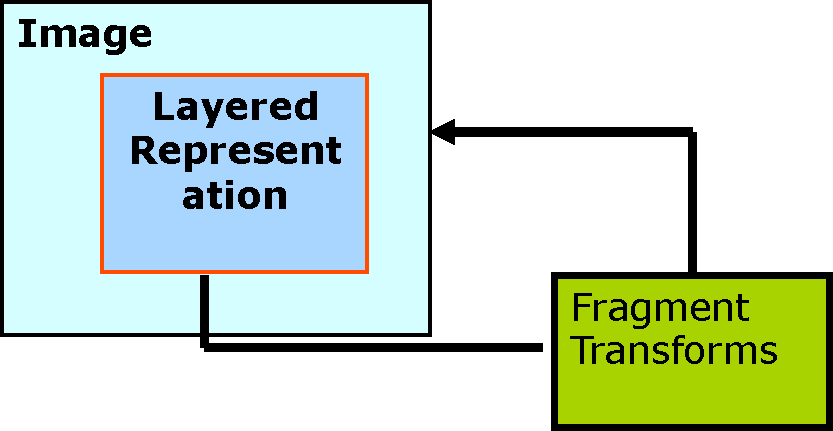
\includegraphics[width=0.4\textwidth]{figs/ma_transforms.pdf}
%% \caption{A high level abstraction of our approach. In this view, our representation serves as a state, and transforms affect this state. This feedback loop hopefully leads to a more organized representation leading to the formation of object parts and proposals. } 
%% \label{fig:ma_transforms}
%% \end{figure}


The multi-layer representation power of our unified representation allows operations on both contours (1 and 2) and regions (3 and 4). Each one of these operations, takes a representation of an image and \emph{transforms} it to another representation of the image by operating in a manner that operations on contours, regions, and appearances are consistent and coupled so that the resulting representation remains the representation of an image:

\begin{definition}
A RECOIN \emph{Transform} is an operation that transforms a RECOIN representation to another RECOIN representation, namely, one that arises from an image.
\label{def:transform}
\end{definition}


%% Since the RECOIN is a complete representation of the image, each RECOIN transform in effect manipulates the image through manipulating the aspects that have been made explicit, \ie, contours, regions, and appearances. Observe that generally a sequence of transforms is needed to delineate an object or an object part. Before discussing the idea of sequences of transforms we outline three essential aspects of an individual transform:

Each transform must deal with defining and implementing three aspects: \emph{(i)} {\bf Detection:} when is a particular transform applicable to a RECOIN representation. For example, if there are no contour gaps because all contours are closed then a gap completion transform is not applicable. On the other hand, if there are multiple gaps, a number of gap completion transforms are applicable; \emph{(ii)} {\bf Transformation:}  This specifies which portions of the representation are removed or modified and what needs to be added to the representation, as concerns contours, regions, and appearances; \emph{(iii)} {\bf Likelihood:} Each transform is a manipulation of proximal data in favor of certain expected regularities. Thus, the extent such a ``hallucination'' takes the representation away from the image data and the extent that it fulfills an expected regularity  (\eg, good continuation) both play a role in determining how likely such a transform moves us toward making sense of the image. Each transform, therefore, requires a measure of likelihood. With these three required aspects, we now formulate each of the four types of transforms in turn. 

%% Each of these four high level actions can be mapped to an individual transformation of our representation. Our process of organizing the image and subsequently forming object proposals is then based on applying a sequence of these individual transformations. Perceptual organization of the image by way of transform sequences requires understanding \emph{when} an individual transform is applicable? and secondly \emph{how} it affects the representation? 

%% As we manipulate the underlying image by continuously applying one transform after another to our representation the first question that arises is which transforms are applicable next? For example, if we take a hypothetical case, where our transformed representation is only composed of a set of closed contours, then the ``Contour Gap Completion'' transform cannot be applied as no gaps exist. This requires that each individual transformation has to define a specific way to {\bf detect} its existence given any individual representation. Assuming we can detect an individual transformation the second question that must be answered is how does its {\bf application} affect the representation? Given that our integrated representation is composed of a shock graph, a set of contours, and a set of regions , what is the exact process for changing these elements? Do all these elements have to change and if so by how much? The answers to these questions depend on the specific transformation under consideration. Finally, while we hope the application of a sequence of transforms leads to meaningful groupings of the image, it is expected that some sequences will lead to erroneous groupings. To minimize the exploration of these non-veridical sequences we assign a {\bf likelihood} to each individual transform. If we look at each step in a sequence as a partial re-organization of the image, this likelihood characterizes the quality of this organization as measured by bottom up image cues (appearance, texture, \etc). The three issues of \emph{(i)} detection: when can a transform be applied, \emph{(ii)} transform process definition: what exact process needs to be applied to the representation, and \emph{(iii)} likelihood/cost: the degree by which the transform makes sense, are therefore central to all four operations. We now address each operation in turn for each of the four types of transformations.

%% , but before we proceed we need to define the local context facing each transform.


%% In what follows we describe these four individual transforms. While each of these tra 

%% each of these individual transforms are performed on 


%% While the affect of a single contour or region based transformation can be quite powerful, in general these partial re-organizations by themselves do not lead to meaningful groupings. More over, the application of a single individual transformation can lead to an erroneous grouping.  Therefore, our process of organizing the image and subsequently forming object proposals is not based on any individual type but rather on the intelligent application of multiple transformations and their combinations to the underlying representation. 


%% In what follows we d


%% each of these four actions as individual transformations and then in the next section discuss how 

%% Before we can discuss the process of applying a transform sequence to our representation, we outline the technical aspects common to all operations that are relevant 


%% affect each individual transform has on our representation. The previous definition of a transformation is rather generic. 


%%  and then in the next Section discuss the idea of sequences of fragment transforms to explore the space of all possible perceptual grouping operations. The first question in finding the sequence of all fragment transforms is to find out which transforms are applicable at any given instance of the representation. This stage is the detection of applicable transforms. The second issue is how perceptually meaningful concepts, such as gap completions, can be effected by transforming the underlying representation. A key point to observe is that since all four types operations are local to the context of the regions/contours under consideration, the transformation likewise needs to remain local in the representation domain. The third issue that is critical when considering a vast set of sequences of transforms is how likely each sequence is, which in turn requires an examination of how likely each individual transform is: the completion of a larger gap requires a greater leap of faith than the completion of a small one. 

%% \begin{definition}
%% The \emph{Local Context} of a Transform is the subset of contours, regions, and shock links/nodes of the RECOIN representation that is affected by the transform. This affect can either be insertion/deletion of any of these elements.
%% \end{definition}

%% \subsection{What is a transformation?}

%% Our reasoning is based on four basic operations: \emph{(1)} introducing new contours, \emph{(2)} removing contours, \emph{(3)} introducing new regions, and \emph{(4)} removing regions. On the surface, these four operations or transformations look very distinct and separate. Contour-based transformations, 1 and 2, seem to suggest we should edit the contour layer , where as region-based transformations, 3 and 4, suggest we should edit the regional layer. How can we express these two seemingly different types of transformation in a common framework? The key is all these transformations, whether regional or contour based, can be mediated by the shock graph. 

%% Transformations of our layered representation amount to editing one of the layers (shock, contours, or regions), mapping those operations through other layers and repeating the process with this new organization. Prior work has looked at the transformations or transitions~\cite{Giblin:Kimia:Reconstruction:PAMI03} of two layers namely the shock graph and its associated closed boundary. Those works showed how a one-parameter family of deformations of the closed boundary change the shock graph layer and vice-versa how editing the shock graph (remove edges,merging nodes) maps to changes of the boundary. Our approach is similar in spirt but we extend those earlier works to look at how changes to a non-closed contour map and its associated shock graph affect each other. Novel to this work, we also show how regional information changes with modifications to the contour map. Given that our goal is to produce object proposals endowed with not only appearance but also shape through way of explicit contours, our operations are defined to transformations initiated by the contour or regional layer only. However, both of these operations can be precisely mediated as changes to the shock graph. 
%% \begin{definition}
%% A transformation reorganizes the image through an operation upon our representation. The operations are defined upon two data-structures or layers of our representation: the shock graph and the set of contours. A transformation of the shock graph is realized through a set of editing operations that delete a subset of shock edges/vertices and insert a new set of shock edges/vertices. A transformation of the contour set is realized through the addition or deletion of a contour. The result of these operations is the formation of a new layered representation. 
%% \label{def:mat}
%% \end{definition}

%% The definition,~\ref{def:mat}, of a transformation is defined in terms of two layers, namely the shock graph and contour layer. It is not necessary to define the transformation in terms of the regional layer or atomic fragments as they are in one to one to correspondence with the shock graph. For example, an equivalent definition would be to say that a transformation of the shock graph is composed of set of editing operations that delete a subset of atomic fragments and insert a new set of atomic fragments. Given this generic definition of a transformation, further questions arise such as how do we \emph{detect} these transformations? What is the cardinality of the set of graph operations and set operations needed to perform a \emph{transformation}? And finally, what is the \emph{likelihood} that this operation leads to a better organization? The answer to these questions depends on the type of transformation under consideration. 

%% \begin{figure*}[ht]
%% \centering
%% \setlength\tabcolsep{0.5pt}
%% \begin{tabular}{cccc}
%% Image & Atomic Fragments & Atomic Fragments with Splicing & Region Growing \\
%% 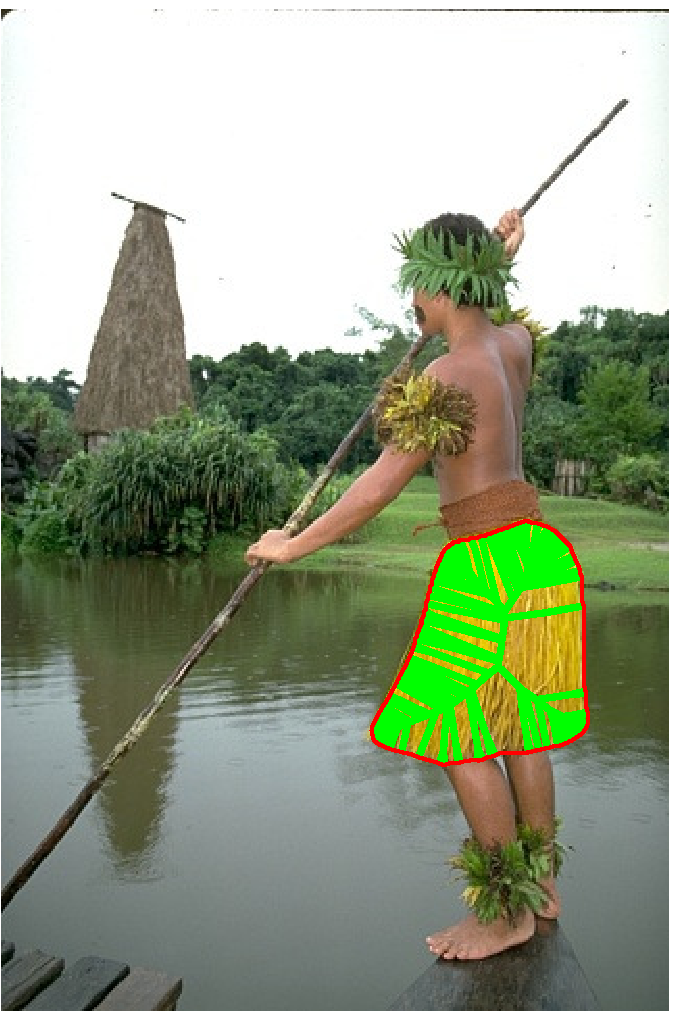
\includegraphics[width=0.25\linewidth]{figs/hulu1.pdf} &
%% 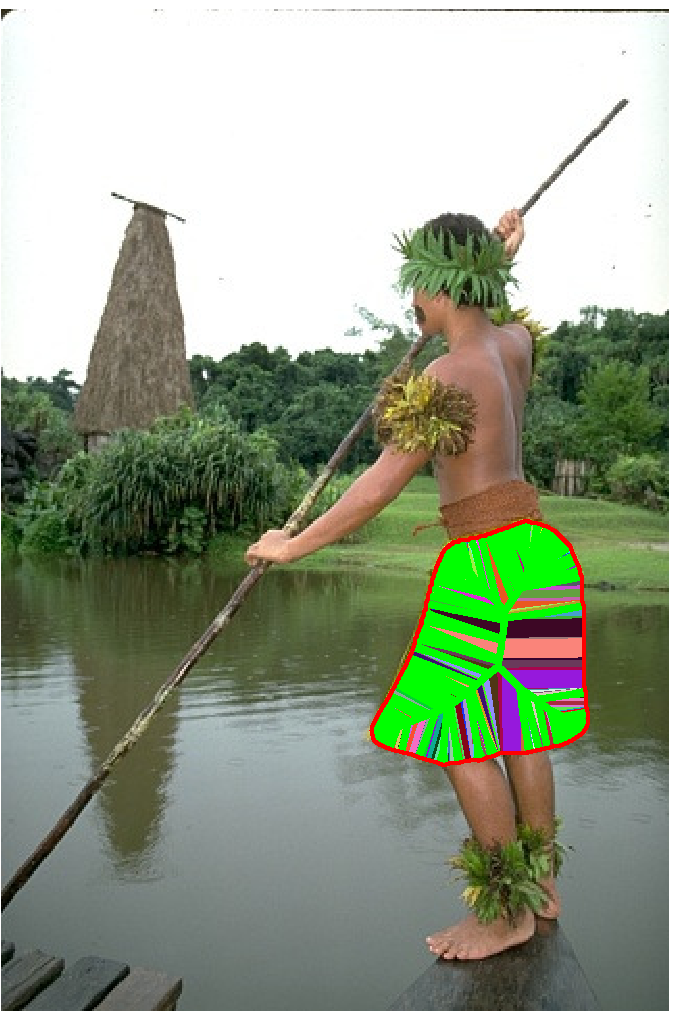
\includegraphics[width=0.25\linewidth]{figs/hulu2.pdf} &
%% 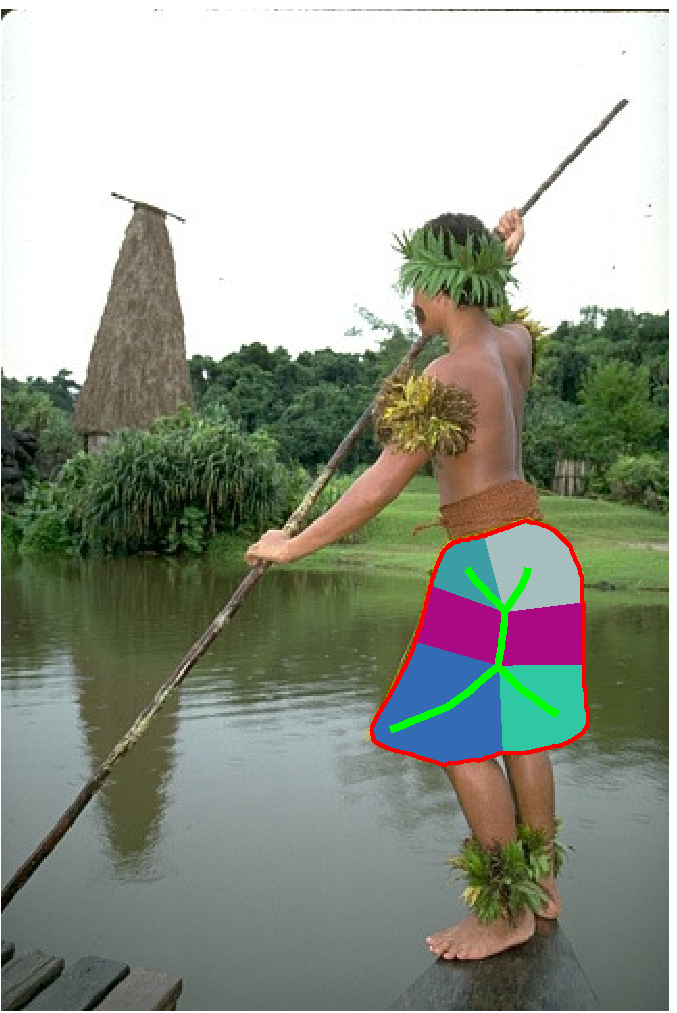
\includegraphics[width=0.25\linewidth]{figs/hulu3.pdf} &
%% 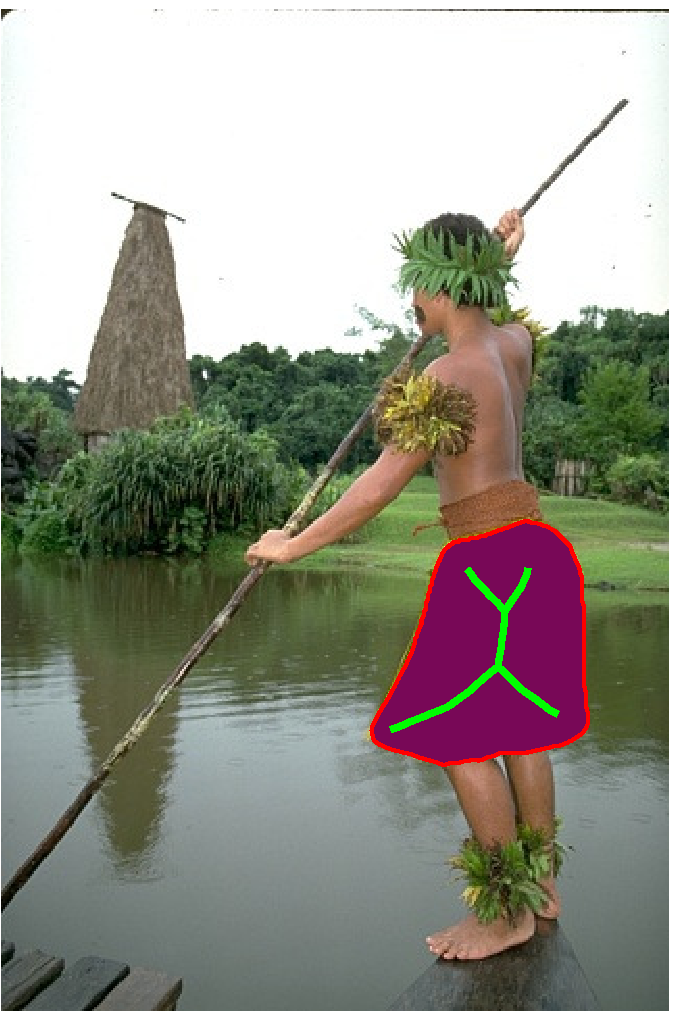
\includegraphics[width=0.25\linewidth]{figs/hulu4.pdf} \\
%% 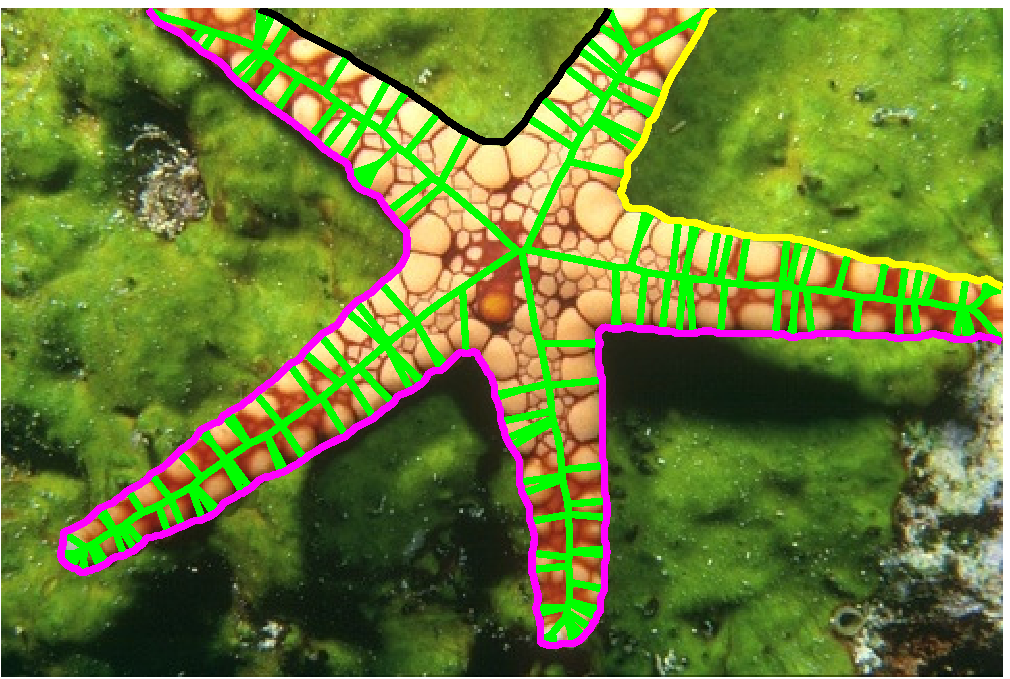
\includegraphics[width=0.25\linewidth]{figs/star1.pdf} &
%% 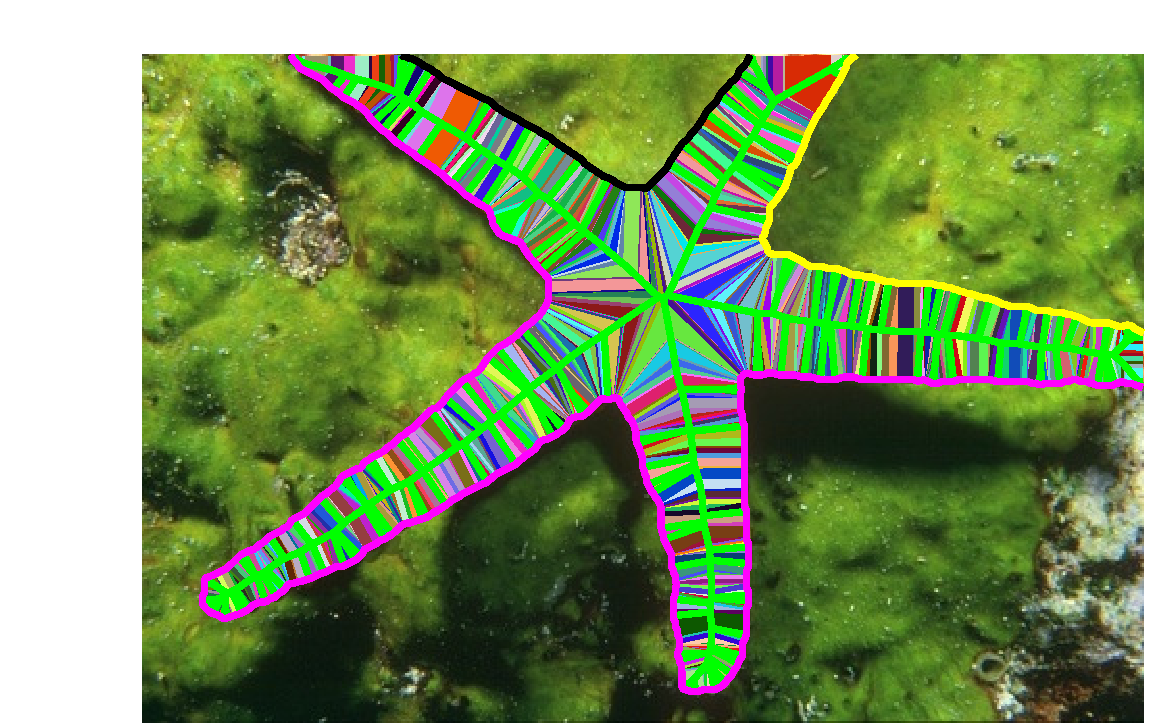
\includegraphics[width=0.25\linewidth]{figs/star3.pdf} &
%% 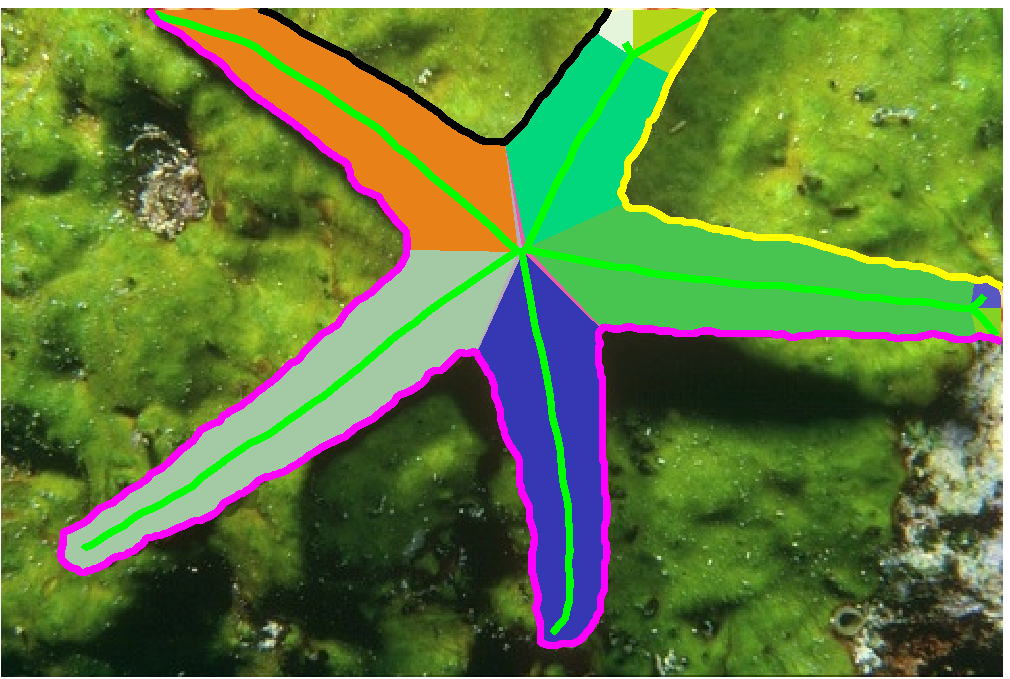
\includegraphics[width=0.25\linewidth]{figs/star4.pdf} &
%% 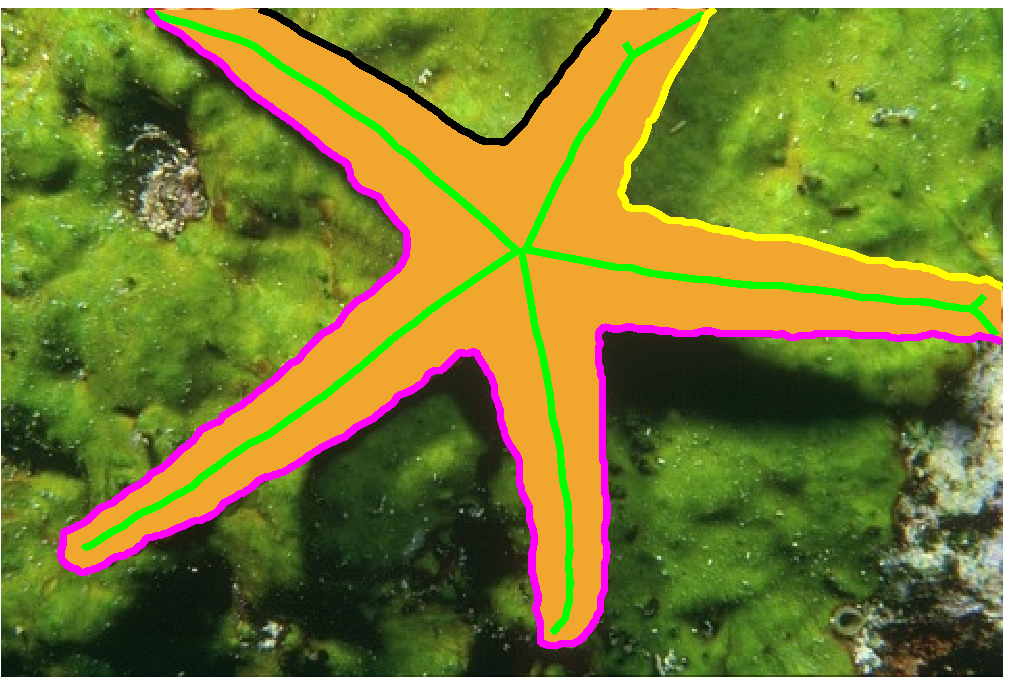
\includegraphics[width=0.25\linewidth]{figs/star5.pdf} \\
%% 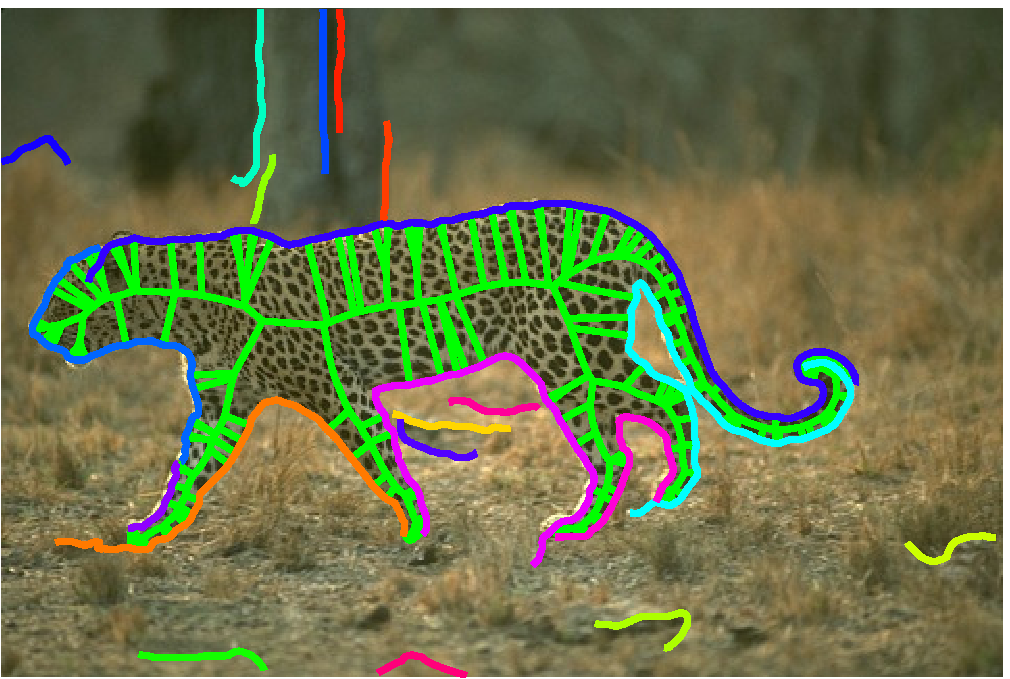
\includegraphics[width=0.25\linewidth]{figs/cheetah1.pdf} &
%% 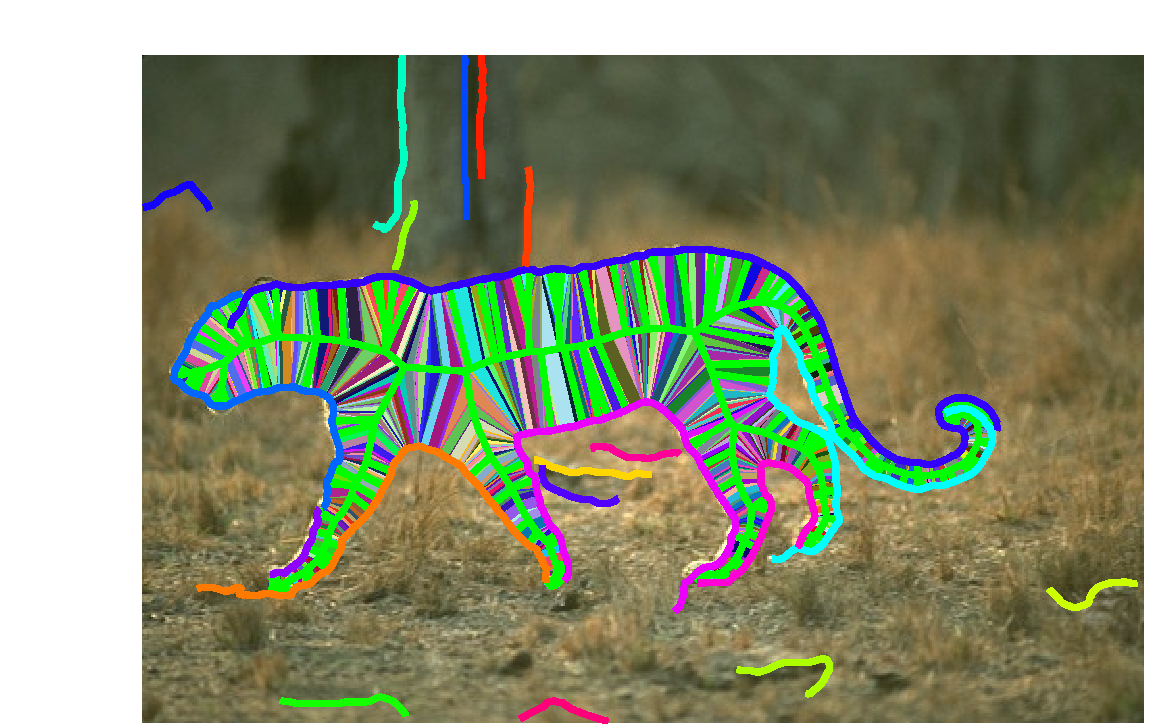
\includegraphics[width=0.25\linewidth]{figs/cheetah2.pdf} &
%% 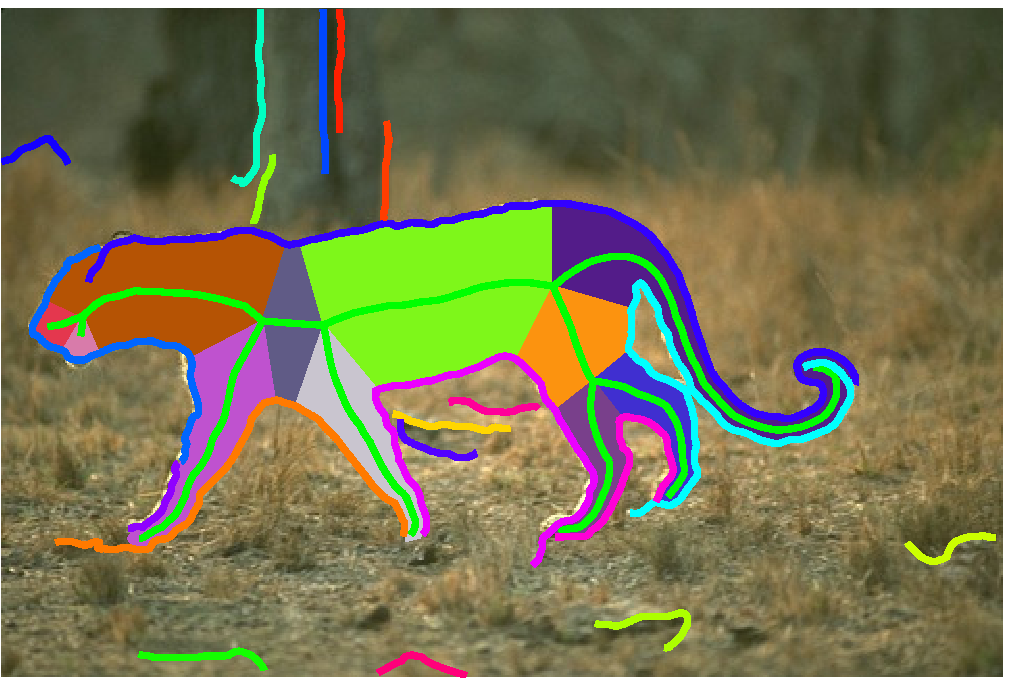
\includegraphics[width=0.25\linewidth]{figs/cheetah3.pdf} &
%% 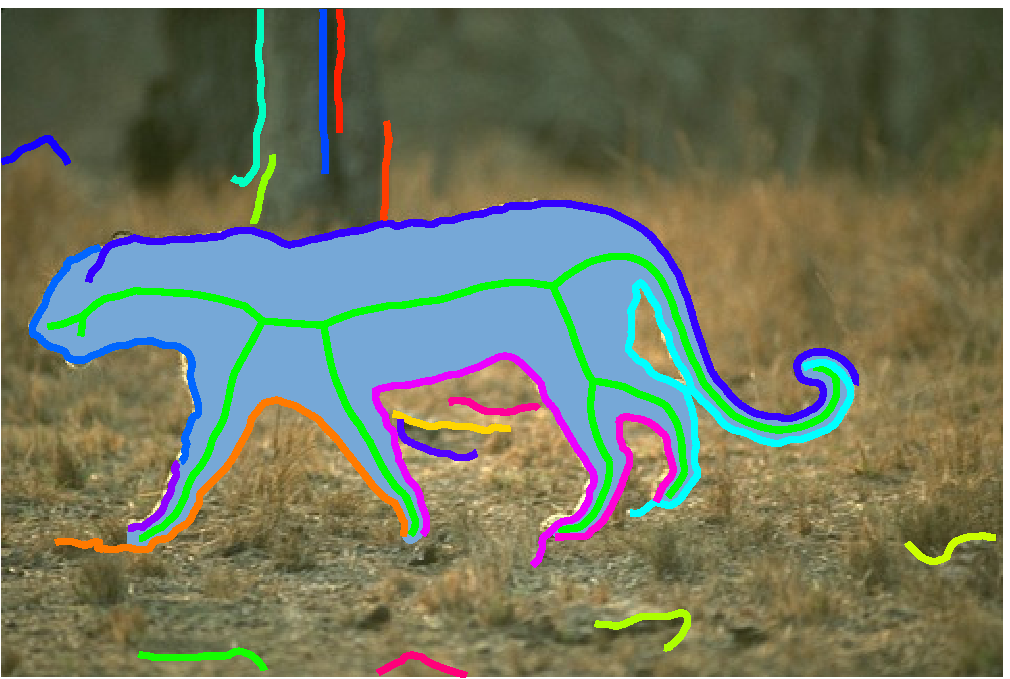
\includegraphics[width=0.25\linewidth]{figs/cheetah4.pdf} \\
%% 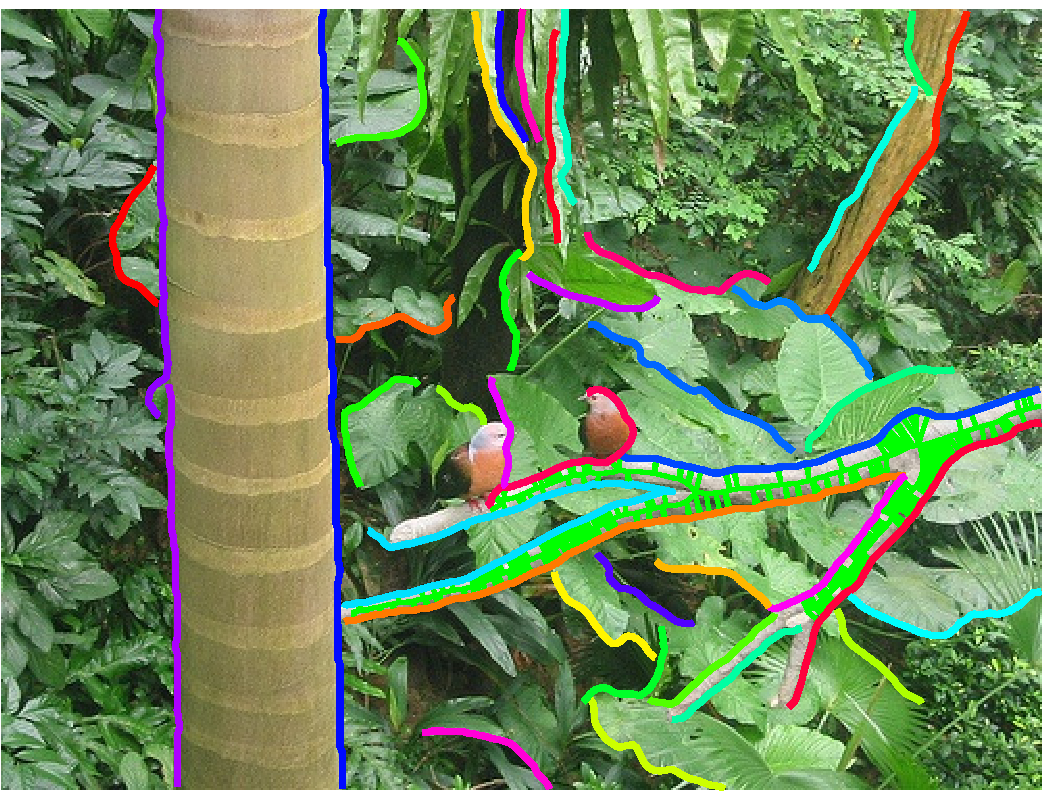
\includegraphics[width=0.25\linewidth]{figs/tree1.pdf} &
%% 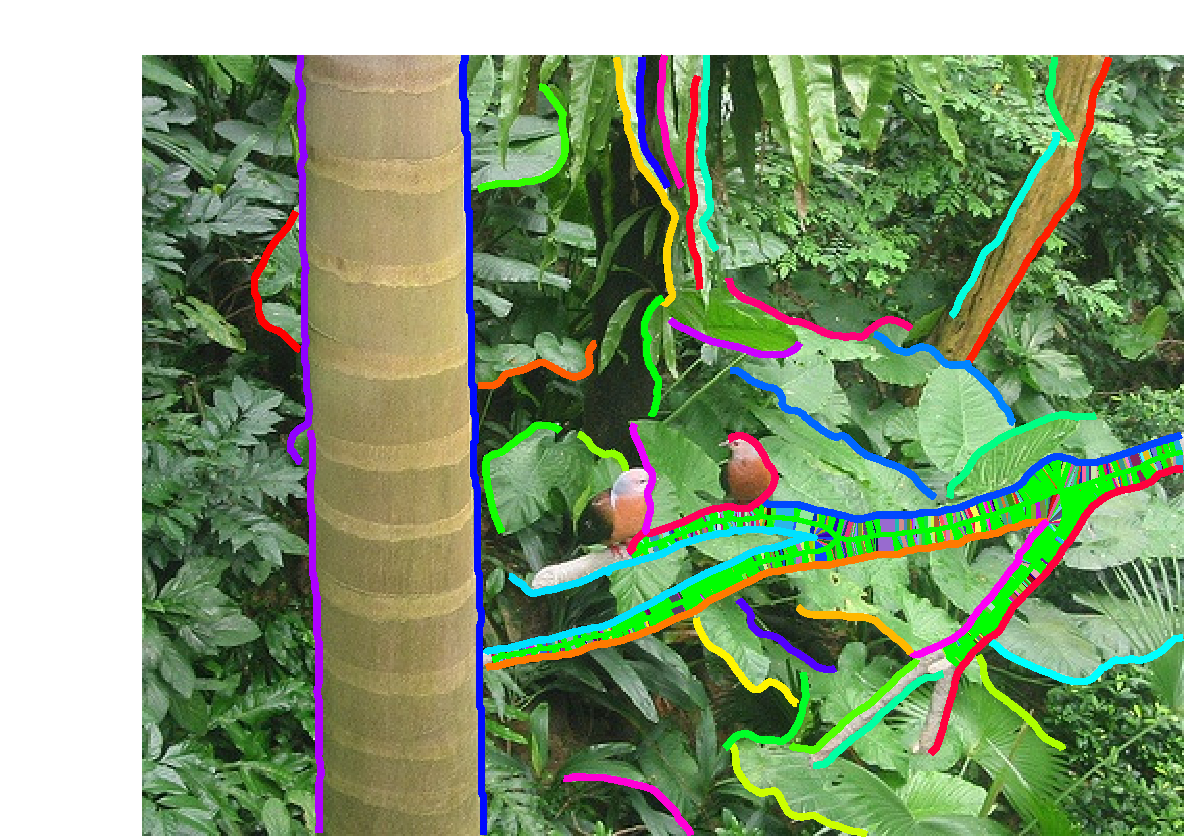
\includegraphics[width=0.25\linewidth]{figs/tree2.pdf} &
%% 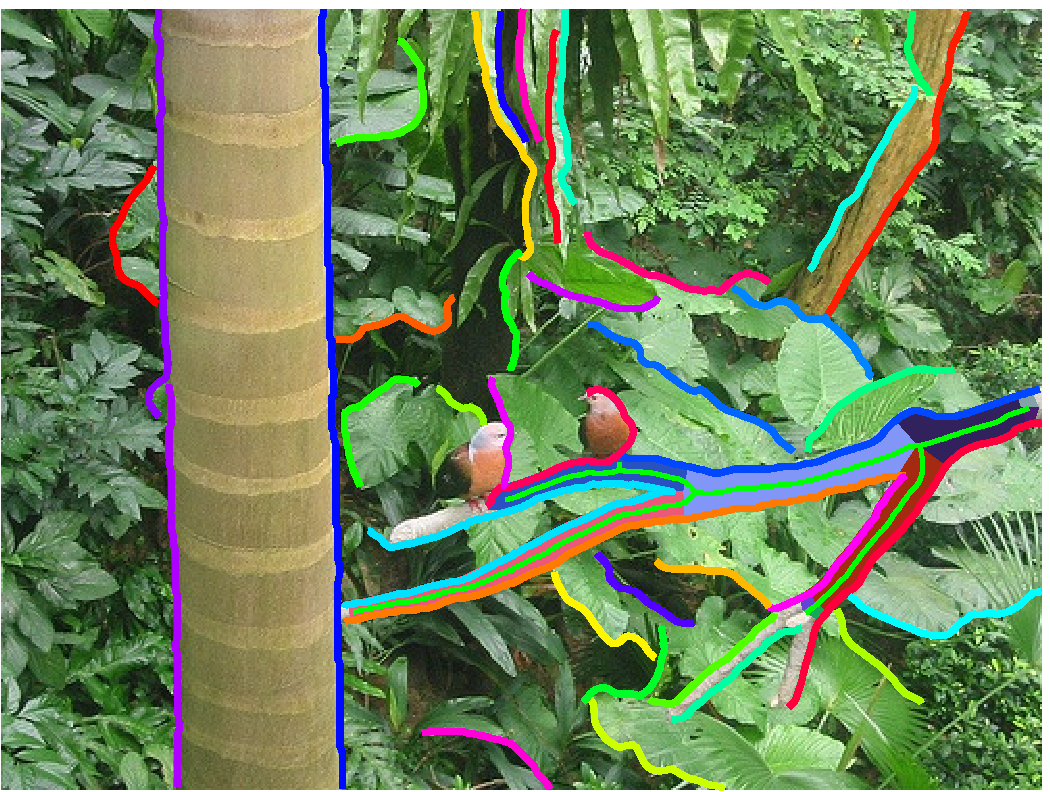
\includegraphics[width=0.25\linewidth]{figs/tree3.pdf} &
%% 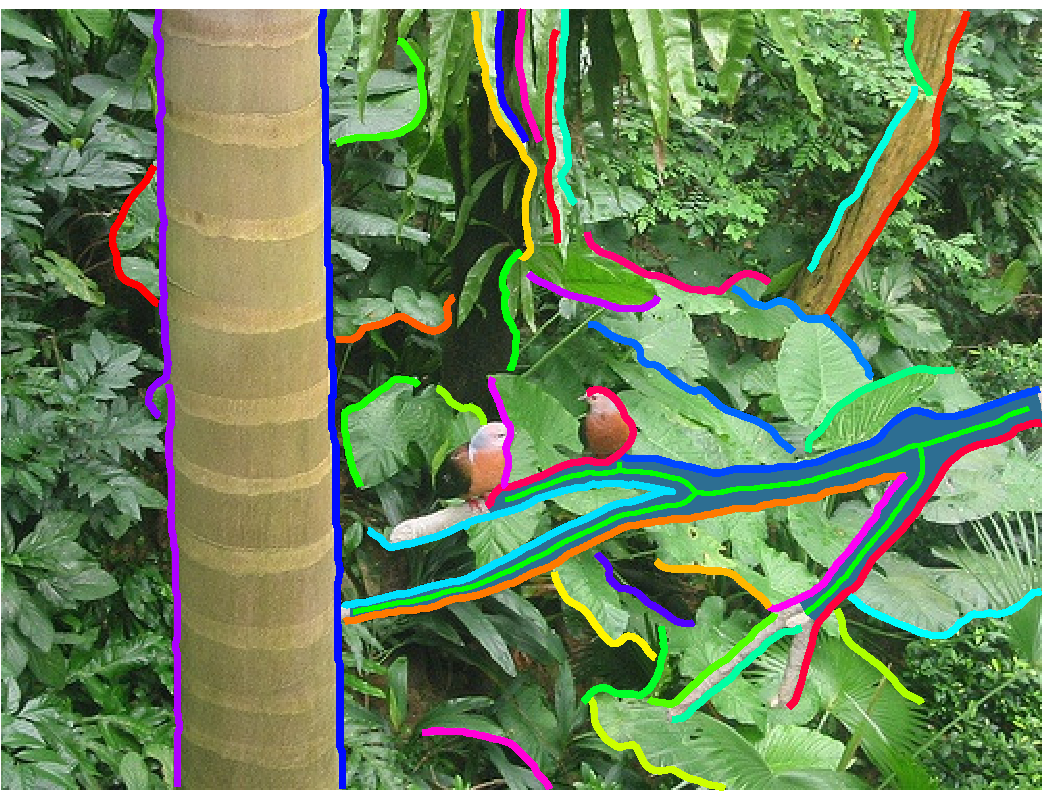
\includegraphics[width=0.25\linewidth]{figs/tree4.pdf} \\
%% \end{tabular}
%% \caption{XXX}
%% \label{fig:splice_example}
%% \end{figure*}


\subsection{Contour-Clutter Removal Transform}

%% \begin{figure*}[!ht]
%% \centering
%% \setlength{\tabcolsep}{2pt}
%% \begin{tabular}{|c|c|c|c|}
%% \hline
%% Local Picture & \textcolor{magenta}{Regions/Shocks} Affected & Remove Elements & Local Shock Computation\\
%% \hline 
%% 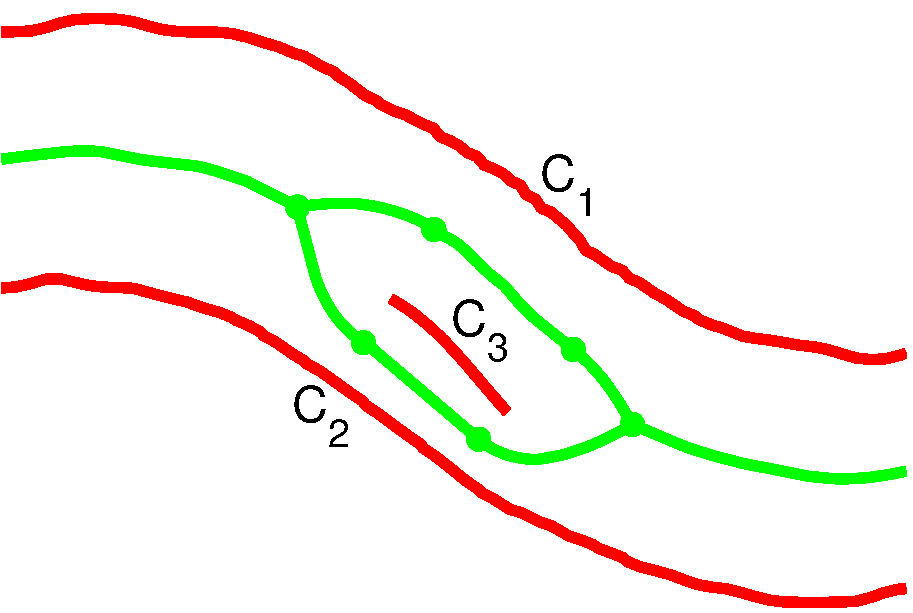
\includegraphics[width=0.24\textwidth]{figs/lsc_l1.pdf} & 
%% 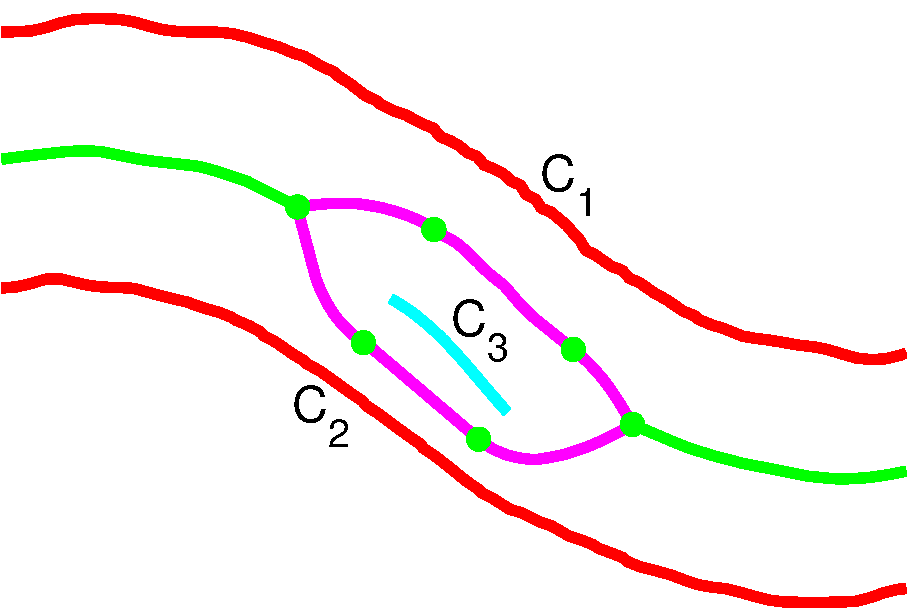
\includegraphics[width=0.24\textwidth]{figs/lsc_l2.pdf} & 
%% 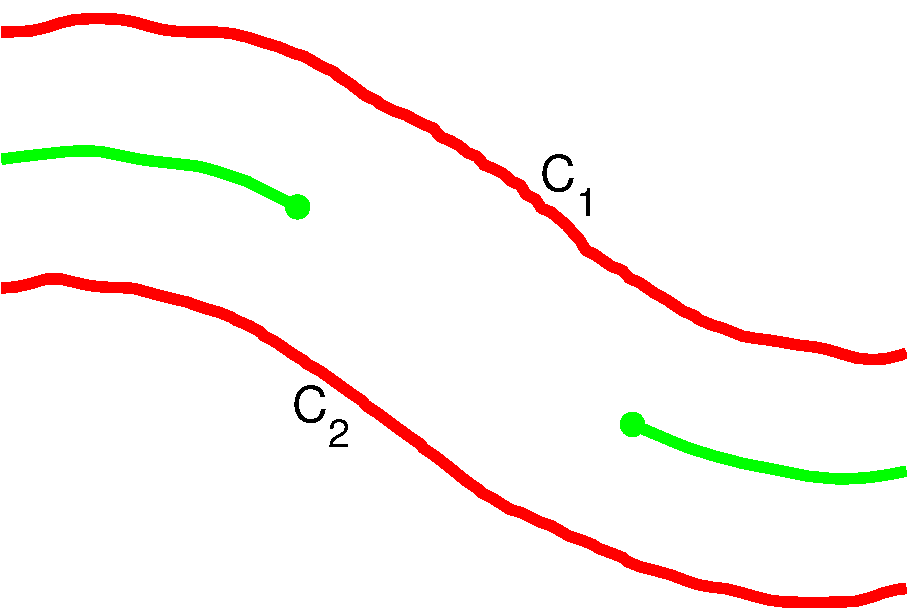
\includegraphics[width=0.24\textwidth]{figs/lsc_l3.pdf} &
%% 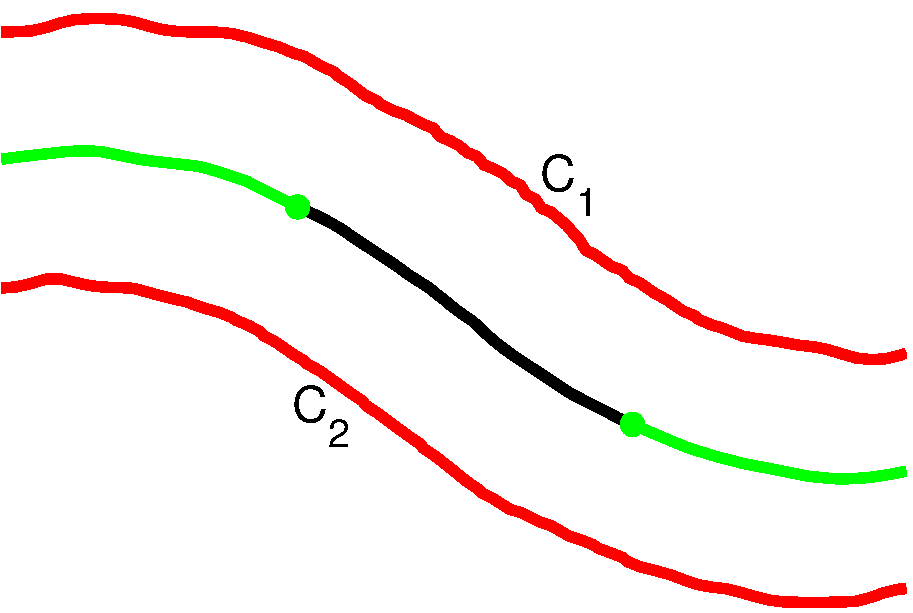
\includegraphics[width=0.24\textwidth]{figs/lsc_l4.pdf} \\
%% 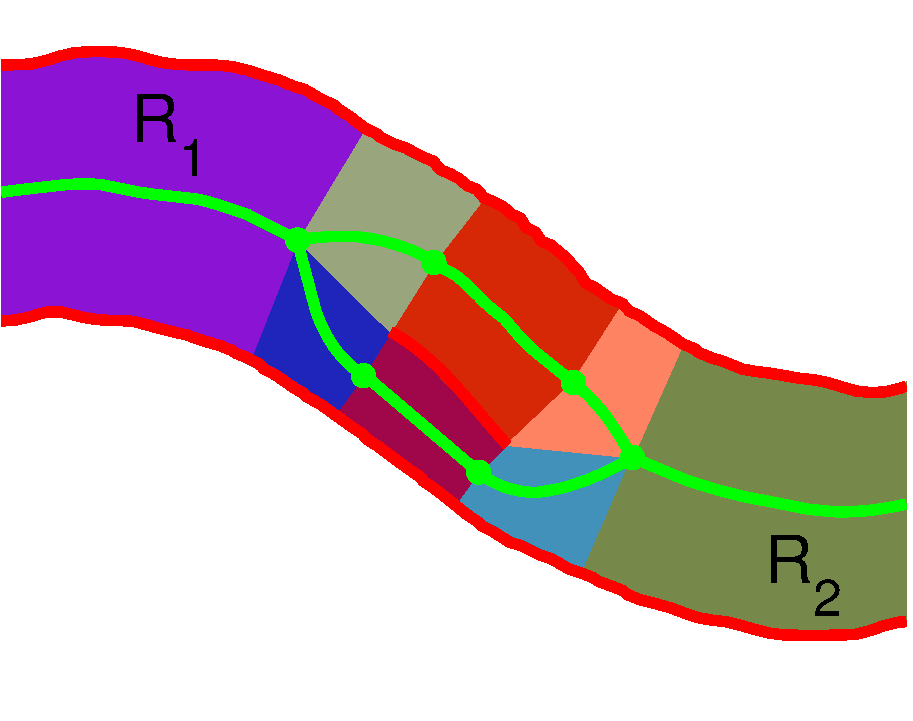
\includegraphics[width=0.24\textwidth]{figs/lsc_l5.pdf}&
%% 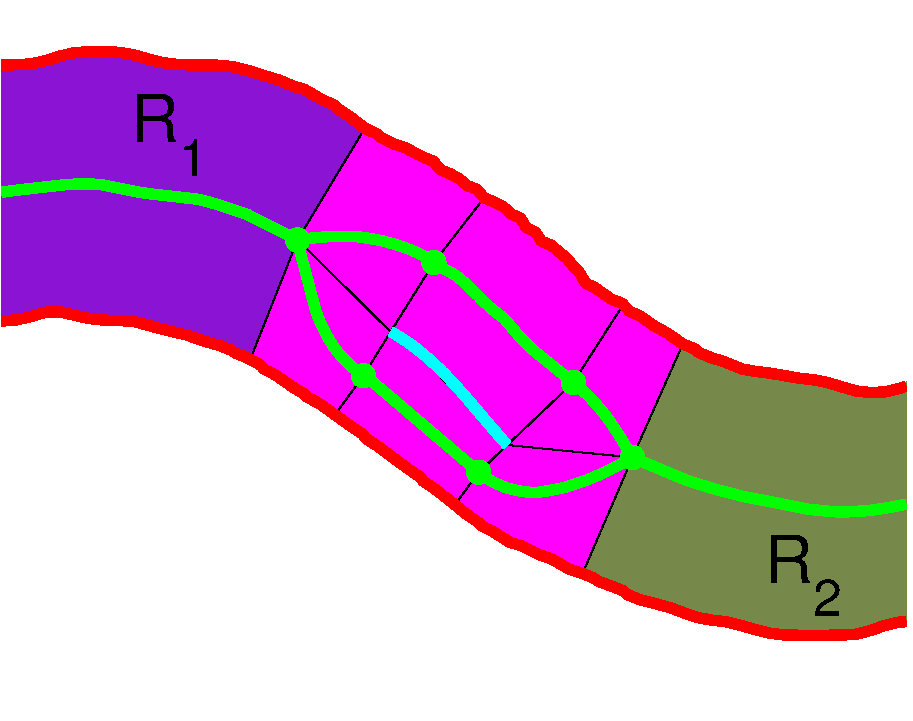
\includegraphics[width=0.24\textwidth]{figs/lsc_l6.pdf}&
%% 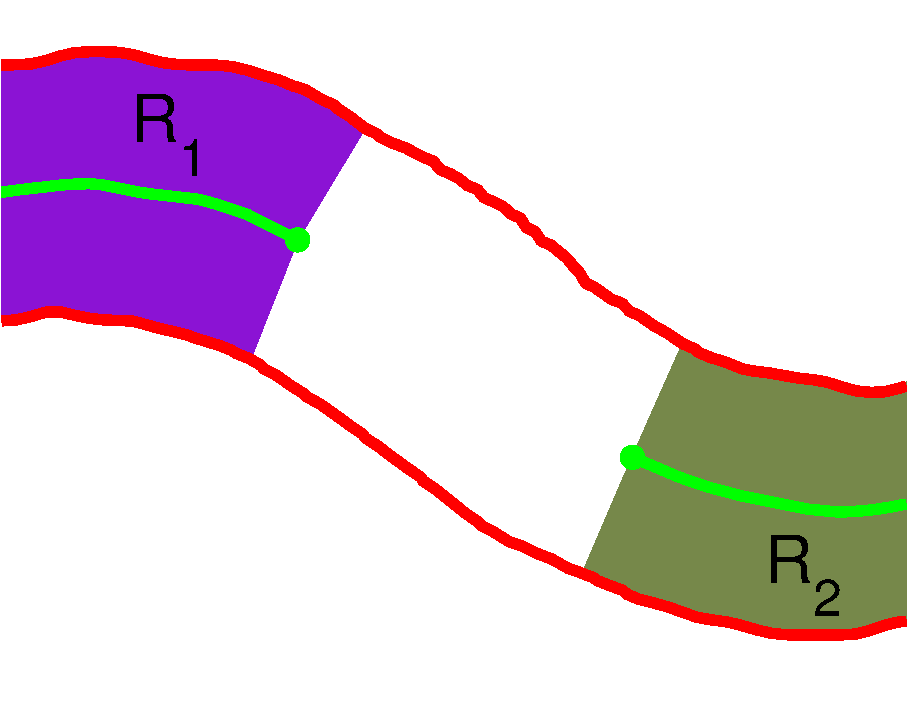
\includegraphics[width=0.24\textwidth]{figs/lsc_l7.pdf}&
%% 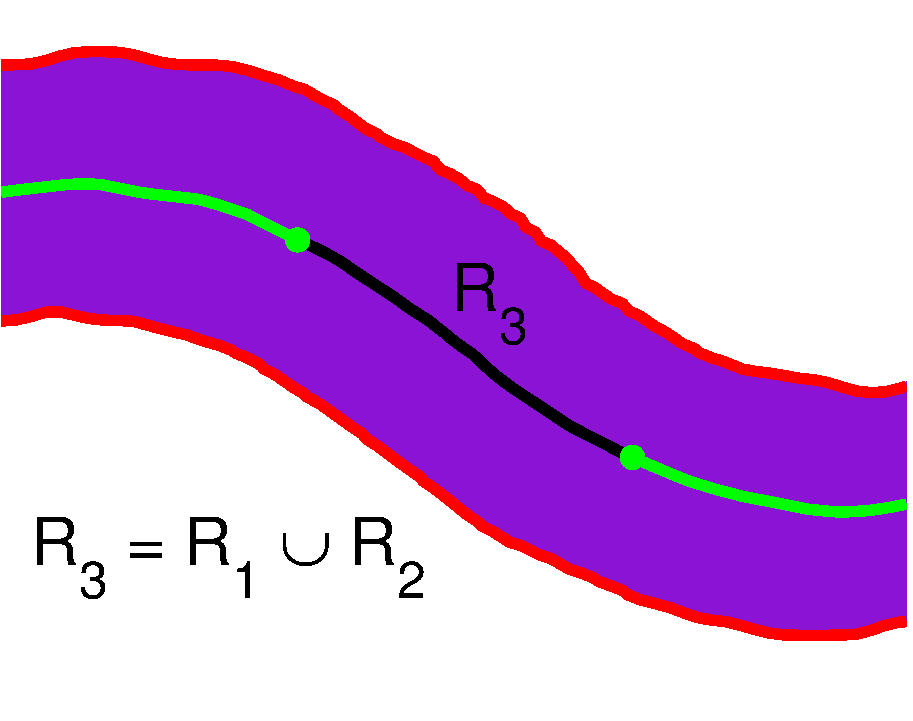
\includegraphics[width=0.24\textwidth]{figs/lsc_l8.pdf}\\
%% \hline
%% \end{tabular}
%% \caption{A local area of our representation where we consider the application of a contour clutter removal transform to contour $C_3$. The removal of $C_3$ highlighted in \textcolor{cyan}{cyan} requires determining the shocks and regions that would be affected. We highlight in \textcolor{magenta}{magenta} the shock links and equivalently the regions that need to be removed. We proceed to remove these elements. Finally, we recompute the new shock links and nodes, highlighted in black, confined to this local area. In the final picture, we can see that the result of this transform has caused regions $R_1$ and $R_2$ to merge into a much larger region.}
%% \label{fig:lc_steps_l1}
%% \end{figure*}

%% \begin{figure*}[!ht]
%% \centering
%%     %% \raisebox{0.10\height}{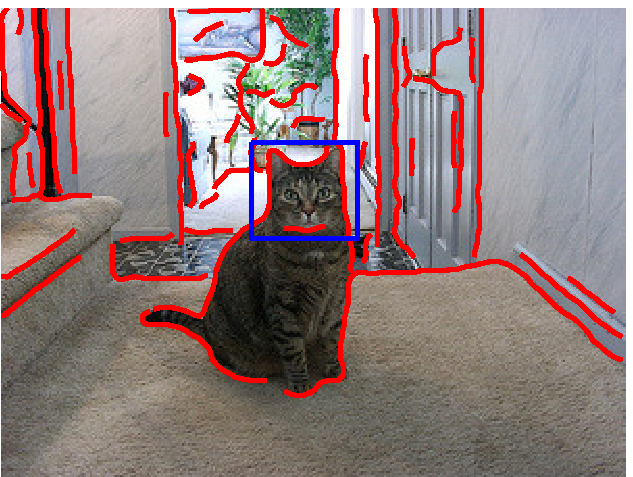
\includegraphics[width=0.20\linewidth]{figs/n02121620_4315_l1.pdf}}&
%%     %% 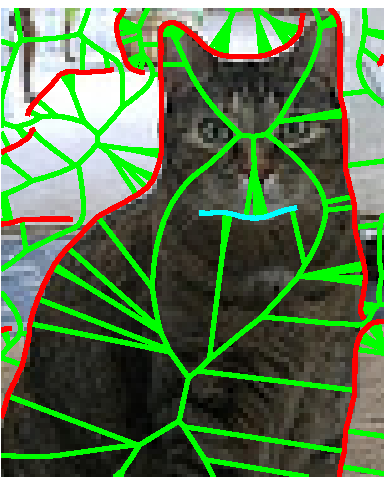
\includegraphics[width=0.15\linewidth]{figs/n02121620_4315_l1_before_shocks.pdf} &
%%     %% 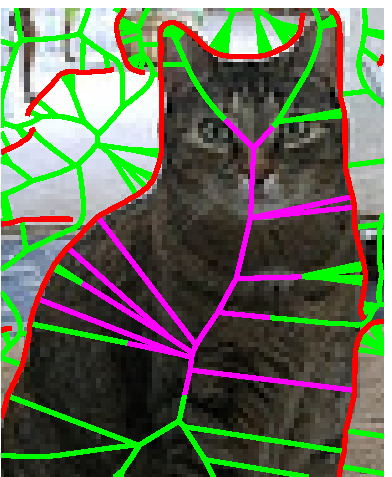
\includegraphics[width=0.15\linewidth]{figs/n02121620_4315_l1_after_shocks.pdf} &
%%     %% 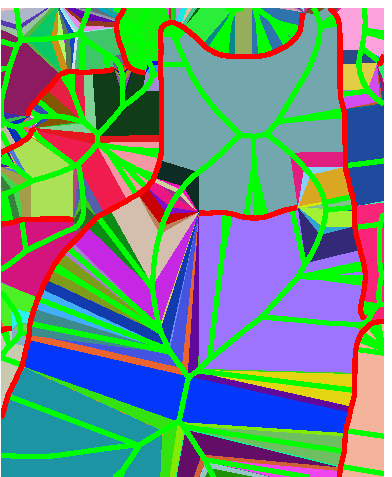
\includegraphics[width=0.15\linewidth]{figs/n02121620_4315_l1_before_frags.pdf} &
%%     %% 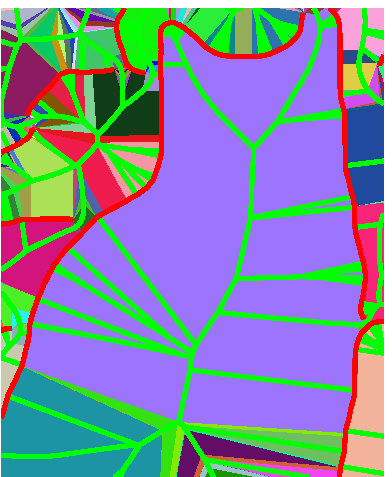
\includegraphics[width=0.15\linewidth]{figs/n02121620_4315_l1_after_frags.pdf} \\
%%     %% \hline
%%     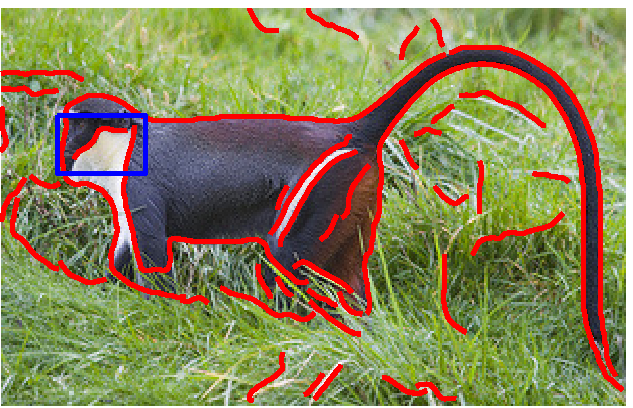
\includegraphics[width=0.10\linewidth]{figs/n02484322_9968_l1.pdf}
%%     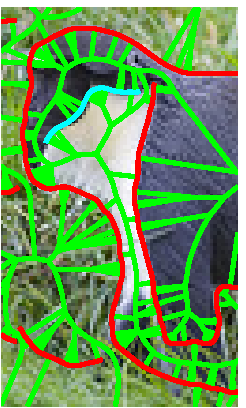
\includegraphics[width=0.10\linewidth]{figs/n02484322_9968_l1_before_shocks.pdf}
%%     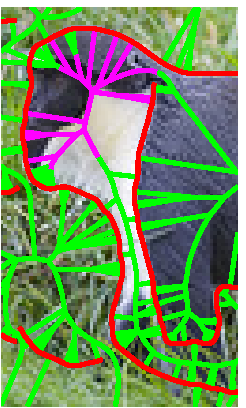
\includegraphics[width=0.10\linewidth]{figs/n02484322_9968_l1_after_shocks.pdf} 
%%     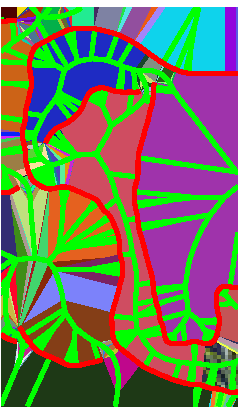
\includegraphics[width=0.10\linewidth]{figs/n02484322_9968_l1_before_frags.pdf} 
%%     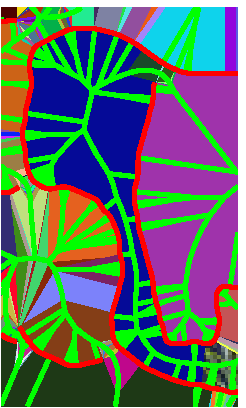
\includegraphics[width=0.10\linewidth]{figs/n02484322_9968_l1_after_frags.pdf} 

%%     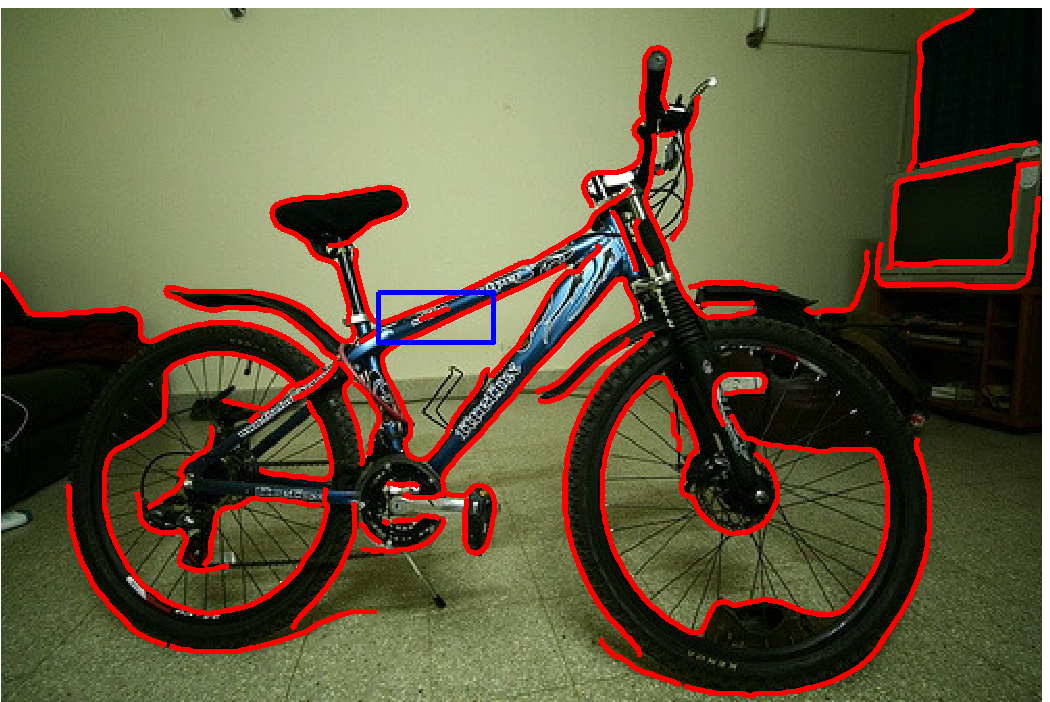
\includegraphics[width=0.18\linewidth]{figs/002227_loop_l1.pdf} 
%%     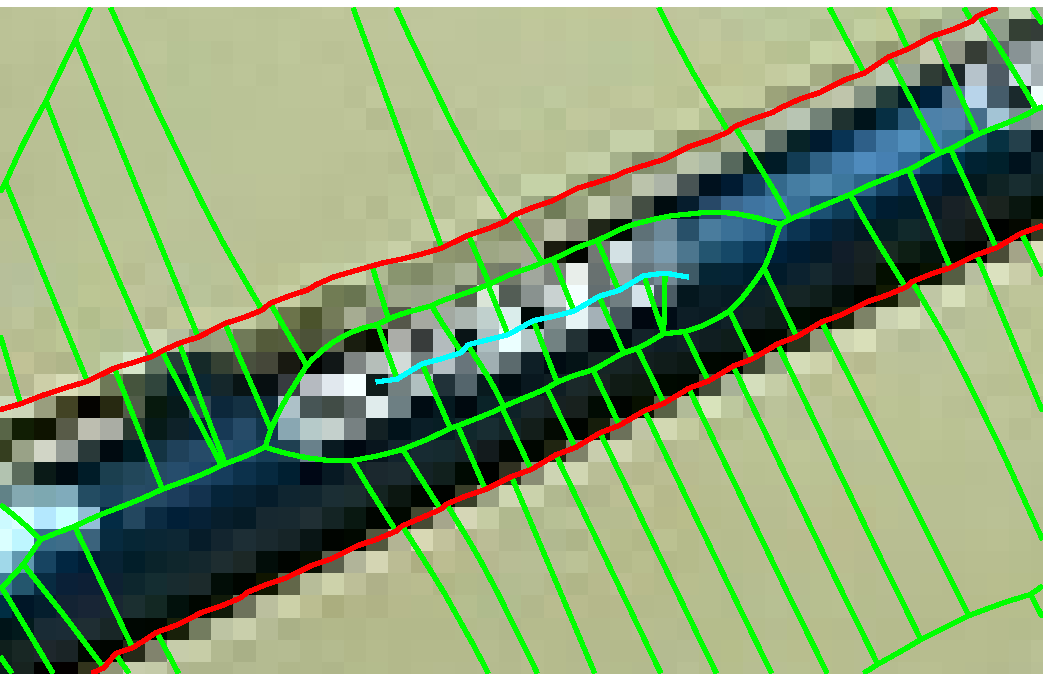
\includegraphics[width=0.18\linewidth]{figs/002227_l1_before_shocks.pdf}
%%     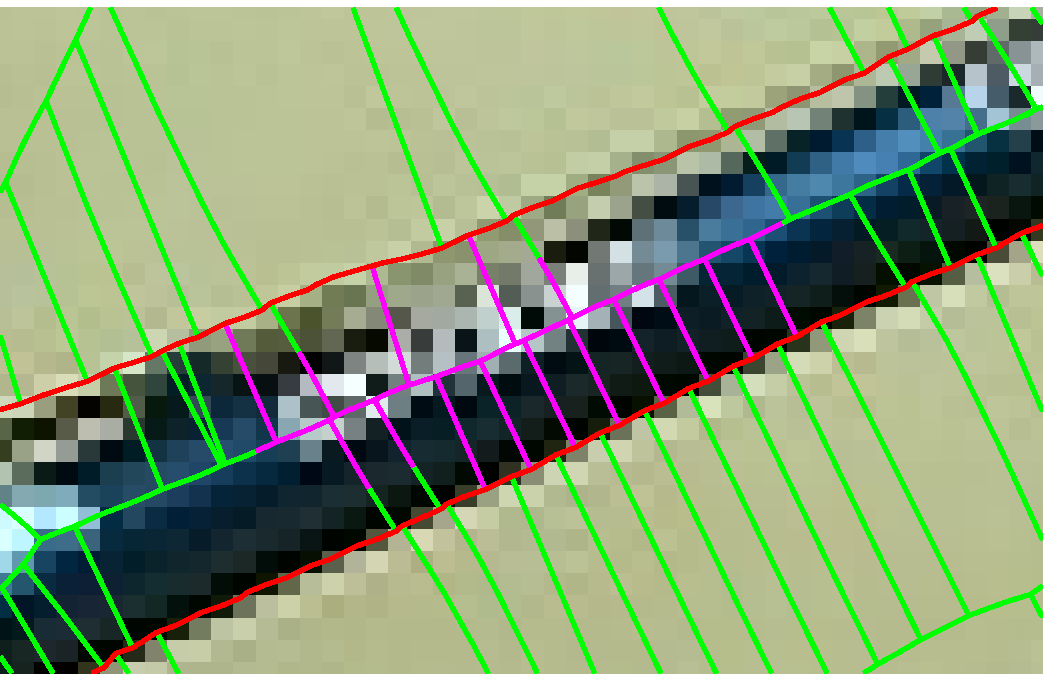
\includegraphics[width=0.18\linewidth]{figs/002227_l1_after_shocks.pdf} 
%%     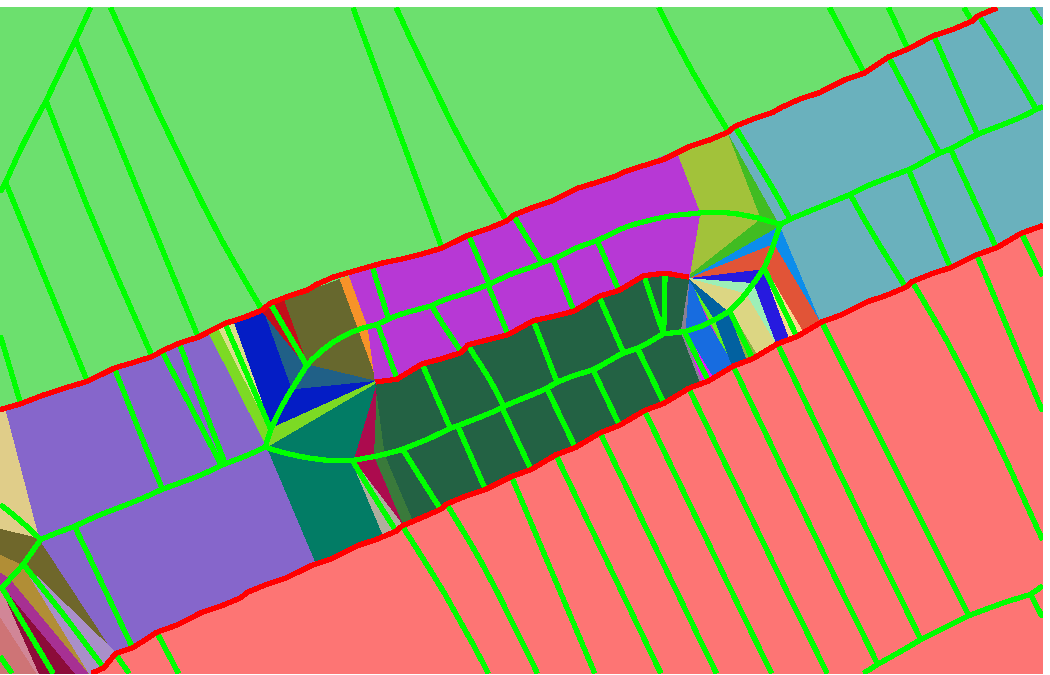
\includegraphics[width=0.18\linewidth]{figs/002227_l1_before_frags.pdf}
%%     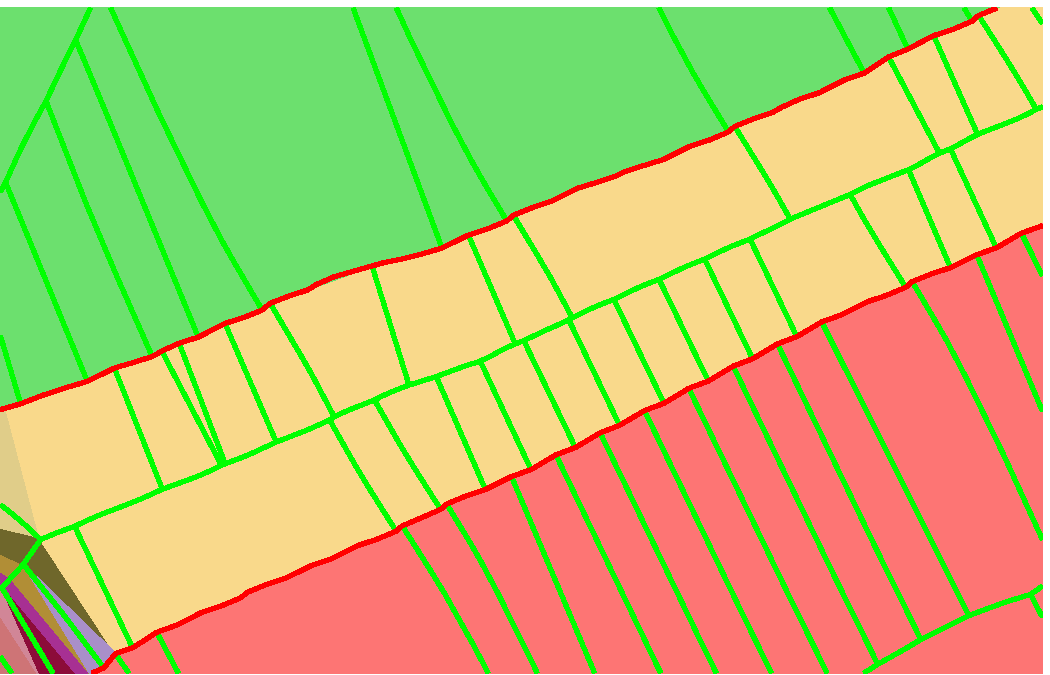
\includegraphics[width=0.18\linewidth]{figs/002227_l1_after_frags.pdf}
%%     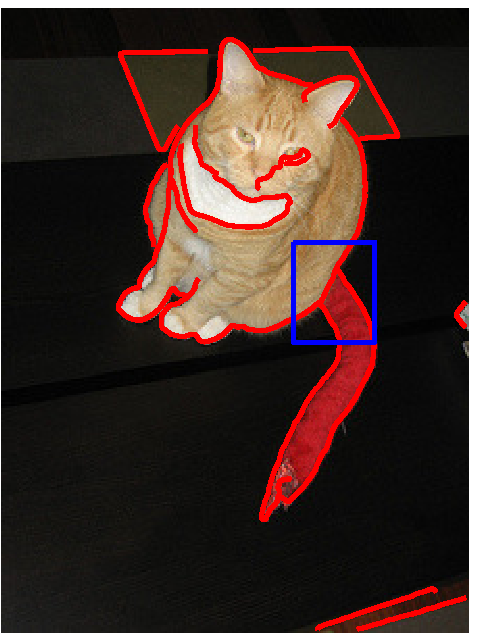
\includegraphics[width=0.20\linewidth]{figs/n02121620_11528_l1.pdf} 
%%     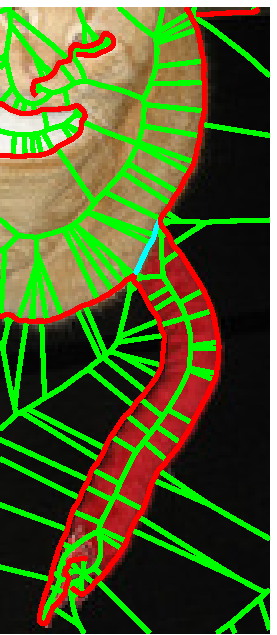
\includegraphics[width=0.23\linewidth]{figs/n02121620_11528_l1_before_shocks.pdf}
%%     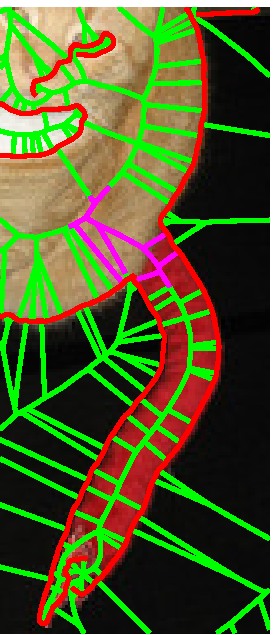
\includegraphics[width=0.23\linewidth]{figs/n02121620_11528_l1_after_shocks.pdf} 
%%     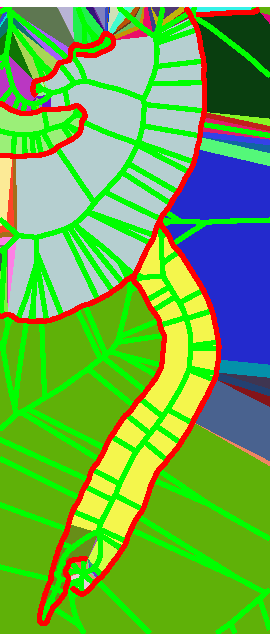
\includegraphics[width=0.23\linewidth]{figs/n02121620_11528_l1_before_frags.pdf} 
%%     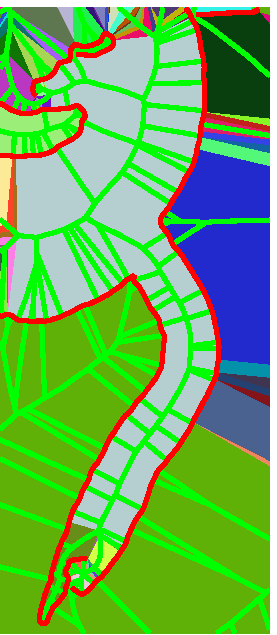
\includegraphics[width=0.23\linewidth]{figs/n02121620_11528_l1_after_frags.pdf}
%%   \caption{Different examples of the clutter-removal transform being applied to local areas of various images. }
%%   \label{fig:real_loop}
%% \end{figure*}


Fragments that correspond to objects have boundaries that are silhouettes. Since image contours include not only silhouettes, but also reflection boundaries, surface definition contours, \etc, a process must discard these distracting contours \ie, ``clutter contours'' so that the resulting fragments can reflect the underlying objects, Figure~\ref{fig:loop_transforms}. In absence of an explicit labeling (silhouette/non-silhouette), those contour segments which are likely non-silhouette should be removed to observe the outcome. 


\begin{figure*}[!ht]

\footnotesize{\textit{a}} 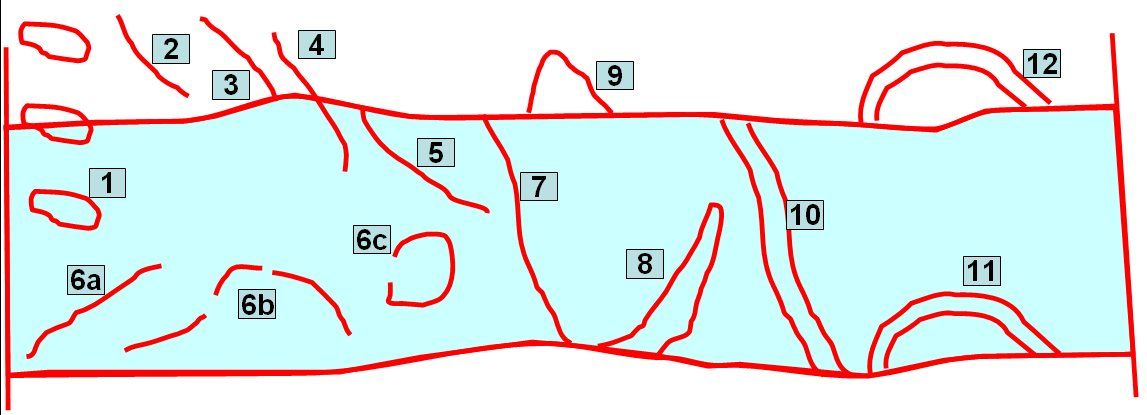
\includegraphics[height=0.06\linewidth]{figs/all-loop-cases.jpg}
\footnotesize{\textit{b}}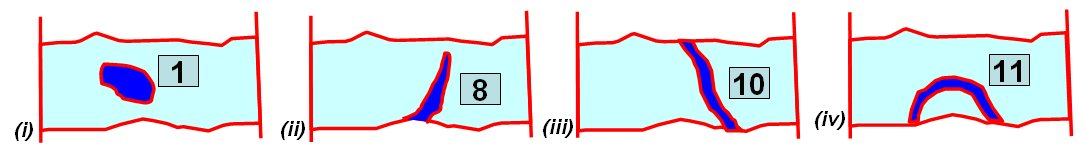
\includegraphics[height=0.06\linewidth]{figs/refined-all-loop-cases-1.jpg}
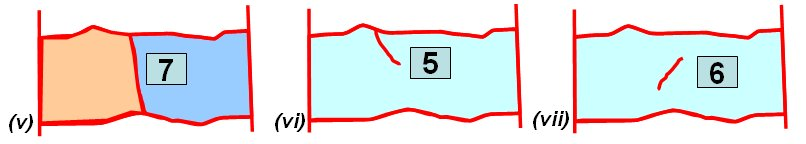
\includegraphics[height=0.06\linewidth]{figs/refined-all-loop-cases-2.jpg}
\centerline{
%\includegraphics[width=0.10\linewidth]{figs/fragment-no-contamination.jpg}
 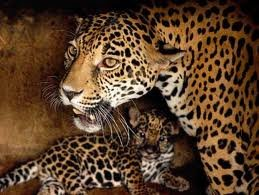
\includegraphics[height=0.110\linewidth]{figs/leopard.jpg}
 \includegraphics[height=0.110\linewidth]{figs/horse61.jpg} 
 \includegraphics[height=0.110\linewidth]{figs/shamu-1.jpg}
 \includegraphics[height=0.110\linewidth]{figs/tiger-1.jpg}  
\includegraphics[height=0.110\linewidth]{figs/zebra-1.jpg}
\includegraphics[height=0.110\linewidth]{figs/horse6.jpg}  
\includegraphics[height=0.110\linewidth]{figs/horse49.jpg}  
}
%\vspace{-0.6cm}
\caption{(a)We use a sketch of a normative object part, the horizontal cyan
strip, to systematically derive all possible ways a spurious contour can
 interfere with its formation, leading to  seven
principal cases, as in(b). These can be easily recognized in natural images (c), \eg, leopard spots, markings off a whale, tiger stripes,
\etc  The removal of these effects is key to the formation of object part hypotheses.}
   \label{fig:loop_transforms}
   %\vspace{-0.75cm}
\end{figure*}


%% The reason why this operation is needed is that not all contour fragments belong to the silhouette of an object of interest, \eg , internal contours. These contours need to be removed before the object can properly be organized/discovered. These internal or spurious contours which often explain the 3D local form, object texture, reflectance, \etc, are only spurious in the sense that they interfere with the formation of an object or object part silhouette.  illustrates the wide variety of potential curves that the algorithm considers for removal.





\noindent\\
{\bf Detection:} The removal of contours interfering with object formation, as shown in Figure~\ref{fig:loop_transforms}, can be classified into two distinct groups: \emph{(i) single contours} such as cases (2, 3, 4, 5, 6, 7) and \emph{ (ii) double contours that enclose a region} such as cases (1, 8, 9, 10, 11, 12). The former case of single contours are the subject of the \emph{contour clutter removal transform}, while the latter cases are the subject of the \emph{region clutter removal transform}, Section~\ref{sec:region_clutter}. Single contours can be open or closed or possibly intersecting another boundary forming a junction (T, X, Y, \etc). Single contours prevent the formation of a fragment between silhouette curves by interfering with waves propagating from the boundaries causing extraneous shock branches to form, Figure~\ref{fig:loops}. Instead the single contour interacts with silhouettes ( or other clutter contours) to form a \emph{loop} in the shock graph. Thus, if the shock graph is the sole underlying representation, as was the case in~\cite{Johannes:POCV2001}, the transform requires a detection of simple cycles in the shock graph. However, our RECOIN representation has simultaneous access to contours, regions, and shocks. It is far simpler then to consider removing a single contour than it is to search for cycles in the shock graph, thus making detection of when this transform is applicable trivial.


\begin{figure}[!ht]
\centering
\includegraphics[width=0.31\textwidth]{figs/loop-waves.pdf}
\caption{ Waves $W_1$ and $W_2$ are quenched by waves from the spurious boundary, $W_s$, resulting in a loop in the shock structure. } 
\label{fig:loops}
\end{figure}

%% to form in the shock graph. Therefore, transformations of this type can be detected by looking for cycles in the shock graph, and this is what was done in an earlier phase of research when only the shock graph was present. However, our RECOIN representation has simultaneous access to contours, regions, and shocks, and therefore it is much simpler and straightforward to simply look at contours themselves as candidates for removal. Thus, the detection step becomes very simple: each contour fragment is a candidate to be considered as a clutter contour. 



%% \begin{figure*}[!ht]
%% \centering
%% \setlength{\tabcolsep}{2pt}
%% \begin{tabular}{cc}
%% {\footnotesize\textit{\textcolor{black}{a)}}}\includegraphics[width=0.11\textwidth]{figs/bear_l1.pdf}&\multirow{3}{*}[0.45in]{{\footnotesize\textit{\textcolor{black}{d)}}}\includegraphics[width=0.3\textwidth]{figs/bear_l4.pdf}}\\
%% {\footnotesize\textit{\textcolor{black}{b)}}}\includegraphics[width=0.11\textwidth]{figs/bear_l2.pdf}\\
%% {\footnotesize\textit{\textcolor{black}{c)}}}\includegraphics[width=0.11\textwidth]{figs/bear_l3.pdf}\\
%% \end{tabular}
%% \begin{tabular}{cc}
%% {\footnotesize\textit{\textcolor{black}{e)}}}\includegraphics[height=0.09\textwidth]{figs/cat1.pdf}&\multirow{3}{*}[0.45in]{{\footnotesize\textit{\textcolor{black}{h)}}}\includegraphics[width=0.3\textwidth]{figs/cat4.pdf}}\\
%% {\footnotesize\textit{\textcolor{black}{f)}}}\includegraphics[height=0.09\textwidth]{figs/cat2.pdf}\\
%% {\footnotesize\textit{\textcolor{black}{g)}}}\includegraphics[height=0.09\textwidth]{figs/cat3.pdf}\\
%% \end{tabular}
%% \caption{a,e) We show two examples where we are considering the removal of the \textcolor{cyan}{cyan} curve surrounded by the \textcolor{red}{red} silhouette curve. For clarity we have removed the shock graph. b,f) If we look at the initial set of fragmented medial visual fragments we see that the effect of removing this contour causes all regions to merge in both cases. d,h) The merging of $N$ regions to 1 can be expressed as a region hierarchy.}
%% \label{fig:loop_cost}
%% \end{figure*}



%% \begin{figure*}[!ht]
%% \centering
%% \setlength{\tabcolsep}{2pt}
%% \begin{tabular}{|ccc|ccc|}
%% \hline
%% \raisebox{0.1\height}{\includegraphics[width=0.17\textwidth]{figs/bear_l1.pdf}}&
%% \raisebox{0.1\height}{\includegraphics[width=0.17\textwidth]{figs/bear_l2.pdf}}&
%% \raisebox{0.1\height}{\includegraphics[width=0.17\textwidth]{figs/bear_l3.pdf}}&
%% \includegraphics[width=0.15\textwidth]{figs/cat1.pdf}&
%% \includegraphics[width=0.15\textwidth]{figs/cat2.pdf}&
%% \includegraphics[width=0.15\textwidth]{figs/cat3.pdf}\\
%% \multicolumn{3}{|c|}{\includegraphics[width=0.45\textwidth]{figs/bear_l4.pdf}}&
%% \multicolumn{3}{|c|}{\includegraphics[width=0.45\textwidth]{figs/cat4.pdf}}\\
%% \hline
%% \end{tabular}
%% \caption{We show two examples where we are considering the removal of the \textcolor{cyan}{cyan} curve surrounded by the \textcolor{red}{red} silhouette curve. For clarity we have removed the shock graph. If we look at the initial set of fragmented medial visual fragments we see that the effect of removing this contour causes all regions to merge in both cases. The merging of $N$ regions to 1 can be expressed as a region hierarchy.}
%% \label{fig:loop_cost}
%% \end{figure*}





\noindent\\
{\bf Transformation:} It might appear that the transformation process of contour clutter removal is trivial: simply remove the contour fragment from the set of all contour fragments. However, the advantage of having multiple explicit representations comes with a price: the redundancy requires synchronization of the transformation process along all the coupled layers, namely, changes to the contour map require simultaneous and constant changes to the shock graph and to the regional representation. Figure~\ref{fig:lc_steps_l1} highlights the steps in this process from left to right. In this example, the interaction of silhouette contours $C_1$ and $C_2$ is ``interrupted'' by the ``clutter contour'' $C_3$, creating a loop in the shock graph as shown in Figure~\ref{fig:lc_steps_l1}\textcolor{red}{a}. Similarly, the regional representation is fragmented into many disjoint regions due to $C_3$ restricting the formation of a singular region between $C_1$ and $C_2$. 



%% In terms of the regional representation, the presence of the clutter contour, $C_3$, between $C_1$ and $C_2$ has resulted in a set of fragmented regions. 


%% We seek all shock links/nodes that arise from $C_3$ since they need to be modified after its removal. Similarly, we seek all regions flanked by any part of $C_3$. In this case, the shock loop is exactly the set of all shock elements (nodes/links) that are affected, shown in \textcolor{magenta}{magenta} in Figure~\ref{fig:lc_steps_l1}\textcolor{red}{b}. Similarly, these shock elements identify all regions where $C_3$ participates in, also colored in \textcolor{magenta}{magenta} in Figure~\ref{fig:lc_steps_l1}\textcolor{red}{b}. The shock nodes/links and regions should be recomputed without these affected elements. 

\begin{figure*}[!ht]
\centering
{\footnotesize\textit{\textcolor{white}{a)}}}\includegraphics[width=0.22\textwidth]{figs/lsc_l1.pdf}  
{\footnotesize\textit{\textcolor{white}{a)}}}\includegraphics[width=0.22\textwidth]{figs/lsc_l2.pdf}  
{\footnotesize\textit{\textcolor{white}{a)}}}\includegraphics[width=0.22\textwidth]{figs/lsc_l3.pdf} 
{\footnotesize\textit{\textcolor{white}{a)}}}\includegraphics[width=0.22\textwidth]{figs/lsc_l4.pdf} 
{\footnotesize\textit{\textcolor{black}{a)}}}\includegraphics[width=0.22\textwidth]{figs/lsc_l5.pdf}
{\footnotesize\textit{\textcolor{black}{b)}}}\includegraphics[width=0.22\textwidth]{figs/lsc_l6.pdf}
{\footnotesize\textit{\textcolor{black}{c)}}}\includegraphics[width=0.22\textwidth]{figs/lsc_l7.pdf}
{\footnotesize\textit{\textcolor{black}{d)}}}\includegraphics[width=0.22\textwidth]{figs/lsc_l8.pdf}
\caption{a) A schematic illustration of the contour clutter removal transform, in application to contour $C_3$. b) The removal of $C_3$ highlighted in \textcolor{cyan}{cyan} requires determining the shocks and regions that would be affected. We highlight in \textcolor{magenta}{magenta} the shock links and equivalently the regions that need to be removed. c) These elements are removed and (d) the new shock links and nodes, highlighted in black, are recomputed confined to this local area. In effect, this transform has merged regions $R_1$ and $R_2$ into a much larger region.}
\label{fig:lc_steps_l1}
\end{figure*}


The brute force approach to achieve this transform then is to simply recompute the entire representation after $C_3$ is removed. However, this is a great waste of computational resources since the effect of $C_3$ on the representation is severely limited to a small local area. Observe that in Figure~\ref{fig:lc_steps_l1}\textcolor{red}{b} the set of all shock/links that arise from $C_3$ are confined to exactly the shock elements composing the loop highlighted in \textcolor{magenta}{magenta}. Similarly, these shock elements identify all regions where $C_3$ participates in, also colored in \textcolor{magenta}{magenta} in Figure~\ref{fig:lc_steps_l1}\textcolor{red}{b}. Given that the affect of $C_3$ is limited to a small portion of the shock graph and a limited subset of the full set of regions a much more efficient approach then is to recompute the representation without the affected elements, Figure~\ref{fig:lc_steps_l1}\textcolor{red}{c}, while leaving the rest of the representation unchanged. Fortunately, the way shocks and regions are coupled makes this possible. Each shock link and node has an associated time of propagation, which reflects when during the simulation the subsequent shock elements were formed. By ordering the removed shock links/nodes according to their time of propagation the simulation can be ``rewinded'' in time to the earliest point before any of these elements were created, Figure~\ref{fig:lc_steps_l1}\textcolor{red}{c}. The original shock computation algorithm then starts the simulation at a new time without the contour fragment $C_3$ present. Wavefronts propagating from $C_1$ and $C_2$ quench at the new shock links highlighted in black in the last column, Figure~\ref{fig:lc_steps_l1}\textcolor{red}{d}. Comparing the initial representation to the final one, observe that this transform has essentially merged $R_1$, $R_2$, and the initial regions surrounding contour $C_3$ into a new region $R_3$. We can see further examples of this transform for realistic images in Figure~\ref{fig:real_loop}.

\begin{figure*}[!ht]
\centering
  \begin{tabular}{ccccc}
    %%\hline
    %%\multicolumn{5}{|c|}{Contours to Remove}\\
    %% \hline
    %% Image/Contour Map & Contour Remove & Shock+Contour After & MVF Before & MVF After \\ 
    %% \hline
    %% \raisebox{0.10\height}{\includegraphics[width=0.20\linewidth]{figs/n02121620_4315_l1.pdf}}&
    %% \includegraphics[width=0.15\linewidth]{figs/n02121620_4315_l1_before_shocks.pdf} &
    %% \includegraphics[width=0.15\linewidth]{figs/n02121620_4315_l1_after_shocks.pdf} &
    %% \includegraphics[width=0.15\linewidth]{figs/n02121620_4315_l1_before_frags.pdf} &
    %% \includegraphics[width=0.15\linewidth]{figs/n02121620_4315_l1_after_frags.pdf} \\
    %% \hline
    \includegraphics[height=0.15\linewidth]{figs/n02484322_9968_l1.pdf} & 
    \includegraphics[height=0.15\linewidth]{figs/n02484322_9968_l1_before_shocks.pdf} &
    \includegraphics[height=0.15\linewidth]{figs/n02484322_9968_l1_after_shocks.pdf} &
    \includegraphics[height=0.15\linewidth]{figs/n02484322_9968_l1_before_frags.pdf} &
    \includegraphics[height=0.15\linewidth]{figs/n02484322_9968_l1_after_frags.pdf} \\
   % \hline
    \includegraphics[width=0.15\linewidth]{figs/002227_loop_l1.pdf} &
    \includegraphics[width=0.15\linewidth]{figs/002227_l1_before_shocks.pdf} &
    \includegraphics[width=0.15\linewidth]{figs/002227_l1_after_shocks.pdf} &
    \includegraphics[width=0.15\linewidth]{figs/002227_l1_before_frags.pdf} &
    \includegraphics[width=0.15\linewidth]{figs/002227_l1_after_frags.pdf} \\
    %\hline
    {\footnotesize\textit{\textcolor{black}{a)}}}    \includegraphics[width=0.15\linewidth]{figs/n02121620_11528_l1.pdf} &
    {\footnotesize\textit{\textcolor{black}{b)}}}\includegraphics[height=0.20\linewidth]{figs/n02121620_11528_l1_before_shocks.pdf} &
    {\footnotesize\textit{\textcolor{black}{c)}}}\includegraphics[height=0.20\linewidth]{figs/n02121620_11528_l1_after_shocks.pdf} &
    {\footnotesize\textit{\textcolor{black}{d)}}}\includegraphics[height=0.20\linewidth]{figs/n02121620_11528_l1_before_frags.pdf} &
    {\footnotesize\textit{\textcolor{black}{e)}}}\includegraphics[height=0.20\linewidth]{figs/n02121620_11528_l1_after_frags.pdf} \\
    %\hline
  \end{tabular}
  
  \caption{ a) Examples of the “contour-clutter” removal transform highlighted in blue boxes. b) Clutter contour to remove highlighted in cyan. c) The new shock links highlighted in \textcolor{magenta}{magenta} after application of the transform. We observe how the initial regional representation (d) changes as a result of the application of this transform (e). }
  \label{fig:real_loop}
\end{figure*}



\noindent\\
{\bf Likelihood:} It might appear that the probability that a candidate clutter contour fragment is veridical should be based on a measure of contrast across the contour fragment. However, it is critical to observe that most internal contours, such as those defining 3D structure, such as muscle tone lines on a horse, or texture boundaries, such as spots, stripes, \etc , do have excellent contour contrast by definition! This transform is not arguing that the contour fragment was detected inappropriately. Rather, the argument is that the contour fragment gets in the way of forming an object. Therefore, the factor that is most important is to measure the sensibility of whether the adjacent fragments that are separated before the transform, and which merge after the transform, are compatible. For example, revisiting Figure~\ref{fig:lc_steps_l1}, the six smaller fragments arising from $C_3$ are distinct from the two larger flanking fragments ($R_1$ and $R_2$), while after the transform they are all merged into one fragment. The likelihood of this transform is based on a comparison of the consistency of the eight distinct regions, three contours, and their appearances, on the one hand, and the resulting single region, its two flanking contours, and its appearance. The comparison of the eight regions versus one single region can be handled by an appearance-based region merge likelihood as shown in Appendix~\ref{sec:app_cost}. Figure~\ref{fig:real_loop} shows several examples with appearance. 

One issue that arises when directly using the likelihood as described in Appendix~\ref{sec:app_cost} is an issue of normalization. Ideally, we would like the computed likelihood to be invariant to the number of initial starting regions $N$. This may or may not be true as the likelihood is based on continuously multiplying the pairwise region compatibilities till one region is reached. To account for this we observe that the key determining factor are the region statistics on either side of the contour to be removed. For example, in Figure~\ref{fig:lc_steps_l1}\textcolor{red}{(a)} the union of the three fragments on either side of the contour to be removed are most important when determining the validity of this transform. We approximate the likelihood as $\mu(merged_{side}^+,merged_{side}^-)$ there by assuming $\mu(A,B)=1$, Equation~\ref{eq:sim} in Appendix~\ref{sec:app_cost}, for regions on each side. 

%% Also, consider that the existence of the eight fragments effectively declares each of the contours $C_1$ and $C_2$ as a concatenation of multiple smaller contours where in reality this split is not supported by contour evidence.

%% The transform likelihood is therefore the probability of merging multiple regions into one. The process of merging $N$ regions into one region can be thought of as iteratively merging smaller regions pairwise into larger regions according to some pairwise similarity, $\mu(A_i,A_j)$, which reflects the similarity of merging regions $A_i$ and $A_j$ into $A_i \cup A_j$. Examples of such measures can be found in~\cite{Uijlings:etal:IJCV13,Xiao:Lu:etal:CVPR15,Bonev:Yuille:ECCV14} which are typically based on compatibility of intensity, color, texture, and size of regions. We adopt a similar measure as in {\bf Selective Search}~\cite{Uijlings:etal:IJCV13} which is based on texture and color histograms. Specifically, for each region we compute a $LAB$ histogram, $C_i$, which is a combination of three 1D histograms based on the $L$, $A$, and $B$ channels of the LAB color space. We also compute a histogram of textons, $T_i$, to capture texture. The pairwise similarity of these descriptors is measured using histogram intersection. The final similarity of two regions, $\mu(A_i,A_j)$, is then measured as a weighted linear combination of the similarity of the color and texture descriptors respectively, Equation~\ref{eq:sim}.

%% \begin{equation}
%% \begin{split}
%% \mu(A_i,A_j) &= \lambda\mu_{color}(A_i,A_j)+(1-\lambda)\mu_{texture}(A_i,A_j) \\
%%              &= \lambda\sum_k^M\min(C_i^k,C_j^k)+ (1-\lambda)\sum_k^M\min(T_i^k,T_j^k)
%% \end{split}
%% \label{eq:sim}.
%% \end{equation}

%% Equipped with a likelihood measure the process of merging $N$ regions proceeds by iteratively merging neighboring pairs and repeating this process. While one can explore all combinations, this is costly, and we adopt a greedy approach where by at each iteration we merge the two most similar adjacent regions that maximize Equation~\ref{eq:sim}. Figure~\ref{fig:loop_cost} shows two example of this process for different number of starting initial regions. Each iteration of the process is depicted as a single layer in the exploded view, Figures~\ref{fig:loop_cost}\textcolor{red}{d,h}. The likelihood of the entire process is then the product of the likelihoods of merging pairs, Equation~\ref{eq:loop_prob}.  

%% \begin{equation}
%% p(Contour_{Clutter})=\frac{1}{N}\prod_{i=0}^{N-1}\mu(A_i,B_i)
%% \label{eq:loop_prob}
%% \end{equation}

%% {\textcolor{red}{To ben: I am not sure what the formula should be, but you are not considering all the details. Should the likelihood be invariant to the number of initial starting regions $N$? What is happening is if the ``contour'' to remove is surrounded by like 10 disjoint fragments , then the likelihood of merging to 1 is really low. However if that same contour now only has like 4 fragments surrounding then the likelihood is very high? This should be obvious as we are just multiplying probabilities. This is why I suggested normalizing}

%% This likelihood is based on the similarities of its constituent regions. 
%% Figure~\ref{fig:loop_cost} shows that the merging on $N$ initial fragments to one fragment can be viewed as constructing a region hierarchy. Our likelihood then is simply a measure of the cost of computing this region hierarchy. As we discussed earlier many object proposal schemes are based on computing a region hierarchy. Here we reuse the scheme from {\bf Selective Search}~\cite{Uijlings:etal:IJCV13} but any object proposal scheme could have been used. Briefly, {\bf Selective Search} generates a hierarchal segmentation by greedily merging neighboring pairs of regions according to a similarity measure, $\mu(A,B)$, based on size and texture features. The process terminates when the image becomes a single region. At each level of the hierarchy the algorithm greedily merges the pair of regions that are most similar according to $\mu(A,B)$. We repeat the exact same process, but where as {\bf Selective Search} explicitly computes a region hierarchy we simulate the process to derive a probability. Revisiting
%% Figure~\ref{fig:loop_cost} we see that as we move up the hierarchy the transition from level to level is based on the cost of $\mu(A,B)$ for the most similar pair of regions. We simply multiply this cost, as we move up the hierarchy. Finally, as these two examples, show the initial set of regions can differ causing different number of levels in the hierarchy. To account for this we normalize by the initial number of medial visual fragments in our final cost, Equation~\ref{eq:loop_prob}. The higher the probability the more likely the contour under consideration should be removed. 


\subsection{Region-Clutter Removal Transform}
\label{sec:region_clutter}


This transform is similar to the contour clutter removal transform but applied to remove clutter regions instead of clutter contours. Observe in Figure~\ref{fig:loop_transforms} that spots on the leopard, stripes on the tiger, and white patches on the black whale prevent the formation of a single unified region representing the object, and in this sense, they are \emph{clutter regions}. These spots, stripes, and markings need to be removed so that a full object or object part region can form. Observe that cases (1,8,9,10,11,12) in Figure~\ref{fig:loop_transforms} which generate such regions involve more than one contour and while these contours can be removed one at a time through the contour clutter removal transform, there is a fundamental distinction between removing multiple contours one at a time, and removing them all at once: in the contour clutter transform, the contour is entirely interfering with object or object part formation and once removed \emph{all} the remaining regions are merged.  In contrast, in the region-clutter removal transform, the region is itself the entity that is interfering with object or object part formation. Removing the clutter region, allows the remaining regions to merge including the gaping hole left behind by the removed region. The pixels in this hole can be filled in for visualization (through in-painting, for example) but they should be flagged so that they do not participate in the appearance descriptors for the merged region. For example, in Figure~\ref{fig:real_region_remove}, once the white patch or white stripe are removed from the whale or fish, respectively, the appearance of the unified region in the last column should only include black and orange, respectively: the clutter region appearance is a distractor which has been removed, \ie, only the pixel locations are confiscated not their appearance. Instead, a new layer can retain all the regions that are discarded, or ``lifted up'' in such a manner, and this layer itself becomes important as an annotator of the object that is therefore formed. We have not implemented this last step. 


%% Recall in discussing the contour clutter removal transform we classified contours into two groups: \emph{single contours} and \emph{double contours that enclose a region}. The latter is the subject of the \emph{contour clutter transform}. Examples of this type include cases one,eight,nine,ten,eleven,and twelve in Figure~\ref{fig:loop_transforms}.

\noindent\\
{\bf Detection:} The impetus for this transformation is the presence of an object or object part that interrupts the formation of the surrounding object. Given the duality between regions and contours we seek those MVF which are entirely or mostly composed of real contours as they correspond to uniform distinct regions. Type 1 MVF satisfy this criteria as Type 2 are associated with endpoints which represent glue regions rather that clutter regions. 

%% \textcolor{red}{To Ben: could be reworded, but it cant be type 2, as I have never observed such a ``clutter region'' involving endpoints}



%% To detect these type of transforms we can either look for a single region fully enclosed by one or more contours. Equivalently we can look for a set of closed contours that enclose a single region. We elect for the later. The first case of a single closed contour surrounding a region is easy to detect: it is a closed contour fragment. This special case is equivalent to the single contour case for clutter removal. For the remaining cases, we have a region enclosed by a pair of contours ending in a T-junction. We detect these cases in a two step process. First we identify all contours that end in a pair of T-junctions. Given this we look for pairs of T-junction contours with no intervening contours in between. To determine the latter we utilize the shock graph as an indicator. If the pair of contours do not have an intervening contour in between then traversal of the shock graph will lead to another contour bounded by a pair of T-junctions. If the traversal of the shock graph leads to shock links spawned by open contours then the process terminates. \textcolor{red}{To Ben: This was the only thing I didn't understand from your ``deeper thoughts''. How exactly are you proposing to detect this? I wrote what I thought you were saying}



%% \begin{figure*}[!ht]
%% \centering
%% \setlength{\tabcolsep}{2pt}
%% \begin{tabular}{|c|c|c|c|}
%% \hline
%% Local Picture & \textcolor{magenta}{Regions/Shocks} Affected & Remove Elements & Local Shock Computation\\
%% \hline 
%% \includegraphics[width=0.24\textwidth]{figs/rr_l1.pdf} & 
%% \includegraphics[width=0.24\textwidth]{figs/rr_l2.pdf} & 
%% \includegraphics[width=0.24\textwidth]{figs/rr_l3.pdf} &
%% \includegraphics[width=0.24\textwidth]{figs/rr_l4.pdf} \\
%% \includegraphics[width=0.24\textwidth]{figs/rr_l5.pdf}&
%% \includegraphics[width=0.24\textwidth]{figs/rr_l6.pdf}&
%% \includegraphics[width=0.24\textwidth]{figs/rr_l7.pdf}&
%% \includegraphics[width=0.24\textwidth]{figs/rr_l8.pdf}\\
%% \hline
%% \end{tabular}
%% \caption{A local area of our representation where we consider the application of a contour clutter removal transform to contour $C_3$. The removal of $C_3$ highlighted in \textcolor{cyan}{cyan} requires determining the shocks and regions that would be affected. We highlight in \textcolor{magenta}{magenta} the shock links and equivalently the regions that need to be removed. We proceed to remove these elements. Finally, we recompute the new shock links and nodes, highlighted in black, confined to this local area. In the final picture, we can see that the result of this transform has caused regions $R_1$ and $R_2$ to merge into a much larger region.}
%% \label{fig:rc_steps}
%% \end{figure*}


%% \begin{figure*}[!ht]
%% \centering
%%   \begin{tabular}{|c|c|c|c|c|}
%%     \hline
%%     \multicolumn{5}{|c|}{Contours to Remove}\\
%%     \hline
%%     Image/Contour Map & Contour Remove & Shock+Contour After & MVF Before & MVF After \\ 
%%     \hline
%%     \includegraphics[width=0.177\linewidth]{figs/n02062744_1104_l1.pdf}&
%%     \includegraphics[width=0.177\linewidth]{figs/n02062744_1104_l1_before_shocks.pdf} &
%%     \includegraphics[width=0.177\linewidth]{figs/n02062744_1104_l1_after_shocks.pdf} &
%%     \includegraphics[width=0.177\linewidth]{figs/n02062744_1104_l1_before_frags.pdf} &
%%     \includegraphics[width=0.177\linewidth]{figs/n02062744_1104_l1_after_frags.pdf} \\
%%     \includegraphics[width=0.177\linewidth]{figs/clownfish_post_start.pdf}&
%%     \includegraphics[width=0.177\linewidth]{figs/clownfish_post_before_shocks.pdf}&
%%     \includegraphics[width=0.177\linewidth]{figs/clownfish_post_after_shocks.pdf}&
%%     \includegraphics[width=0.177\linewidth]{figs/clownfish_post_before_frags.pdf}&
%%     \includegraphics[width=0.177\linewidth]{figs/clownfish_post_after_frags.pdf}\\

%%     \hline
   
%%   \end{tabular}
  
%%   \caption{Here we see examples of the ``region-clutter'' removal transform. The first row depicts a single closed contour, while the second rows removes the white stripe bounded by a pair of junction curves. In both cases we can see that the removal of these transforms leads to the head of the aquatic animals being captured. }
%%   \label{fig:real_region_remove}
%% \end{figure*}


\noindent\\
{\bf Transformation:} Since the RECOIN representation is a three pronged coupled representation of contours, shocks, and regions the transformation must simultaneously affect each in a consistent manner. All contours that are wholly on the boundary of the region or that are wholly embedded in the unified region are removed from the contour set. On the other hand, those contours that only partially participate in the regions are retained to maintain their role in the remaining regions. These typically involve T-junctions or Y-junctions, \eg, as shown in Figure~\ref{fig:rc_steps}. Similar to the contour clutter removal transform, the affected elements are identified, Figure~\ref{fig:rc_steps}\textcolor{red}{b}, and subsequently removed, Figure~\ref{fig:rc_steps}\textcolor{red}{c}. While it is trivial to remove or add multiple contours to the contour representation, the local recomputation of the shock graph given these collective changes does not require new machinery as we can easily remove the pair of contours one at a time. Clearly, the intermediate step of removing one contour, before removing the second contour of the pair, is not meaningful and is not shown. Rather this is done for technical expedience. The final shock graph is shown in Figure~\ref{fig:rc_steps}\textcolor{red}{d}. Note that the likelihood of this process is not the product of removing two distinct clutter contours, but is computed by considering removing the pair of contours simultaneously. 
%% In the future, we plan to add a more stable shock graph computation, which has the ability to handle multiple changes to the contour set in one step. While the transformation process of this transform is approximated by multiple contour clutter removal transforms the likelihood discussed below is {\bf not} the product of the individual probabilities. 

\begin{figure*}[!ht]
\centering
{\footnotesize\textit{\textcolor{white}{a)}}}\includegraphics[width=0.22\textwidth]{figs/rr_l1.pdf} 
{\footnotesize\textit{\textcolor{white}{a)}}}\includegraphics[width=0.22\textwidth]{figs/rr_l2.pdf}  
{\footnotesize\textit{\textcolor{white}{a)}}}\includegraphics[width=0.22\textwidth]{figs/rr_l3.pdf} 
{\footnotesize\textit{\textcolor{white}{a)}}}\includegraphics[width=0.22\textwidth]{figs/rr_l4.pdf} 
{\footnotesize\textit{\textcolor{black}{a)}}}\includegraphics[width=0.22\textwidth]{figs/rr_l5.pdf}
{\footnotesize\textit{\textcolor{black}{b)}}}\includegraphics[width=0.22\textwidth]{figs/rr_l6.pdf}
{\footnotesize\textit{\textcolor{black}{c)}}}\includegraphics[width=0.22\textwidth]{figs/rr_l7.pdf}
{\footnotesize\textit{\textcolor{black}{d)}}}\includegraphics[width=0.22\textwidth]{figs/rr_l8.pdf}
\caption{a) A local area of our representation where we consider the removal of the clutter region defined by $C_3,C_2$ and flanked by $C_1,C_2$. b) We highlight in \textcolor{magenta}{magenta} the shock links and equivalently the regions that are affected by the removal of this clutter region. c) We proceed to remove these elements. d) Finally, we recompute the new shock links and nodes, highlighted in black, confined to this local area. In the final picture, we can see that the result of this transform has caused regions $R_1$ and $R_2$ to merge into a much larger region.}
\label{fig:rc_steps}
\end{figure*}

\begin{figure*}[!ht]
\centering
{\footnotesize\textit{\textcolor{white}{a)}}}\includegraphics[width=0.19\linewidth]{figs/n02062744_1104_post_start.pdf}
{\footnotesize\textit{\textcolor{white}{a)}}}\includegraphics[width=0.17\linewidth]{figs/n02062744_1104_post_before_shocks.pdf}
{\footnotesize\textit{\textcolor{white}{a)}}}\includegraphics[width=0.17\linewidth]{figs/n02062744_1104_post_after_shocks.pdf} 
{\footnotesize\textit{\textcolor{white}{a)}}}\includegraphics[width=0.17\linewidth]{figs/n02062744_1104_post_before_frags.pdf} 
{\footnotesize\textit{\textcolor{white}{a)}}}\includegraphics[width=0.17\linewidth]{figs/n02062744_1104_post_after_frags.pdf}
{\footnotesize\textit{\textcolor{black}{a)}}}\raisebox{0.1\height}{\includegraphics[width=0.19\linewidth]{figs/clownfish_post_start.pdf}}
{\footnotesize\textit{\textcolor{black}{b)}}}\includegraphics[width=0.17\linewidth]{figs/clownfish_post_before_shocks.pdf}
{\footnotesize\textit{\textcolor{black}{c)}}}\includegraphics[width=0.17\linewidth]{figs/clownfish_post_after_shocks.pdf}
{\footnotesize\textit{\textcolor{black}{d)}}}\includegraphics[width=0.17\linewidth]{figs/clownfish_post_before_frags.pdf}
{\footnotesize\textit{\textcolor{black}{e)}}}\includegraphics[width=0.17\linewidth]{figs/clownfish_post_after_frags.pdf}
  
  \caption{a) Examples of the region-clutter removal transform highlighted in blue boxes. b) Clutter region to remove highlighted in \textcolor{cyan}{cyan}. c) The new shock links highlighted in \textcolor{magenta}{magenta} after application of the transform. We observe how the initial regional representation (d) changes as a result of the application of this transform (e).}
\label{fig:real_region_remove}
\end{figure*}


%% \textcolor{red}{To Ben: To me this next paragraph should go in the likelihood section. Its not the transform that can be applied it is the approach to the likelihood that should be applied} This transform can also be applied to single contours that generate a distinctive region. 




The case of a single possibly closed contour can be common to both the contour clutter removal transform, if the contour is considered as a contour without considering its interior, and the region clutter removal transform, where the focus is on the interior. The distinction can be illustrated through an example. A circle drawn on a homogenous orange background is treated by the former case while a black solid disc on an orange background is treated by the latter case. For example, consider Figure~\ref{fig:bear_example}, where the contour defining the bear’s nose is being removed by a contour-clutter removal transform. From a transformation point of view the process is identical irrespective of transform applied. However, since the contour defines a distinctive region through an MVF (shown as red) which in fact has quite a differentiated appearance compared to the rest of the face the clutter-region removal transform can achieve the merging of regions as shown in Figure~\ref{fig:bear_example}\textcolor{red}{c} with the difference that the nose region appearance is not included in the unified region. Since both transforms are applicable in this case, their likelihood drives their use.

\begin{figure}[ht]
\centering
{\footnotesize\textit{a)}}\includegraphics[width=0.14\textwidth]{figs/bear_l1.pdf}
{\footnotesize\textit{b)}}\includegraphics[width=0.14\textwidth]{figs/bear_l2.pdf}
{\footnotesize\textit{c)}}\includegraphics[width=0.14\textwidth]{figs/bear_l3.pdf}
\caption{a) Image and contour map, with contour to be removed highlighted in \textcolor{cyan}{cyan}} 
\label{fig:bear_example}
\end{figure}

%% The steps to perform a region-clutter removal transform are identically to the single case. Figure~\ref{fig:rc_steps} shows from left to right the steps needed to remove the region bounded by contours $C_1,C_2,C_3,$ and $C_4$. Compared to the single clutter removal case the only major difference is that we are removing more shocks links and nodes. Exactly, like the single contour removal case the application of this transform results in a fragmented set of initial regions merging to one. Finally, we observe the effect of this transform on more realistic images, Figure~\ref{fig:real_region_remove}. This example shows how the removal of a single closed contour and a stripe lead to the formation of a more regularized region. 


\begin{figure}[ht]
\centering
{\footnotesize\textit{a)}}\includegraphics[width=0.22\textwidth]{figs/plane_crop.png}
{\footnotesize\textit{b)}}\includegraphics[width=0.22\textwidth]{figs/plane_cost_base.pdf}
{\footnotesize\textit{c)}}\includegraphics[width=0.22\textwidth]{figs/plane_cost_without_region.pdf}
{\footnotesize\textit{d)}}\includegraphics[width=0.22\textwidth]{figs/plane_final.pdf}
{\footnotesize\textit{e)}}\includegraphics[width=0.35\textwidth]{figs/lab_hist.pdf}
\caption{a) The airplane tail is interrupted by the red leaf clutter region, highlighted in b). c) The formed region surrounding the clutter region is used to determine the likelihood of this transform. d) The regions which are used to differentiate the clutter region from its surroundings. e) We observe very little overlap in the histograms between the clutters to be removed and its neighboring region histogram.  }
\label{fig:rc_cost}
\end{figure}

\noindent\\
{\bf Likelihood:} This transform brings together several regions, which are distinct before the transform, exactly as in the contour clutter removal transform. Thus, the likelihood of the transform is, in part, a function of how well these regions go together. On the other hand, the region that claims to be a clutter {\bf must} show evidence of a differentiated region as compared to the unified region it interrupts. For example, in Figure~\ref{fig:rc_cost}\textcolor{red}{a}, we observe a highly distinctive red maple leaf on a silver plane interrupting the recovery of the tail part. The likelihood of this transform can be computed with the clutter region statistics (highlighted in yellow), Figure~\ref{fig:rc_cost}\textcolor{red}{b}, OR {\bf without} as indicated by the whited out region in Figure~\ref{fig:rc_cost}\textcolor{red}{c}. To determine whether the clutter region participates in the computation of the likelihood we measure how ``distinct'' it is from its surroundings. We compute distinctness by measuring the similarity of the clutter region versus the union of its surrounding regions (randomly colored in Figure~\ref{fig:rc_cost}\textcolor{red}{b}) according to Equation~\ref{eq:sim} in Appendix~\ref{sec:app_cost}. If we compare the LAB color histograms between the two regions, Figure~\ref{fig:rc_cost}\textcolor{red}{e}, we see very little overlap which confirms the obvious visual distinction. For this particular example the likelihood of the transform, Figure~\ref{fig:rc_cost}\textcolor{red}{d}, excludes the region statistics of the clutter region. In practice, if the similarity between the clutter region and the union of its surrounding regions is less than a user defined threshold we declare the region as distinct otherwise not. 


%% consists of two components, one exactly as defined in the clutter-contour removal transform applied to the merging of regions aside from the clutter region, Figure~\ref{fig:rc_cost}\textcolor{red}{c}, and one related to the how all the clutter regions differentiate from the unified region. To determine the latter 


%%  If we compare the LAB color histogram discussed earlier between the clutter region, Figure~\ref{fig:rc_cost}\textcolor{red}{b}, and the surrounding regions, Figure~\ref{fig:rc_cost}\textcolor{red}{c}, we 



%% It might appear that the single ``clutter removal transform'' cost could be reused. Given that both transformations lead to an initial set of fragmented regions merging to one this would be a valid approach. However, the two cases are fundamentally different. In the region-clutter removal case, a region is already formed while in the single contour clutter case object formation is impeded by the presence of a contour. We shouldn't penalize to remove an already formed region. For example, the spots of a leopard, stripes of a fish are independent regions that are just as valid object proposals as the whole silhouette. For this reason the probability of this transform is 1.0 \ie we pay nothing. 

\subsection{Contour Completion Transform}

Bottom up grouping of edges into contours invariably leads to errors. A key factor is when edge detectors do not respond to underlying contours, namely because: \emph{(i)} the local intensity patch does not match the expected profile; \emph{(ii)} the patch is not at the expected scale of the detector; \emph{(iii)} edge contrast falls below detection threshold. The contour linking process may introduce errors as well, \eg, fail to close the silhouette of an object despite strong edge evidence. Scene and imaging effects such as surface folds, surface text, and markings lead to open curves which may appear to group with others. Regardless of the source of error, edge detection or contour formation, these errors can leave behind \emph{gaps} in the contour map. Thus, this operation seeks to restore the missing contour by conjecturing a completion contour. Two cases arise with missing portions of a contour fragment. First, the missing portion interrupts the continuation of a contour fragment, resulting in a gap that splits a contour into two distinct contour fragments. The completion of gaps in such cases, which we refer to as \emph{tangential gap completion}, has been the subject of numerous studies in the Gestalt literature, Figure~\ref{fig:example_gaps}\textcolor{red}{a}. Second, the missing portion in a contour fragment may interrupt the formation of a T-junction at its stem. We refer to the completion of such gaps as \emph{transversal gap completion}, Figure~\ref{fig:example_gaps}\textcolor{red}{b}. We refer to the contour completion transform as \emph{gap transform}. 

%% This is known as gap completion in the Gestalt literature for tangential completion, Figure~\ref{fig:example_gaps}, and junction formation for transversal completion. Throughout the document, irregardless of the type, we will sometimes refer to the insertion of contours as \emph{gap transforms} as a shorthand convenience. 

\begin{figure}[ht]
\centering
{\footnotesize\textit{\textcolor{white}{a)}}}\includegraphics[width=0.25\linewidth]{figs/1_1.pdf}
   \includegraphics[width=0.25\linewidth]{figs/1_2.pdf}
   \includegraphics[width=0.25\linewidth]{figs/1_3.pdf}
{\footnotesize\textit{\textcolor{black}{a)}}}\includegraphics[width=0.25\linewidth]{figs/2_2.pdf}
    \includegraphics[width=0.25\linewidth]{figs/2_1.pdf}
    \includegraphics[width=0.25\linewidth]{figs/2_3.pdf}

{\footnotesize\textit{\textcolor{white}{a)}}}\includegraphics[width=0.25\linewidth]{figs/gap4_ex1.pdf}
    \includegraphics[width=0.25\linewidth]{figs/gap4_ex2.pdf}
    \includegraphics[width=0.25\linewidth]{figs/gap4_ex3.pdf}
{\footnotesize\textit{\textcolor{black}{b)}}}\includegraphics[width=0.25\linewidth]{figs/gap4_ex4.pdf}
    \includegraphics[width=0.25\linewidth]{figs/gap4_ex5.pdf}
    \includegraphics[width=0.25\linewidth]{figs/gap4_ex6.pdf}
\caption{Example a) Tangential and b) Transversal Gaps. Tangential gaps are indicated with a pair of \textcolor{blue}{endpoints} defining the gap under completion. Transversal completions are indicated by a \textcolor{blue}{endpoint} and a dashed (- -) \textcolor{cyan}{line} indicates where the junction would form. The line is just an indicator to help the reader understand where one possible junction could form. }
\label{fig:example_gaps}
\end{figure}

%% \begin{figure}[ht]
%% \centering
%%   \begin{tabular}{|c|c|c|}
%%     \hline 
%%     \multicolumn{3}{|c|}{Tangential Completion}\\
%%     \hline
%%     \includegraphics[width=0.28\linewidth]{figs/1_1.pdf}&
%%     \includegraphics[width=0.28\linewidth]{figs/1_2.pdf}&
%%     \includegraphics[width=0.28\linewidth]{figs/1_3.pdf}\\
%%     \hline
%%     \includegraphics[width=0.28\linewidth]{figs/2_2.pdf}&
%%     \includegraphics[width=0.28\linewidth]{figs/2_1.pdf}&
%%     \includegraphics[width=0.28\linewidth]{figs/2_3.pdf}\\
%%     \hline
%%     \multicolumn{3}{|c|}{Transversal Completion}\\
%%     \hline
%%     \includegraphics[width=0.28\linewidth]{figs/gap4_ex1.pdf}&
%%     \includegraphics[width=0.28\linewidth]{figs/gap4_ex2.pdf}&
%%     \includegraphics[width=0.28\linewidth]{figs/gap4_ex3.pdf}\\
%%     \hline
%%     \includegraphics[width=0.28\linewidth]{figs/gap4_ex4.pdf}&
%%     \includegraphics[width=0.28\linewidth]{figs/gap4_ex5.pdf}&
%%     \includegraphics[width=0.28\linewidth]{figs/gap4_ex6.pdf}\\
%%     \hline
%%   \end{tabular}
%% \caption{Example Tangential and Transversal Gaps. Tangential gaps are indicated with a pair of \textcolor{blue}{endpoints} defining the gap under completion. Transversal completions are indicated by a \textcolor{blue}{endpoint} and a dashed (- -) \textcolor{cyan}{line} indicates where the junction would form. The line is just an indicator to help the reader understand where one possible junction could form. }
%% \label{fig:example_gaps}

%% \end{figure}

\noindent\\
{\bf Detection:} The key to identifying gaps is that the interruption of a contour (gap) leaves behind at least one endpoint: \emph{tangential completion} is between two end points while \emph{transversal completion} is between an endpoint and a contour. As such the detection of where the transform is applicable centers on locating endpoints and probing their interactions with other endpoints and other contours. A na\"{\i}ve implementation would require pairing endpoints with endpoints or with contour fragments, quadratic in the number of endpoints or contours, which is computationally expensive. 

%% \begin{figure}[ht]
%% \center
%% a)\includegraphics[width=0.20\textwidth]{figs/degenerate-edges.jpg}
%% b)\includegraphics[width=0.20\textwidth]{figs/hidden-edges-closed-gaps.jpg}
%% \caption{\textcolor{green}{Image curves} shown in green
%% and \textcolor{red}{shock graph} in red, D, E and A are degenerate edges,
%% suggesting the closure of (i-j), (j-i) and (i-k) respectively. B and
%% C are semi-degenerate edges suggesting to form a T-junction from k
%% to the contour j. (b) Completion curves in blue after the gap (i-j) is
%% closed and a T-junction (j-k) is formed based on the closure criteria.}
%% \label{fig:gap-edges}
%% \end{figure}


Observe, however, that the computation of a shock graph implicitly contains such pairings. Information regarding the type and nature of the interaction of waves emanating from contours is used to differentiate shock branches. There is a distinction between waves emanating from an endpoint or corner, namely, a \emph{rarefaction} wave, and waves emanating from contour fragments, namely, a \emph{regular} wave. We refer to shock links arising from two \emph{rarefaction}  waves as \emph{degenerate} shocks while shock links arising from one \emph{rarefaction} wave and a \emph{regular} wave are referred to as \emph{semi-degenerate} shocks, Figure~\ref{fig:gap_detect}. The remaining shock links are called \emph{regular} shocks.

\begin{figure}[ht]
\centering
{\footnotesize\textit{a)}}\includegraphics[width=0.22\textwidth]{figs/176019_00_shocks.pdf}
{\footnotesize\textit{b)}}\includegraphics[width=0.22\textwidth]{figs/176019_00_labeled_shocks.pdf}
{\footnotesize\textit{c)}}\includegraphics[width=0.22\textwidth]{figs/176019_00_gap1s.pdf}
{\footnotesize\textit{d)}}\includegraphics[width=0.22\textwidth]{figs/176019_00_gap4s.pdf}
\caption{a \textcolor{green}{Shock graph} of a set of image \textcolor{red}{contours} shown in green and red respectively. b) \textcolor{magenta}{Degenerate Shock Links} and \textcolor{cyan}{Semi-Degenerate Shock Links}, shown in magenta and cyan respectively, represent a small portion of the overall number of shock links. c) Tangential gap closures randomly colored. d) Transversal gap closures randomly colored. The shock graph and image have been removed for clarity in sub-figure (c) and (d).}
\label{fig:gap_detect}
\end{figure}

The annotation of shock links with one of these three labels enables an annotation of completions since the vast majority of gaps involve \emph{semi-degenerate} or \emph{degenerate} shock branches. This avoids a costly quadratic search by replacing it with a simple linear scan. The majority of tangential completions map to a single \emph{degenerate} shock link, shown in \textcolor{magenta}{magenta} in  Figure~\ref{fig:gap_detect}\textcolor{red}{b}. A small percentage of these gaps map to a pair of semi-degenerate branches instead of a single degenerate branch. We have not implemented the capability to flag these completions but plan to do so in the future. Similarly transversal completions map to a shock source emanating a pair of semi-degenerate shock links with outward flow, shown in \textcolor{cyan}{cyan} in  Figure~\ref{fig:gap_detect}\textcolor{red}{b}. Example completion curves at the locations indicated by the labeled shock branches can be seen in Figures~\ref{fig:gap_detect}\textcolor{red}{c,d}.

%% the tangential and transversal types, inserts a new contour fragment into the contour set. Two issues must be addressed: \emph{(i)} what is the shape of the completion contour?, and 

\noindent\\
{\bf Transformation:} The contour completion transform, both of the tangential and transversal types, inserts a new contour fragment into the contour set. Two issues must be addressed: \emph{(i)} what is the shape of the completion contour, and \emph{(ii)} how to integrate the effect of inserting a new contour by a necessary simultaneous modification of the shock graph and the region description in the RECOIN representation.

First, the shape of the completion contour for the tangential completion has been the subject of numerous studies which effectively implement a notion of \emph{good continuation} such as Elastica~\cite{Mumford:Elastic:1994}, Stochastic Completion fields~\cite{Williams:Jacobs:NC95}, and the Euler Spiral~\cite{Kimia:Euler:Spiral:IJCV03}. We adopt the Euler Spiral approach which determines the optimal geometric continuation curve between a pair of oriented endpoints that minimizes the total curvature variation. Examples of Euler Spiral completion curves can be seen in Figure~\ref{fig:gap_detect}\textcolor{red}{c}. The shape of the completion contour for transversal completion has not been well studied in the literature to the best of our knowledge. Since the endpoint tangent is our last best guess as how the contour continues, we can extend this tangent to form a completion curve. Alternatively, the contour completion can rely on proximity instead of good continuation with a closest point completion contour. Figure~\ref{fig:gap_detect}\textcolor{red}{d} illustrates both types of completions by randomly choosing one type at each detected instance of this transform. 

\begin{figure*}[!ht]
\centering
{\footnotesize\textit{\textcolor{black}{a)}}}\includegraphics[width=0.31\textwidth]{figs/tiger_lg_fig1.pdf}
{\footnotesize\textit{\textcolor{black}{b)}}}\includegraphics[width=0.31\textwidth]{figs/tiger_lg_fig2.pdf}
{\footnotesize\textit{\textcolor{black}{c)}}}\includegraphics[width=0.31\textwidth]{figs/tiger_lg_fig3.pdf}
\caption{A naive implementation of inserting contours consists of taking the initial representation, a), and augmenting the contour set, sub-figure b), with new gap completions highlighted in \textcolor{cyan}{cyan} surrounded by black or \textcolor{blue}{blue} boxes indicating transversal or tangential completion respectively. If we recompute the shock graph based on this new augmented set, we notice that the number of new {\bf edges/nodes} compared to sub-figure a) is confined to a very small neighborhood of the overall graph. } 
\label{fig:global_to_local}
\end{figure*}

\begin{figure*}[!ht]
\centering
{\footnotesize\textit{\textcolor{white}{a)}}}\includegraphics[width=0.22\textwidth]{figs/lsc_zero_step.pdf} 
{\footnotesize\textit{\textcolor{white}{a)}}}\includegraphics[width=0.22\textwidth]{figs/lsc_first_step.pdf} 
{\footnotesize\textit{\textcolor{white}{a)}}}\includegraphics[width=0.22\textwidth]{figs/lsc_second_step.pdf}
{\footnotesize\textit{\textcolor{white}{a)}}}\includegraphics[width=0.22\textwidth]{figs/lsc_fourth_step.pdf}
\vspace{0.5cm}
{\footnotesize\textit{a)}}\includegraphics[width=0.22\textwidth]{figs/lsc_fifth_step.pdf}
{\footnotesize\textit{b)}}\includegraphics[width=0.22\textwidth]{figs/lsc_fifth_step_a.pdf}
{\footnotesize\textit{c)}}\includegraphics[width=0.22\textwidth]{figs/lsc_sixth_step.pdf}
{\footnotesize\textit{d)}}\includegraphics[width=0.22\textwidth]{figs/lsc_eight_step_a.pdf}
{\footnotesize\textit{\textcolor{white}{a)}}}\includegraphics[width=0.22\textwidth]{figs/lsc_gap4_l1.pdf} 
{\footnotesize\textit{\textcolor{white}{a)}}}\includegraphics[width=0.22\textwidth]{figs/lsc_gap4_l2.pdf} 
{\footnotesize\textit{\textcolor{white}{a)}}}\includegraphics[width=0.22\textwidth]{figs/lsc_gap4_l3.pdf}
{\footnotesize\textit{\textcolor{white}{a)}}}\includegraphics[width=0.22\textwidth]{figs/lsc_gap4_l4.pdf}
{\footnotesize\textit{e)}}\includegraphics[width=0.22\textwidth]{figs/lsc_gap4_l5.pdf}
{\footnotesize\textit{f)}}\includegraphics[width=0.22\textwidth]{figs/lsc_gap4_l6.pdf}
{\footnotesize\textit{g)}}\includegraphics[width=0.22\textwidth]{figs/lsc_gap4_l7.pdf}
{\footnotesize\textit{h)}}\includegraphics[width=0.22\textwidth]{figs/lsc_gap4_l8.pdf}

\caption{a) A local area of our representation where we consider the contour completion between $C_2$ and $C_3$. b) Merging contours $C_2,C_3$ requires determining the shocks and regions that would be affected. We highlight in \textcolor{magenta}{magenta} the shock links and equivalently the regions that need to be removed. We proceed to remove these elements. Finally, we recompute the new shock links and nodes, highlighted in black, confined to this local area. In the final picture, we can see that the result of this transform has caused the initial regions on either side of the completion curve to merge into two independent much larger regions.}
\label{fig:lc_steps}
\end{figure*}



Second, the insertion of a completion contour has simultaneous implications for the shock graph and regional descriptions. The brute force strategy would recompute the latter two components of the RECOIN representation for the newly augmented contour set. However, it is clear that the effect of augmenting the contour set with a new contour is local as Figure~\ref{fig:global_to_local} suggests. Clearly, all the shock elements (links/nodes) and regions that arise from endpoints are subject to change. Figure~\ref{fig:lc_steps} illustrates this process where the contours, shocks, and regions for a tangential gap are shown in column \textcolor{red}{(a)}, with the shock links and regions corresponding to the endpoints which are no longer present identified in \textcolor{magenta}{magenta} in column \textcolor{red}{(b)}. These can be removed, Figure~\ref{fig:lc_steps}\textcolor{red}{(c)}, since endpoints will no longer be present due to the insertion of a completion contour, Figure~\ref{fig:lc_steps}\textcolor{red}{(d)}. Now it is quite possible that the new contour interacts with contours beyond the affected shock links/regions removed. What is significant is that the shock graph computation is based on a simulation of propagation time and has the ability to detect if the resulting shock graph is valid. When interactions are beyond the shocks/regions identified, the propagation clock must be reset to the time identified by these shock graph nodes and links that are invalid. The propagation clock is then started at that point and a new shock graph is obtained which prompts another iteration of setting the clock back, if invalid, or signals convergence otherwise. In practice, one to three iterations are sufficient to get a valid shock graph. Figure~\ref{fig:lc_steps}\textcolor{red}{(e-h)} illustrate the identical process for transversal completions. Figure~\ref{fig:lc_steps}\textcolor{red}{g)} illustrates the two possibilities for completion curves highlighted in \textcolor{blue}{blue} and \textcolor{cyan}{cyan} respectively. In this synthetic example the closest point completion contour is selected and illustrated. In practice, we choose the completion curve that maximizes the likelihood of this transform. Finally, realistic examples of tangential completions, Figure~\ref{fig:tangent_gaps}, and transversal completions, Figures~\ref{fig:trans_gaps} are shown. 

\begin{figure*}[ht]
\centering
    {\footnotesize\textit{\textcolor{white}{a)}}}\includegraphics[width=0.17\linewidth]{figs/000364_post_start.pdf} 
    {\footnotesize\textit{\textcolor{white}{a)}}}\includegraphics[width=0.17\linewidth]{figs/000364_post_before_shocks.pdf} 
{\footnotesize\textit{\textcolor{white}{a)}}}\includegraphics[width=0.17\linewidth]{figs/000364_post_after_shocks.pdf} 
    {\footnotesize\textit{\textcolor{white}{a)}}}\includegraphics[width=0.17\linewidth]{figs/000364_post_before_frags.pdf} 
    {\footnotesize\textit{\textcolor{white}{a)}}}\includegraphics[width=0.17\linewidth]{figs/000364_post_after_frags.pdf}

    {\footnotesize\textit{\textcolor{white}{a)}}}\includegraphics[width=0.17\linewidth]{figs/002412_post_start.pdf} 
    {\footnotesize\textit{\textcolor{white}{a)}}}\raisebox{0.24\height}{\includegraphics[width=0.17\linewidth]{figs/002412_post_before_shocks.pdf}} 
    {\footnotesize\textit{\textcolor{white}{a)}}}\raisebox{0.24\height}{\includegraphics[width=0.17\linewidth]{figs/002412_post_after_shocks.pdf}} 
    {\footnotesize\textit{\textcolor{white}{a)}}}\raisebox{0.24\height}{\includegraphics[width=0.17\linewidth]{figs/002412_post_before_frags.pdf}} 
    {\footnotesize\textit{\textcolor{white}{a)}}}\raisebox{0.24\height}{\includegraphics[width=0.17\linewidth]{figs/002412_post_after_frags.pdf}}

    {\footnotesize\textit{\textcolor{black}{a)}}}\raisebox{0.1\height}{\includegraphics[width=0.17\linewidth]{figs/002852_post_start.pdf}} 
    {\footnotesize\textit{\textcolor{black}{b)}}}\includegraphics[width=0.17\linewidth]{figs/002852_post_before_shocks.pdf} 
    {\footnotesize\textit{\textcolor{black}{c)}}}\includegraphics[width=0.17\linewidth]{figs/002852_post_after_shocks.pdf} 
    {\footnotesize\textit{\textcolor{black}{d)}}}\includegraphics[width=0.17\linewidth]{figs/002852_post_before_frags.pdf} 
    {\footnotesize\textit{\textcolor{black}{e)}}}\includegraphics[width=0.17\linewidth]{figs/002852_post_after_frags.pdf}   
  \caption{a) Examples of the \emph{tangential} “contour-completion” transform highlighted in blue boxes. b) The shock links/nodes affected are highlighted in \textcolor{magenta}{magenta}. c) The resulting picture after insertion of the completion curve, highlighted in \textcolor{cyan}{cyan}. We observe how the initial regional representation (d) changes as a result of the application of this transform (e).}
  \label{fig:tangent_gaps}
\end{figure*}

\begin{figure*}[!ht]
\centering
    \includegraphics[width=0.14\linewidth]{figs/002119_post_start.pdf}
    {\footnotesize\textit{\textcolor{white}{a)}}}\includegraphics[height=0.14\linewidth]{figs/002119_post_before_shocks.pdf}
    {\footnotesize\textit{\textcolor{white}{a)}}}\includegraphics[height=0.14\linewidth]{figs/002119_post_after_shocks.pdf} 
    {\footnotesize\textit{\textcolor{white}{a)}}}\includegraphics[height=0.14\linewidth]{figs/002119_post_before_frags.pdf} 
    {\footnotesize\textit{\textcolor{white}{a)}}}\includegraphics[height=0.14\linewidth]{figs/002119_post_after_frags.pdf}

    %\includegraphics[width=0.13\linewidth]{figs/003022_post_start.pdf}
    %% \includegraphics[height=0.17\linewidth]{figs/003022_post_before_shocks.pdf}
    %% \includegraphics[height=0.17\linewidth]{figs/003022_post_after_shocks.pdf} 
    %% \includegraphics[height=0.17\linewidth]{figs/003022_post_before_frags.pdf}
    %% \includegraphics[height=0.17\linewidth]{figs/003022_post_after_frags.pdf}

      \includegraphics[height=0.17\linewidth]{figs/003541_post_start.pdf} 
         {\footnotesize\textit{\textcolor{white}{aa)}}}\includegraphics[height=0.175\linewidth]{figs/003541_post_before_shocks.pdf} 
      \includegraphics[height=0.175\linewidth]{figs/003541_post_after_shocks.pdf} 
      \includegraphics[height=0.175\linewidth]{figs/003541_post_before_frags.pdf}
      \includegraphics[height=0.175\linewidth]{figs/003541_post_after_frags.pdf}
   
    {\footnotesize\textit{\textcolor{black}{a)}}}\includegraphics[height=0.17\linewidth]{figs/005428_post_start.pdf} 
    {\footnotesize\textit{\textcolor{black}{b)}}}\includegraphics[height=0.13\linewidth]{figs/005428_post_before_shocks.pdf} 
    {\footnotesize\textit{\textcolor{black}{c)}}}\includegraphics[height=0.13\linewidth]{figs/005428_post_after_shocks.pdf} 
    {\footnotesize\textit{\textcolor{black}{d)}}}\includegraphics[height=0.13\linewidth]{figs/005428_post_before_frags.pdf} 
    {\footnotesize\textit{\textcolor{black}{e)}}}\includegraphics[height=0.13\linewidth]{figs/005428_post_after_frags.pdf}

  \caption{a) Examples of the \emph{transversal} “contour-completion” transform highlighted in blue boxes. b) The shock links/nodes affected are highlighted in \textcolor{magenta}{magenta}. c) The resulting picture after insertion of the completion curve, highlighted in \textcolor{cyan}{cyan}. We observe how the initial regional representation (d) changes as a result of the application of this transform (e).}
  \label{fig:trans_gaps}
\end{figure*}


%% \begin{figure*}[ht]
%% \centering
%%   \begin{tabular}{|c|c|c|c|c|}
%%     \hline
%%     Image/Contour Map & Gap To Complete & Shock+Contour After & MVF Before & MVF After \\ 
%%     \hline
%%     \includegraphics[width=0.12\linewidth]{figs/000364_gap1_start.pdf} &
%%     \includegraphics[width=0.12\linewidth]{figs/000364_gap1_before_shocks.pdf} &
%%     \includegraphics[width=0.12\linewidth]{figs/000364_gap1_after_shocks.pdf} &
%%     \includegraphics[width=0.12\linewidth]{figs/000364_gap1_before_frags.pdf} &
%%     \includegraphics[width=0.12\linewidth]{figs/000364_gap1_after_frags.pdf}\\
%%     \hline
%%     \includegraphics[width=0.12\linewidth]{figs/002412_gap1_start.pdf} & 
%%     \includegraphics[width=0.12\linewidth]{figs/002412_gap1_before_shocks.pdf} &
%%     \includegraphics[width=0.12\linewidth]{figs/002412_gap1_after_shocks.pdf} &
%%     \includegraphics[width=0.12\linewidth]{figs/002412_gap1_before_frags.pdf} &
%%     \includegraphics[width=0.12\linewidth]{figs/002412_gap1_after_frags.pdf}\\
%%     \hline
%%     \includegraphics[width=0.12\linewidth]{figs/002852_gap1_start.pdf} &
%%     \includegraphics[width=0.12\linewidth]{figs/002852_gap1_before_shocks.pdf} &
%%     \includegraphics[width=0.12\linewidth]{figs/002852_gap1_after_shocks.pdf} &
%%     \includegraphics[width=0.12\linewidth]{figs/002852_gap1_before_frags.pdf} &
%%     \includegraphics[width=0.12\linewidth]{figs/002852_gap1_after_frags.pdf} \\
%%     \hline
%%     \includegraphics[width=0.12\linewidth]{figs/004065_gap1_start.pdf} &
%%     \includegraphics[width=0.12\linewidth]{figs/004065_gap1_before_shocks.pdf} &
%%     \includegraphics[width=0.12\linewidth]{figs/004065_gap1_after_shocks.pdf} &
%%     \includegraphics[width=0.12\linewidth]{figs/004065_gap1_before_frags.pdf} &
%%     \includegraphics[width=0.12\linewidth]{figs/004065_gap1_after_frags.pdf}\\
%%     \hline
%%     \raisebox{0.2\height}{\includegraphics[width=0.12\linewidth]{figs/002119_gap4_start.pdf}} &
%%     \includegraphics[height=0.12\linewidth]{figs/002119_gap4_before_shocks.pdf} &
%%     \includegraphics[height=0.12\linewidth]{figs/002119_gap4_after_shocks.pdf} &
%%     \includegraphics[height=0.12\linewidth]{figs/002119_gap4_before_frags.pdf} &
%%     \includegraphics[height=0.12\linewidth]{figs/002119_gap4_after_frags.pdf} \\
%%     \hline
%%     \raisebox{0.25\height}{\includegraphics[width=0.12\linewidth]{figs/003022_gap4_start.pdf}} &
%%     \includegraphics[width=0.12\linewidth]{figs/003022_gap4_before_shocks.pdf} &
%%     \includegraphics[width=0.12\linewidth]{figs/003022_gap4_after_shocks.pdf} &
%%     \includegraphics[width=0.12\linewidth]{figs/003022_gap4_before_frags.pdf} &
%%     \includegraphics[width=0.12\linewidth]{figs/003022_gap4_after_frags.pdf}\\
%%     \hline
%%     \includegraphics[height=0.12\linewidth]{figs/003541_gap4_start.pdf} &
%%     \includegraphics[height=0.12\linewidth]{figs/003541_gap4_before_shocks.pdf} &
%%     \includegraphics[height=0.12\linewidth]{figs/003541_gap4_after_shocks.pdf} &
%%     \includegraphics[height=0.12\linewidth]{figs/003541_gap4_before_frags.pdf} &
%%     \includegraphics[height=0.12\linewidth]{figs/003541_gap4_after_frags.pdf}\\
%%     \hline
%%     \includegraphics[height=0.12\linewidth]{figs/005428_gap4_start.pdf} &
%%     \includegraphics[height=0.12\linewidth]{figs/005428_gap4_before_shocks.pdf} &
%%     \includegraphics[height=0.12\linewidth]{figs/005428_gap4_after_shocks.pdf} &
%%     \includegraphics[height=0.12\linewidth]{figs/005428_gap4_before_frags.pdf} &
%%     \includegraphics[height=0.12\linewidth]{figs/005428_gap4_after_frags.pdf}\\
%%     \hline
%%   \end{tabular}
  
%%   \caption{Different examples of traversal completion gaps. Each figures shows how a local area changes with the insertion of a completion curve. The final output is the result of performing the transformation and applying the region grouping procedure described in Section~\ref{sec:grouping}.}
%%   \label{fig:real_gap1}
%% \end{figure*}



%% The application of this transform to our RECOIN representation requires simply inserting a new contour into the contour set. However, any changes to the contour layer also require modifications to the shock graph and regional layer to keep our RECOIN representation consistent. Figure~\ref{fig:lc_steps} highlights the steps, from left to right, needed to apply this transformation to a local area of our representation where a transform has been detected.  We specifically outline the steps for the tangential completion, but the process is identical for a transversal completion. The first step of this process identifies all potential shock links and nodes that would be affected by the insertion of a new contour between the endpoints $C_2$ and $C_3$. All shock links and nodes that are the result of the interaction of these endpoints with other contours are identified.  These shock links and their attached regions, highlighted in \textcolor{magenta}{magenta} in column two, are subsequently removed. So far the process is identical to the ``contour-clutter removal'' transform case in that we determine the portion of the shock graph affected and subsequently remove it. However at this point we have to close the gap by inserting a new completion curve. Specifically, the completion contour can be a straight line when continuity is not an issue, or it can be curved using energy minimizing methodologies which have been extensively studied such as

%% To determine the new shocks links we rerun the shock computation algorithm discussed earlier. However, as we discussed in the contour clutter removal case, we don't have to rerun the whole algorithm, but rather we can rewind the simulation to the time, $\tau$, just before the affected shock links, highlighted in \textcolor{magenta}{magenta}, were formed and rerun with this new augmented contour set. Unlike the ``contour clutter'' removal case, however, here we have a dilemma in the sense that we are inserting a new contour and it is not clear what the effect of this new contour is on the existing shock graph? Will we have to remove more shock links and nodes than we originally determined? More specifically, how far should we rewind the simulation from our initial estimate of $\tau$? 

%% To answer these questions we empirically observe how the shock graph changes before and after the insertion of a random set of curves, Figure~\ref{fig:global_to_local}. Observe that if we compare the new set of shock edges/nodes formed, Figure~\ref{fig:global_to_local}\textcolor{red}{c}, after recomputing the graph we notice that it is a very small percentage of the overall total number of edges/nodes. Therefore the insertion of a contour does not globally alter the shock graph but rather changes the graph locally in a small neighborhood. While this presents a huge potential computational savings, we still do not know the size of this local area. To account for this uncertainty we adopt an iterative approach where by we recompute the graph initially based on our estimate of the earliest time of propagation, $\tau$. Subsequent iterations of the algorithm, determine whether our initial estimate of $\tau$ leads to a valid shock graph. If it does not $\tau$ is adjusted to an earlier time of propagation based on the invalid shock links/nodes. This process keeps rewinding $\tau$ to an earlier time, until the shock graph is valid. In practice, one to three iterations is sufficient to get a valid shock graph. If we look at the final picture, we can see that after this iterative shock computation, it has resulted in contours merging, but more importantly it has resulted in the regions on the either side of the gap to merge. Again, like the ``contour-clutter removal'' transform this has resulted in a type of region-growing. 


%% \begin{figure*}[!hb]
%% \centering
%% \setlength{\tabcolsep}{0pt}
%% \begin{tabular}{|c|ccc|c|}
%% \hline
%% Local Picture & \multicolumn{3}{|c|}{Merging Shocks/Regions} & Final Picture \\
%% \hline
%% \includegraphics[width=0.20\textwidth]{figs/fish_s1.pdf}&
%% \includegraphics[width=0.20\textwidth]{figs/fish_s2.pdf}&
%% \includegraphics[width=0.20\textwidth]{figs/fish_s3.pdf}&
%% \includegraphics[width=0.20\textwidth]{figs/fish_s4.pdf}&
%% \includegraphics[width=0.20\textwidth]{figs/fish_s5.pdf}\\
%% \includegraphics[width=0.20\textwidth]{figs/fish_s6.pdf}&
%% \includegraphics[width=0.20\textwidth]{figs/fish_s7.pdf}&
%% \includegraphics[width=0.20\textwidth]{figs/fish_s8.pdf}&
%% \includegraphics[width=0.20\textwidth]{figs/fish_s9.pdf}&
%% \includegraphics[width=0.20\textwidth]{figs/fish_s10.pdf}\\
%% \hline
%% \end{tabular}
%% \caption{The region growing process starting from a Type I seed MVF.  } 
%% \label{fig:lc_steps_region}
%% \end{figure*}




%% in this case we don't have to rerun the algorithm over the full contour set but rather the local area vacated by the removal of the shock links. Each shock link and node has an associated time of propagation, which reflects when during the simulation the subsequent shock elements were formed. Ordering the removed shock licks according to their time of propagation we can rewind the simulation to the earliest point before any of these links were created. We alter the original shock computation algorithm to start the simulation at a new time of propagation, $\tau$, without the contour fragment $C_3$ present. Wavefronts propagating from $C_1$ and $C_2$ quench at the new shock links highlighted in black in the last column. If we compare the initial representation to the final picture, we can see that the effect of this transform has essentially resulted in a new region $R_3$ which merges $R_1$ and $R_2$. In a way this transform is a region growing process with the candidate regions specifically identified by the contour to be removed. We can see the affect of this transform for realistic images in Figure~\ref{fig:real_loop}.


%% A transformation is described, Definition~\ref{def:mat}, in terms of the operations on the shock graph and contour set. The introduction of a contour fragment to complete a gap simply requires augmenting the existing set of unorganized contours. The effect on the shock graph is more complicated as the determination of which shock edges/nodes to delete and new ones to insert requires consideration of the interaction of the new contour with the existing contour elements, exactly what shock computation captures. A brute force solution then is to delete the whole shock graph (and its corresponding atomic fragments) and then simply recompute a new shock graph with the augmented contour set utilizing the algorithm described in Section~\ref{sec:shock_graph}. 

%% Observe that if we compare the new set of shock edges/nodes formed, Figure~\ref{fig:global_to_local}, by recomputing the graph we notice that it is a very small percentage of the overall total number of edges/nodes in the graph. This implies that the effect of inserting a contour is confined to a local neighborhood and that we do not need to consider the computationally expensive global interaction with all contours. More generally, the idea of a local neighborhood is shared across transforms, so we define it in a general way before returning to the specific operation under discussion.

%% \begin{definition}
%% The \emph{local context} of a transformation is the spatial area needed to apply the transform. The size of this spatial area is defined as the union of all atomic fragments. Any shock edges or contours within this polygon reflect all elements of the representation that need to be modified (inserted or deleted).
%% \end{definition}


%% The first step of computing any transformation requires determining this local context. In the case of inserting a new contour, we look for all shock edges that are the result of contour elements interacting with the endpoint or pair of endpoints under consideration. Figures~\ref{fig:lc_steps}\textcolor{red}{a} thru~\ref{fig:lc_steps}\textcolor{red}{c} show the steps taken to determine the local context highlighted as the blue polygon in Figure~\ref{fig:lc_steps}\textcolor{red}{c} for a typical tangential completion. Given that each contour element of the data-structure, holds pointers to all shock edges spawned and vice-versa, determining this spatial area amounts to a linear scan of the edges formed by the endpoint under consideration. Taking the union of all atomic fragments attached to these shock edges, Figure~\ref{fig:lc_steps}\textcolor{red}{c}, defines the spatial area or local context of this transform. Having determined the local context, the algorithm proceeds to delete shock edges and insert a completion curve based on the two endpoints, Figure~\ref{fig:lc_steps}\textcolor{red}{d}. A completion curve can be anything from as simple to a straight line or a more complicated curve such as a circular arc. For our application we utilize the Euler Spiral~\cite{Kimia:Euler:Spiral:IJCV03}, but there are many methods out there such as Elastica~\cite{Mumford:Elastic:1994}, Stochastic Completion fields~\cite{Williams:Jacobs:NC95}, etc. A full discussion of these methods is beyond the scope of the paper, but more details can be found in~\cite{Narayanan:Kimia:POCV12}. The next step is given this modified representation, Figure~\ref{fig:lc_steps}\textcolor{red}{d}, we need to recompute the shock graph confined to this local area. This step, going from Figure~\ref{fig:lc_steps}\textcolor{red}{d} to Figure~\ref{fig:lc_steps}\textcolor{red}{e} we refer to as \emph{Local Shock Computation}. 

%% The algorithm for computing the shock locally is very similar to the scheme described in Section~\ref{sec:shock_graph}, however in our application the input is not just an unorganized set of contours, but rather a contour map, augmented with a partial graph of shock edges/nodes. Local shock computation can be thought of as a stitching operation where by a new local shock graph is computed, and is stetted back with the original graph. The time-savings for computing the shock graph locally versus globally (considering all contours) depends on the size of the local context. Intuitively the smaller the local context, the greater the time savings. More details about the local shock computation algorithm and its complexity can be found in the appendix. 

%% \begin{figure}[ht]
%% \center
%% a)\includegraphics[width=0.22\textwidth]{figs/lsc_gap4_l1.pdf}
%% b)\includegraphics[width=0.22\textwidth]{figs/lsc_gap4_l2.pdf}
%% c)\includegraphics[width=0.22\textwidth]{figs/lsc_gap4_l3.pdf}
%% d)\includegraphics[width=0.22\textwidth]{figs/lsc_gap4_l4.pdf}
%% \caption{An example of a traversal completion. Sub-figures a) and b) show how the contour map/shock graph changes with the insertion of a completion contour. The bottom row figures show how the regional information changes.  } 
%% \label{fig:gap4_lsc}
%% \end{figure}


%% In regards to the transversal completion, the steps are identical to the tangential case. The major difference is related to the determination of the appropriate completion curve to fill the gap. A transversal completion leads to the formation of a T-junction as a gap is completed between a contour endpoint and an opposing contour. If we look at column 3 of Figure~\ref{fig:lc_steps} we are considering extending contour $C_1$ until we reach the opposing contour,$C_2$. We can bridge the gap with either a straight line that minimizes the distance, highlighted in \textcolor{cyan}{cyan}, or a straight line that maximizes the geometric continuation from the oriented endpoint, , highlighted in \textcolor{magenta}{magenta}. We pick the completion curve that maximizes the probability of this transform. In this synthetic case we show the final picture after applying the completion curve that minimizes distance. Again, we can see a type of region-growing happening where the regions on either side of the completion curve have merged.  Finally, we show various realistic examples of tangential completions and transversal completions, Figure~\ref{fig:real_gap1}. 








%% \begin{figure*}[ht]
%% \centering
%%   \begin{tabular}{|c|c|c|c|}
%%     \hline
%%     \multicolumn{4}{|c|}{Image and Contour Map} \\
%%     \hline
%%     \multicolumn{2}{|c|}{\includegraphics[width=0.25\linewidth]{figs/000364_gap1_start.pdf}} &
%%     \multicolumn{2}{|c|}{\includegraphics[width=0.25\linewidth]{figs/002412_gap1_start.pdf}} \\
%%     \hline
%%     Gap To Complete & Shock+Contour After & Gap To Complete & Shock+Contour \\
%%     \hline
%%     \includegraphics[width=0.20\linewidth]{figs/000364_gap1_before_shocks.pdf} &
%%     \includegraphics[width=0.20\linewidth]{figs/000364_gap1_after_shocks.pdf} &
%%     \includegraphics[height=0.14\linewidth]{figs/002412_gap1_before_shocks.pdf} &
%%     \includegraphics[height=0.14\linewidth]{figs/002412_gap1_after_shocks.pdf} \\
%%     \hline
%%     Fragments Before & Fragments After & Fragments Before & Fragments After \\
%%     \hline
%%     \includegraphics[width=0.20\linewidth]{figs/000364_gap1_before_frags.pdf} &
%%     \includegraphics[width=0.20\linewidth]{figs/000364_gap1_after_frags.pdf}&
%%     \includegraphics[height=0.14\linewidth]{figs/002412_gap1_before_frags.pdf} &
%%     \includegraphics[height=0.14\linewidth]{figs/002412_gap1_after_frags.pdf}\\
%%     \hline
%%     \multicolumn{2}{|c|}{\includegraphics[width=0.25\linewidth]{figs/002852_gap1_start.pdf}} &
%%     \multicolumn{2}{|c|}{\includegraphics[width=0.25\linewidth]{figs/004065_gap1_start.pdf}} \\
%%     \hline
%%     \includegraphics[width=0.23\linewidth]{figs/002852_gap1_before_shocks.pdf} &
%%     \includegraphics[width=0.23\linewidth]{figs/002852_gap1_after_shocks.pdf} &
%%     \includegraphics[width=0.20\linewidth]{figs/004065_gap1_before_shocks.pdf} &
%%     \includegraphics[width=0.20\linewidth]{figs/004065_gap1_after_shocks.pdf} \\
%%     \hline
%%     \includegraphics[width=0.23\linewidth]{figs/002852_gap1_before_frags.pdf} &
%%     \includegraphics[width=0.23\linewidth]{figs/002852_gap1_after_frags.pdf}&
%%     \includegraphics[width=0.20\linewidth]{figs/004065_gap1_before_frags.pdf} &
%%     \includegraphics[width=0.20\linewidth]{figs/004065_gap1_after_frags.pdf}\\
%%     \hline

%%   \end{tabular}
  
%%   \caption{Different examples of tangential completion gaps. Each figures shows how a local area changes with the insertion of a completion curve. The final output is the result of performing the transformation and applying the region grouping procedure described in Section~\ref{sec:grouping}.}
%%   \label{fig:real_gap1}
%% \end{figure*}




%% \begin{figure*}[ht]
%% \centering
%%   \begin{tabular}{|c|c|c|c|}
%%     \hline
%%     \multicolumn{4}{|c|}{Image and Contour Map} \\
%%     \hline
%%     \multicolumn{2}{|c|}{\includegraphics[width=0.25\linewidth]{figs/002119_gap4_start.pdf}} &
%%     \multicolumn{2}{|c|}{\includegraphics[width=0.25\linewidth]{figs/003022_gap4_start.pdf}} \\
%%     \hline
%%     Gap To Complete & Shock+Contour After & Gap To Complete & Shock+Contour \\
%%     \hline
%%     \includegraphics[height=0.20\linewidth]{figs/002119_gap4_before_shocks.pdf} &
%%     \includegraphics[height=0.20\linewidth]{figs/002119_gap4_after_shocks.pdf} &
%%     \includegraphics[width=0.20\linewidth]{figs/003022_gap4_before_shocks.pdf} &
%%     \includegraphics[width=0.20\linewidth]{figs/003022_gap4_after_shocks.pdf} \\
%%     \hline
%%     Fragments Before & Fragments After & Fragments Before & Fragments After \\
%%     \hline
%%     \includegraphics[height=0.20\linewidth]{figs/002119_gap4_before_frags.pdf} &
%%     \includegraphics[height=0.20\linewidth]{figs/002119_gap4_after_frags.pdf}&
%%     \includegraphics[width=0.20\linewidth]{figs/003022_gap4_before_frags.pdf} &
%%     \includegraphics[width=0.20\linewidth]{figs/003022_gap4_after_frags.pdf}\\
%%     \hline
%%     \multicolumn{2}{|c|}{\includegraphics[height=0.25\linewidth]{figs/003541_gap4_start.pdf}} &
%%     \multicolumn{2}{|c|}{\includegraphics[height=0.25\linewidth]{figs/005428_gap4_start.pdf}} \\
%%     \hline
%%     \includegraphics[height=0.20\linewidth]{figs/003541_gap4_before_shocks.pdf} &
%%     \includegraphics[height=0.20\linewidth]{figs/003541_gap4_after_shocks.pdf} &
%%     \includegraphics[height=0.20\linewidth]{figs/005428_gap4_before_shocks.pdf} &
%%     \includegraphics[height=0.20\linewidth]{figs/005428_gap4_after_shocks.pdf} \\
%%     \hline
%%     \includegraphics[height=0.20\linewidth]{figs/003541_gap4_before_frags.pdf} &
%%     \includegraphics[height=0.20\linewidth]{figs/003541_gap4_after_frags.pdf}&
%%     \includegraphics[height=0.20\linewidth]{figs/005428_gap4_before_frags.pdf} &
%%     \includegraphics[height=0.20\linewidth]{figs/005428_gap4_after_frags.pdf}\\
%%     \hline
%%   \end{tabular}
  
%%   \caption{Different examples of traversal completion gaps. Each figures shows how a local area changes with the insertion of a completion curve. The final output is the result of performing the transformation and applying the region grouping procedure described in Section~\ref{sec:grouping}.}
%%   \label{fig:real_gap4}
%% \end{figure*}

\noindent\\
{\bf Likelihood:} The insertion of a new contour as a silhouette boundary is a commitment to hallucinating an event that is not directly supported by image data in the detection phase. However, the injection of such a hypothesis can be supported indirectly by the data through evidence for the completion contour in the form of: \emph{(i)} \emph{shape continuity} for tangential completions, this shape cue depends on the relative arrangement of the two end points and the curve tangents. \emph{(ii)} Global \emph{Shape regularity} is a more global concept, \eg, the gap on one corner of a square needs to be filled out with a corner based on shape regularity. \emph{(iii}) Appearance, subtle \emph{appearance differences} across a proposed completion curve, whether based on contrast or texture differences; that could be quite faint since they did not pass the edge detection threshold, but they are nevertheless an important source of information. \emph{(iv)} We can also measure the appropriateness of this completion contour by looking at how regular the image becomes, \ie, the \emph{regularity of merged regions} flanking the completion contour. We have implemented \emph{(i)} \emph{shape continuity} and \emph{(iv)} \emph{region regularity}, leaving the remaining cues for future development. 


%% {\bf Shape Cue I: } Shape continuity for tangential completion curves can be completely described by two end points and their respective tangents leading to a six-dimensional space, \ie, $(x_1,y_1,\theta_1)$, and $(x_2,y_2,\theta_2)$. Assuming that completions are independent of location and orientation, we can fix the first point to be at the origin with horizontal orientation, leaving three free parameters. Assuming scale invariance of completion, this further reduces to two parameters. Similarly, for transversal completions, the shape cue can be simplified to the free endpoint being at origin and having horizontal orientation and with the opposing curve being a constant distance away (due to scale-invariance) but having variable orientation, leading to one free parameters. We are currently not using appearance, although we plan to use an edge detector adapted to the shape of the completion curve to supply this cue. 

%% The likelihood of each completion is then learned through supervised learning using the positive and negative exemplars of contour completion compiled in the ``Gap Completion Dataset''~\cite{Narayanan:Kimia:POCV12}. This dataset was constructed by identifying gaps and attaching a local window around each gap along with the proposed Euler Spiral Completion. Subjects were then asked whether they would close the gap with the proposed completion, Figure~\ref{fig:gc_training}\textcolor{red}{a}. The full training set consists of a user defined label (\textcolor{blue}{yes=1}, \textcolor{red}{no=0}), and each possible gap completion is represented by its Euler Spiral parameters. Each completion geometry is a point in parameterized space: a point in two-dimensional space for tangential completion and a point in a one-dimensional space for transversal completion. A decision boundary, Figure~\ref{fig:gc_training}\textcolor{red}{b}, in the feature space was learned using Support Vector Machines (SVM). To derive the conditional probability, $C_{shape}=p(gap|parameters)$, the SVM scores were converted into probabilities using the method by Platt~\cite{Platt:99}.

%% \begin{figure}[ht]
%% \centering
%%     \begin{tabular}[!ht]{|c|c|c}
%%     \multicolumn{2}{c}{a) Gap Completion Dataset} & b) Feature Space \\
%%     \cline{1-2}
%%     \textcolor{red}{Label=No} & \textcolor{blue}{Label=Yes} & \\
%%     \cline{1-2}
%%     \includegraphics[width=0.22\linewidth]{figs/bad_gap1.pdf} &
%%     \includegraphics[width=0.22\linewidth]{figs/good_gap1.pdf} &
%%     \multirow{2}{*}{\includegraphics[width=0.35\linewidth]{figs/solution_space.pdf}}
%%     \\
%%     \cline{1-2}
%%     \includegraphics[width=0.22\linewidth]{figs/bad_gap2.pdf} &
%%     \includegraphics[width=0.22\linewidth]{figs/good_gap2.pdf} &
%%     \\
%%     \cline{1-2}
%%   \end{tabular}
%%    % 
%%   \caption{a) Pictures of Dataset examples. b) Set of \textcolor{blue}{positive} and \textcolor{red}{negative} examples in the three parameter feature space. Notice the ellipsoid like separation between positive/negative exemplars. }
%%   \label{fig:gc_training}
%% \end{figure}

%% \textcolor{red}{To Ben: there are many problems with Shape Cue I. I have no data to support this parametrization as we didn't study it. Look at figure~\ref{fig:gc_training} the feature space is three dimensional. If you want to reuse this shape cue , then we have to use parameterizations we studied in our POCV paper, either  $\{\gamma d^2,\kappa_0 d,l\}$ or $\{d,\theta_1,\theta_2\}$. Please refer to that paper to remind yourself. But the biggest problem is we did not study transversal completions!! I have no data at all for any parametrization! I think we should abandon this shape cue for this reason alone}
%% The estimation of a gap completion likelihood is treated as a supervised learning problem given a set of positive/negative Euler spiral completions parametrized by  $\{\gamma, \kappa_0,l\}$.  We utilize the ``Gap Completion Dataset''~\cite{Narayanan:Kimia:POCV12} for this learning problem. This dataset was constructed by identifying gaps and attaching a local window around each gap along with the proposed Euler Spiral Completion. Subjects, Figure~\ref{fig:gc_training}\textcolor{red}{a} were then asked whether they would close the gap with the proposed completion.  The full training set consists of a user defined label (\textcolor{blue}{yes=1}, \textcolor{red}{no=0}), and each possible gap completion is represented by its Euler Spiral parameters. To properly account for scale, parameters  $\gamma$ and $\kappa_0$ where scale-normalized  by factors $d^2$ and $d,$ respective, where $d$ represent the distance between the two contour endpoints. A decision boundary, Figure~\ref{fig:gc_training}\textcolor{red}{b}, in the feature space $\{\gamma d^2,\kappa_0 d,l\}$ was learned using Support Vector Machines (SVM). To derive the conditional probability, $p(gap|\gamma,\kappa_0,l)$, the SVM scores were converted into probabilities using the method by Platt~\cite{Platt:99}.

%% through appearance and shape cues. To capture appearance we reuse the framework to derive the ``contour clutter removal'' transform likelihood. If we revisit Figure~\ref{fig:lc_steps} we can see that the effect of this transform has effectively merged the initial regions on either side of the gap into one respectively. Examples from realistic images, Figure~\ref{fig:real_gap1}, show the same thing where the initial fragmented objects on either side of the gap are grouped into larger more coherent regions after the transform. However, compared to the ``clutter contour removal'' where the likelihood was a function of the initial set of regions merging to one, here we have two sets of regions separated by the completion curve merging independently of one another. To account for this we simply reuse the same cost as before, but run the cost on both sides of the gap and multiple their probabilities,  $C_{app}=p(side_1)*p(side_2)$. This probability, $C_{app}$, captures the appearance compatibility of our completion curve. 

The shape cue is based on a measure of \emph{good continuation} as defined by the Euler spiral~\cite{Kimia:Euler:Spiral:IJCV03} interpolation of a pair of point-tangents. Specifically, a pair of edges specify an Euler Spiral where curvature is given by $\kappa(s) = \kappa(0) + \gamma s$~\cite{Kimia:Euler:Spiral:IJCV03}. We utilize the scale invariant energy proposed by~\cite{Johannes:POCV2001}
%\begin{equation}
$E_{e} = \left [ {1 \over 5\gamma } (\kappa(L)^{5}-\kappa(0)^{5}) +
L\gamma^{2} \right] L^{3}$,
%\end{equation} 
where $L$ is the total length of the completion curve. We multiply this by a length measure
which favors shorter gap distances,
%\begin{equation}
$E_{L} = c + \left ( {L \over L_{0}} \right ) ^{p}$.
%\end{equation}.
The contour shape cost, $C_{shape}$ is then a combination of the form
%\begin{equation}
$C_{shape} = 1 - e^{-\left ( {E_{e} \over \gamma_{e}}*E_{L} \right ) }$.
%\end{equation}.
In our experiments, we found its best to set $c = 0.1$, $p = 2$,
$L_{0} = 4$ pixels and $\gamma_{e} = 40$, in this way gaps up to 4
pixels are closed with moderately curved completion spirals. If the transform is a transversal completion where the completion curve is a straight line then shape cost is only uses $E_{L}$ to find the cost 
%\begin{equation}
$C_{shape} = 1 - e^{-E_{L}}$.
%\end{equation}

The likelihood of a completion contour depends on the regularity of merged regions. Figure~\ref{fig:lc_steps} shows how multiple smaller regions are merged into two regions each flanking the contour containing the completion contour. In analogy to the ``contour clutter removal'' transform, the likelihood of merging $N$ regions is defined as the multiplicative probability of merging pairs of regions according to the similarity function, Equation~\ref{eq:sim}, until a single region is reached. This iterative process is run independently on each side of the gap leading to a likelihood of $C_{app}=p(R_1^- \cup R_2^-)p(R_1^+ \cup R_2^+)$. The final likelihood of a contour completion transform is the product of likelihoods arising from shape continuity and the likelihood of merging regions dictated by the completion contour, Equation~\ref{eq:gap_like}.

\begin{equation}
p(Contour_{completion})=C_{app}C_{shape}
\label{eq:gap_like}
\end{equation}

%% {\bf App II Cue} The appearance cost for the “contour completion” transform is derived from the contour clutter removal transform. Given that a “contour completion” transform bridges two contours or possibly extends a single contour, the appropriateness of this completion is a function of how veridical each of the individual curves are. This is exactly measured by the likelihood of the contour clutter removal transform. For example, consider the case where we are completing a gap between two clutter contours. Each of these contours will have a high likelihood (the higher the number indicates removal) signaling that these contours are not veridical. Therefore they should not be merged. Again the situation is reversed for silhouette contours as there is a low likelihood of removal so it indicates these gaps are veridical so we bridge the contours. For transversals, we can directly use the likelihood from the contour clutter removal transform.  The probability then for a completion is $p(tangent)=1-\min(p(C_1),p(C_2))$ and $p(transversal)=1-p(C_1)$. If the likelihood of the “contour clutter removal” transform for two contours $C_1$, $C_2$ is 1.0, then the previous equations will evaluate to 1.0 \ie we should always merge them. The huge advantage of this is the efficiency it leads to. Given that we have already computed the likelihoods for the contours, we can reuse that probability for determining gap completions.
\subsection{Region Completion}
\label{sec:rg_transform}

%% as captured by the publicly available code of the Euler Spiral completion~\footnote{{\tiny \url{http://vision.lems.brown.edu/content/available-software-and-databases}}}~\cite{Kimia:Euler:Spiral:IJCV03}



%% Two types of cues can generally help make a determination of completion: shape and appearance. The current algorithm only takes advantage of the shape cue; appearance will be used in future to discriminate completion better. The shape cue relies on the Gestalt cue of {\em good contour continuation}, as captured by the publicly available code of the Euler Spiral completion~\footnote{{\tiny \url{http://vision.lems.brown.edu/content/available-software-and-databases}}}~\cite{Kimia:Euler:Spiral:IJCV03}, which is used to join a pair of curve endpoints. Specifically, contour continuity is formulated by the amount of energy needed to complete an Euler spiral, which can be can be parametrized by $\{\gamma, \kappa_0,l\}$, where $\gamma$, $\kappa_0$, and $l$ represent derivative of curvature, initial curvature, and arc-length, respectively.


%% The estimation of a gap completion likelihood is treated as a supervised learning problem given a set of positive/negative Euler spiral completions parametrized by  $\{\gamma, \kappa_0,l\}$.  We utilize the ``Gap Completion Dataset''~\cite{Narayanan:Kimia:POCV12} for this learning problem. This dataset was constructed by identifying gaps and attaching a local window around each gap along with the proposed Euler Spiral Completion. Subjects, Figure~\ref{fig:gc_training}\textcolor{red}{a} were then asked whether they would close the gap with the proposed completion.  The full training set consists of a user defined label (\textcolor{blue}{yes=1}, \textcolor{red}{no=0}), and each possible gap completion is represented by its Euler Spiral parameters. To properly account for scale, parameters  $\gamma$ and $\kappa_0$ where scale-normalized  by factors $d^2$ and $d,$ respective, where $d$ represent the distance between the two contour endpoints. A decision boundary, Figure~\ref{fig:gc_training}\textcolor{red}{b}, in the feature space $\{\gamma d^2,\kappa_0 d,l\}$ was learned using Support Vector Machines (SVM). To derive the conditional probability, $p(gap|\gamma,\kappa_0,l)$, the SVM scores were converted into probabilities using the method by Platt~\cite{Platt:99}.


%% \section{Comparison to other approaches}

%% \textcolor{red}{Not sure if needed this section, maybe can be sprinkled throughout paper} Regardless of the transformation (insertion or removal), there are certain things that are shared among all types. These common traits, stand in contrast, with more traditional object proposal methods, based on superpixels or graph cuts. Here we outline them ...

%% \begin{itemize}

%% \item \emph{Unknown Combinatorics:} The result of a transformation, is a set of regions, as can be seen by the many example figures. Generally, a transformation results in M regions being mapped to N regions. This mapping means some regions get mapped to nothing (deleted) or some to map to a part of something (merging). This is very different from superpixels where a grouping operation results in the formation of a known pair, triplet, or quad depending on the combinatorial settings of the algorithm and nothing gets deleted. In the case of graph cuts, each foreground and background seed combination results in the formation of exactly two object proposals. In our approach, it is unknown the number of resulting medial visual fragments a priori before the transform. This is evident in the many before/after figures that show a different set of regions before/after. 

%% \item \emph{Scope of result: } Though the \emph{application} of a transformation is well-defined to a spatial area, the \emph{affected zone} is the spatial area that is changed as result of applying the transformation and the grouping step, Section~\ref{sec:grouping}. Figure~\ref{fig:lc_steps}\textcolor{red}{i} and Figure~\ref{fig:lc_steps_l1}\textcolor{red}{i} shows that the final set of medial visual fragments are beyond the defined local neighborhood of the local context. This final affected zone is unknown \emph{ a priori} before a transform. This stands in contrast to superpixel methods where the effect of merging them is well defined before the operation takes place. 

%% \item \emph{Deletion/Merging vs Growing:} In the case of superpixel methods, the output of every operation is the enlargement of one or more superpixels. In our case, this is not always true. Despite the many figures, illustrating the formation of much larger medial visual fragments, every transformation does not result in  medial visual fragments getting larger. In fact, depending on the transformation it may just lead to deletion of some existing fragments. The formation of our object proposals in our scheme is not based on applying just one transformation or one particular type of transformation, but rather the collective power of exploring a sequence of various different type of transformations.     
%% \end{itemize}

%% The last point, of exploring a sequence of transformations, captures how we perceptually organize our representation. The idea of exploring a sequence of transformations rather than just one, introduces its own problems. How to pick a certain sequence? How many transformations should we explore in a path? And finally, how to deal with exploring this large space of all possible transformations? In what follows we address these issues. 



%% do not hold such a property but are rather a function of the interaction of contours. As such it make sense to merge regions not by shared appearance similarity, but rather by shared contour continuity. 


%% Merging atomic fragments based on the interaction of contours, however, presents its own unique challenges.  As noted earlier the shock computation algorithm we utilize is an approximation of the precise analytic computation. This approximation results in a contours being unnecessarily split into many pieces, and hence the formation of many extraneous shock edges.  The atomic fragments associated with these extraneous shock edges, results in a very fragmented regional description of the image. This is analogous to very fine superpixel oversgementation of the image. This problem is well known in the medial axis/shock graph community [Quote who] and is usually dealt with by pruning or splicing [Quote who? ] these edges from the shock graph. The result of this step is that the shock graph and its corresponding edges better match the true continuous contour inputs. From the regional perspective each shock edge is now longer in length, and hence the atomic fragments are bigger, than if the input was left fragmented. In this sense region growing can be seen as equivalent to a splice transformation of the shock graph. This observation has not been previously discussed in the medial axis community. However, while it is elegant to think of growing region's as equivalent to splicing shock branches is not enough as splicing alone does not solve all problems. 

%% If we look at Figure~\ref{fig:splice_example} we can see that the effect of splicing results in our representation being more regular and less fragmented. Despite this more regular solution we still end up with a fragmented picture that is more a deficiency in our representation than the actual veridical picture. For example, row 1 of Figure~\ref{fig:splice_example} depicts a closed region, where by the result of splicing does not need lead to one homogenous region. The clearest example of this is the starfish example, where we want to recover the whole object, but the effect of splicing only leads to capturing pieces or parts. As an aside, the latter observation was utilized in a recent fine grained categorization paper. The need for the region growing process, is that each shock edge and by construction is corresponding atomic fragment can only capture pieces of the whole, and not the full picture. Finally, the last row of the previous figure, illustrates a more complicated picture where we have a tree branch that is bounded by many non-closed curves, but yet we are still able to recover the full branch. 


%% \textcolor{red}{To Ben: Yeah I am not sure how to explain this region growing transform. I explained it one way in Section~\ref{sec:grouping} which is identical how I did in the code, and here I explained it another way. As we agree before you left , this is hard to explain. The problem with posing it as a transform, is we need to say how region growing maps to the contour and shock graph layer. The splice transform only partially explains, but this is just a way of exposing the material as in practice I jump straight from column 2 to 4. The problem is that region growing is confounded into two operations, one is to deal with this artificial breaking of the contour, and the other is to deal with the actual region growing. I love the starfish the example. I don't know, what is the best way to explain, this. From a historical perspective NO work you have ever produced used the intrinsic shock graph, all work only proceeded after pruning. Both ozge and Amir proposed working at the column 3 level. } 




In a traditional region-growing methodology regions often grow from distinct seeds. When two regions become adjacent their merge is considered based on the similarity of their respective region appearances (color, brightness, texture, etc.). This is also the standard methodology to generate object proposal from a superpixel substrate where adjacent superpixels are merged based on some measure of similarity. Our RECOIN representation allows for region-based processing where MVFs play the role of superpixels: when two MVFs are adjacent, a Region Completion Transform considers combining them into one region, see Figure~\ref{fig:lc_steps_region} . Of course since our RECOIN representation is a coupling of contour, region, and shock representations, a change in any one aspect of the representation needs to be reflected in others to keep a consistent transformation.

\begin{figure*}[!ht]
\centering
{\footnotesize\textit{\textcolor{white}{a)}}}\includegraphics[width=0.17\textwidth]{figs/fish_s1.pdf}
{\footnotesize\textit{\textcolor{white}{a)}}}\includegraphics[width=0.17\textwidth]{figs/fish_s2.pdf}
{\footnotesize\textit{\textcolor{white}{a)}}}\includegraphics[width=0.17\textwidth]{figs/fish_s3.pdf}
{\footnotesize\textit{\textcolor{white}{a)}}}\includegraphics[width=0.17\textwidth]{figs/fish_s4.pdf}
{\footnotesize\textit{\textcolor{white}{a)}}}\includegraphics[width=0.17\textwidth]{figs/fish_s5.pdf}

{\footnotesize\textit{\textcolor{black}{a)}}}\includegraphics[width=0.17\textwidth]{figs/fish_s6.pdf}
{\footnotesize\textit{\textcolor{black}{b)}}}\includegraphics[width=0.17\textwidth]{figs/fish_s7.pdf}
{\footnotesize\textit{\textcolor{black}{c)}}}\includegraphics[width=0.17\textwidth]{figs/fish_s8.pdf}
{\footnotesize\textit{\textcolor{black}{d)}}}\includegraphics[width=0.17\textwidth]{figs/fish_s9.pdf}
{\footnotesize\textit{\textcolor{black}{e)}}}\includegraphics[width=0.17\textwidth]{figs/fish_s10.pdf}
\caption{The region growing process starting from a Type I seed MVF.  } 
\label{fig:lc_steps_region}
\end{figure*}

\begin{figure}[!ht]
\begin{center}
\includegraphics[width=0.2\linewidth]{figs/42049_00_rc_before_frags.pdf}
\end{center}
\caption{Neighborhood Structure of Medial Visual Fragments.}
\label{fig:tree_example}
\end{figure}

%% \textcolor{red}{To Ben: A short intro here}

%% The impetus for this transformation is that objects and their corresponding regional projection end up being fragmented during the image formation process. To recover the whole we must merge pieces. Traditionally, this is done by merging regions or superpixels whose union maximizes some measure of regional homogeneity. This approach makes sense as each superpixel is a perceptually consistent unit \emph{i.e.} all pixels in a superpixel are most likely uniform in say color, brightness, or texture. In our case atomic fragments represent both the region and contours, so the merging of two atomic fragments must properly group the corresponding regions and contours. 
\noindent\\
{\bf Detection:} The task of identifying adjacent MVFs can easily be accomplished by looking at the shock graph. Since each MVF is defined as the influence zone of a connected subgraph of the shock graph, two MVFs are neighbors if and only if their corresponding shock subgraphs coincide at a node. For example, in Figure~\ref{fig:tree_example}, the maroon colored region is adjacent to both the beige and blue regions. The detection of adjacent MVF regions is accomplished by checking the end-nodes of the shock subgraph for one MVF and interrogating that node for other MVFs which share it.



%% Each Type I atomic fragment represents a candidate hypothesis for further grouping. The neighborhood structure defines the type and location of atomic fragments to merge with. In our representation, there are two neighborhood structures to consider: shock graph neighbors and contour neighbors.  In the shock graph structure, the graph explicitly defines adjacent neighbors that can be reached by simply traversing the graph. The latter structure of neighborhood structure represent by contours, is not explicitly captured in our representation. It can be reasoned with by querying each contour piece for its atomic fragments that it is associated with . It is interesting to note, that contour neighbors could be explicitly represented by taking the dual of the shock graph . In practice we do not consider this neighborhood structure as it is redundant with contour based removal. [TODO: ADD a fig]


%% \textcolor{red}{To Ben: All this section has to is explain Figure~\ref{fig:lc_steps_region}, honestly the picture tells the whole story. I think the other issue here is explicit vs implicit. In this transform, everything is implicit, but that is why it is soooooo fast. In contour based transformations I have to explicitly change the shock graph/contour set. It is clear to me why contour transforms are so slow. }

%\subsubsection{Transformation}

%% \textcolor{red}{To Ben: This process has always been sequential, what you are proposing is very inefficient, detect, merge a pair, detect, merge a pair, etc. The process is modeled after traditional region growing (which i see nothing wrong with) and will keep greedily keep merging. Its fine we can write it how you have it , as I dont want to argue about this, but this is another inconsistency with the code/machinery.  }

\noindent\\
{\bf Transformation:} The transformation of the RECOIN representation under this transform requires: \emph{(i)} merging two adjacent MVFs of Type 1 into a single MVF also of Type 1; \emph{(ii)} merging these two shock subgraphs into a single larger subgraph; \emph{(iii)} and finally merging the contours that make up the pair of Type 1 Medial Visual Fragments. Figure~\ref{fig:lc_steps_region} illustrates a synthetic example where the region merge transform has detected five possible adjacent region pairs to merge,  $(R_1,R_2),(R_1,R_3), (R_2,R_3), (R_3,R_4),(R_3,R_5), (R_4,R_5)$. In this particular example, we have elected to consider the merge of $(R_1,R_2)$ at first, but any other pair is also a valid start point. We observe in Figure~\ref{fig:lc_steps_region} from left to right how repeated application of this transform changes a local area of our representation. As we continue to merge shock links or equivalently their regions, the contour bounding the shock links also merge. The closed contour defining each step can easily be recovered by taking an Euler tour of the shock subgraph at that instance. Any MVF which does not have any Type one MVF neighbors cannot participate in a region completion transform. It is important to note, that compared to ALL other transforms which require explicitly changing the representation, \ie, deleting/adding contours or deleting/adding shock links/nodes, this transform does not alter the underlying representation, but rather merely groups the underlying elements. For this reason this transform is order of magnitudes faster than the other transforms. In the following Figures~\ref{fig:real_rc} and ~\ref{fig:real_pre_process}, we show how the repeated application of this transform affects a local area of the picture and also the affect of applying all detected transforms over the entire image. 


%% \textcolor{red}{To ben: This transform can apply all transforms within an image in milliseconds} 

%% The grouping process is identical to standard region growing methods. We initially start from a seed Type 1 Medial Visual Fragment and keep merging pairs of Type 1 Medial Visual fragments according to some measure of similarity. The process terminates if no pair can be merged as measured by our similarity function or if the only neighboring medial visual fragments are of Type 2. Figure~\ref{fig:lc_steps_region} illustrates from left to right a synthetic case of how this transform changes a local area of our representation. We initially begin with a disjoint set of shock links $S_1$ to $S_5$ or equivalently a disjoint set of regions $R_1$ to $R_5$. Starting from a seed shock link $S_1$ we merge with the neighboring shock link $S_2$ based on the similarity of regions $R_1$ and $R_2$ respectively.  As we continue to merge shock links or equivalently their regions the contour bounding the shock links also merges. The closed contour defining each step can easily be recovered by taking an Euler tour of the shock subgraph at that instance. The process terminates as the final subgraph is surrounded on all sides by Type 2 atomic Fragments (not depicted) existing at endpoints of the contour sets. In the following Figures~\ref{fig:real_rc}~\ref{fig:real_pre_process}, we show how this transform affects a local area of the picture and also the affect of applying all detected transforms over the entire image. The overall algorithm for this procedure can be seen below. 

%% We show what locally what happens to 

%%  we show some realistic example of merging atomic fragments into medial visual fragments, Figure~\ref{fig:real_rc}.  



%\textcolor{red}{To Ben: I don't explicitly change anything with the contours}. 

% \textcolor{red}{Should we change this}

%% \begin{definition}
%% A Medial Visual Fragment is a subgraph of the shock graph with the property that it is composed on only Type 1 Atomic Fragments. 
%% \end{definition}



%% \algnewcommand\algorithmicforeach{\textbf{for each}}
%% \algdef{S}[FOR]{ForEach}[1]{\algorithmicforeach\ #1\ \algorithmicdo}

%% \begin{algorithm}
%% \caption{Region grouping using standard recursive depth first traversal of the shock graph. This algorithm returns a medial visual fragment represented as a polygon.}
%% \begin{algorithmic}[1]
%% \Function{regionGrow}{$e_i$} \Comment{Input Edge}
%% \If {$\textit{endpoint}(e_i)==true$}
%%     \State \Return $\emptyset$ \Comment{Return Empty Polygon}
%% \EndIf
%% \State $markVisit(e_i)$ \Comment{mark as visited}
%% \State $poly \gets $\textit{$atomicFragment(e_i)$} \Comment{Polygon to Merge}
%% \ForEach {$e_j \in  N(e_i) $} \Comment{Neighboring edges}
%% \If {$visit(e_j)==false$}
%% \State $poly \gets  poly$ $\cup$ \Call{regionGrow}{$e_j$} \Comment{Expand}
%% \EndIf
%% \EndFor
%% \State \Return $poly$
%% \EndFunction
%% \end{algorithmic}
%% \label{algo:rg}
%% \end{algorithm}


%% If we compare our medial visual fragments, Figure~\ref{fig:real_rc},to superpixels we notice many differences. For one, our representation is not only endowed with regional information, but two extra descriptors in the form of the shock graph and contours. The latter two we argue are important for further down-stream processing such as object recognition. Another important factor is that our medial visual fragments are endowed with a natural scale defined by the area between interacting contours. In many superpixels it is not clear how to pick the appropriate scale or size as it is a function of the number of regions the user selects and the image dimensions. Overall, one can think of medial visual fragments as superpixels++. 



\begin{figure*}[pht]
\centering
\setlength{\tabcolsep}{2pt}
\begin{tabular}{|c|c|c|c|c|}
\hline        
\multicolumn{5}{|c|}{Region Completion}\\
\hline
Image/Contour Map  & Shock+Contour Before & Shock+Contour After & Atomic Fragments & MVF \\ 
\hline
\includegraphics[width=0.16\linewidth]{figs/94079_00_rc_cons.pdf} &
\includegraphics[width=0.16\linewidth]{figs/94079_00_rc_before_shocks.pdf} &
\includegraphics[width=0.16\linewidth]{figs/94079_00_rc_after_shocks.pdf} &
\includegraphics[width=0.16\linewidth]{figs/94079_00_rc_before_frags.pdf} &
\includegraphics[width=0.16\linewidth]{figs/94079_00_rc_after_frags.pdf}\\
\hline
\includegraphics[width=0.16\linewidth]{figs/42049_00_rc_cons.pdf} &
\includegraphics[width=0.16\linewidth]{figs/42049_00_rc_before_shocks.pdf} &
\includegraphics[width=0.16\linewidth]{figs/42049_00_rc_after_shocks.pdf} &
\includegraphics[width=0.16\linewidth]{figs/42049_00_rc_before_frags.pdf} &
\includegraphics[width=0.16\linewidth]{figs/42049_00_rc_after_frags.pdf}\\
\hline

\includegraphics[width=0.16\linewidth]{figs/118035_00_rc_cons.pdf} &
\includegraphics[width=0.16\linewidth]{figs/118035_00_rc_before_shocks.pdf} &
\includegraphics[width=0.16\linewidth]{figs/118035_00_rc_after_shocks.pdf} &
\includegraphics[width=0.16\linewidth]{figs/118035_00_rc_before_frags.pdf} &
\includegraphics[width=0.16\linewidth]{figs/118035_00_rc_after_frags.pdf}\\
\hline
\includegraphics[width=0.16\linewidth]{figs/113044_00_rc_cons.pdf} &
\includegraphics[width=0.16\linewidth]{figs/113044_00_rc_before_shocks.pdf} &
\includegraphics[width=0.16\linewidth]{figs/113044_00_rc_after_shocks.pdf} &
\includegraphics[width=0.16\linewidth]{figs/113044_00_rc_before_frags.pdf} &
\includegraphics[width=0.16\linewidth]{figs/113044_00_rc_after_frags.pdf}\\
\hline
%% \includegraphics[width=0.16\linewidth]{figs/12003_00_rc_cons.pdf} &
%% \includegraphics[width=0.16\linewidth]{figs/12003_00_rc_before_shocks.pdf} &
%% \includegraphics[width=0.16\linewidth]{figs/12003_00_rc_after_shocks.pdf} &
%% \includegraphics[width=0.16\linewidth]{figs/12003_00_rc_before_frags.pdf} &
%% \includegraphics[width=0.16\linewidth]{figs/12003_00_rc_after_frags.pdf}\\
%% \hline
\includegraphics[width=0.16\linewidth]{figs/173036_00_rc_cons.pdf} &
\includegraphics[width=0.16\linewidth]{figs/173036_00_rc_before_shocks.pdf} &
\includegraphics[width=0.16\linewidth]{figs/173036_00_rc_after_shocks.pdf} &
\includegraphics[width=0.16\linewidth]{figs/173036_00_rc_before_frags.pdf} &
\includegraphics[width=0.16\linewidth]{figs/173036_00_rc_after_frags.pdf}\\
\hline
%% \includegraphics[width=0.16\linewidth]{figs/176035_00_rc_cons.pdf} &
%% \includegraphics[width=0.16\linewidth]{figs/176035_00_rc_before_shocks.pdf} &
%% \includegraphics[width=0.16\linewidth]{figs/176035_00_rc_after_shocks.pdf} &
%% \includegraphics[width=0.16\linewidth]{figs/176035_00_rc_before_frags.pdf} &
%% \includegraphics[width=0.16\linewidth]{figs/176035_00_rc_after_frags.pdf}\\
%% \hline
\includegraphics[width=0.16\linewidth]{figs/101087_00_rc_cons.pdf} &
\includegraphics[width=0.16\linewidth]{figs/101087_00_rc_before_shocks.pdf} &
\includegraphics[width=0.16\linewidth]{figs/101087_00_rc_after_shocks.pdf} &
\includegraphics[width=0.16\linewidth]{figs/101087_00_rc_before_frags.pdf} &
\includegraphics[width=0.16\linewidth]{figs/101087_00_rc_after_frags.pdf}\\
\hline

\end{tabular}

\caption{Different examples of the region growing transform applied to local areas of various images.}
\label{fig:real_rc}
\end{figure*}



%% \begin{figure*}[pht]
%% \centering
%% \setlength{\tabcolsep}{2pt}
%% \begin{tabular}{|c|c|c|c|c|}
%% \hline        
%% \multicolumn{5}{|c|}{Region Completion}\\
%% \hline
%% Image/Contour Map  & Shock+Contour Before & Shock+Contour After & Atomic Fragments & MVF \\ 
%% \hline
%% \includegraphics[width=0.20\linewidth]{figs/197017_00_rc_cons.pdf} &
%% \includegraphics[width=0.20\linewidth]{figs/197017_00_rc_before_shocks.pdf} &
%% \includegraphics[width=0.20\linewidth]{figs/197017_00_rc_after_shocks.pdf} &
%% \includegraphics[width=0.20\linewidth]{figs/197017_00_rc_before_frags.pdf} &
%% \includegraphics[width=0.20\linewidth]{figs/197017_00_rc_after_frags.pdf}\\
%% \hline
%% \includegraphics[width=0.20\linewidth]{figs/197017_00_rc2_cons.pdf} &
%% \includegraphics[width=0.20\linewidth]{figs/197017_00_rc2_before_shocks.pdf} &
%% \includegraphics[width=0.20\linewidth]{figs/197017_00_rc2_after_shocks.pdf} &
%% \includegraphics[width=0.20\linewidth]{figs/197017_00_rc2_before_frags.pdf} &
%% \includegraphics[width=0.20\linewidth]{figs/197017_00_rc2_after_frags.pdf}\\
%% \hline
%% \includegraphics[width=0.20\linewidth]{figs/23080_00_rc_cons.pdf} &
%% \includegraphics[width=0.20\linewidth]{figs/23080_00_rc_before_shocks.pdf} &
%% \includegraphics[width=0.20\linewidth]{figs/23080_00_rc_after_shocks.pdf} &
%% \includegraphics[width=0.20\linewidth]{figs/23080_00_rc_before_frags.pdf} &
%% \includegraphics[width=0.20\linewidth]{figs/23080_00_rc_after_frags.pdf}\\
%% \hline

%% \end{tabular}

%% \caption{XXX}
%% \label{fig:real_bd_rc}
%% \end{figure*}


\begin{figure*}[!ht]
\centering
\setlength{\tabcolsep}{2pt}
\begin{tabular}{|c|c|c|}
\hline        
\multicolumn{3}{|c|}{Region Completion}\\
\hline
Image/Contour Map  & Initial MVF & After MVF \\
\hline
\includegraphics[width=0.33\linewidth]{figs/3_1_s_00_cons.pdf} &
\includegraphics[width=0.33\linewidth]{figs/3_1_s_00_type1_atomic_frags.pdf} &
\includegraphics[width=0.33\linewidth]{figs/3_1_s_00_mvf_frags.pdf}\\
\hline
\includegraphics[width=0.33\linewidth]{figs/55067_00_cons.pdf} &
\includegraphics[width=0.33\linewidth]{figs/55067_00_type1_atomic_frags.pdf} &
\includegraphics[width=0.33\linewidth]{figs/55067_00_mvf_frags.pdf}\\
\hline
\includegraphics[width=0.33\linewidth]{figs/117054_00_cons.pdf} &
\includegraphics[width=0.33\linewidth]{figs/117054_00_type1_atomic_frags.pdf} &
\includegraphics[width=0.33\linewidth]{figs/117054_00_mvf_frags.pdf}\\
\hline
\includegraphics[width=0.33\linewidth]{figs/317080_00_cons.pdf} &
\includegraphics[width=0.33\linewidth]{figs/317080_00_type1_atomic_frags.pdf} &
\includegraphics[width=0.33\linewidth]{figs/317080_00_mvf_frags.pdf}\\
\hline
\includegraphics[width=0.33\linewidth]{figs/113044_00_cons.pdf} &
\includegraphics[width=0.33\linewidth]{figs/113044_00_type1_atomic_frags.pdf} &
\includegraphics[width=0.33\linewidth]{figs/113044_00_mvf_frags.pdf}\\
\hline

\end{tabular}

\caption{The affect of detecting and applying all region-completion transforms spread across the image.}
\label{fig:real_pre_process}
\end{figure*}



\noindent\\
{\bf Likelihood:} The merging of two regions uses the same similarity measure, Equation~\ref{eq:sim} in Appendix~\ref{sec:app_cost}, as defined for the ``contour clutter'' removal transform. The function indicates the probability of merging two regions, with one indicating a definite merge and zero indicating the impossibility of a merge.  %% In practice, two regions are merged if Equation~\ref{eq:sim} is greater than or equal to a user defined threshold.  

